\documentclass[12pt]{./styles/outhesis}
\usepackage[top=1.1in,bottom=1.25in,left=1.7in,right=1.4in]{geometry}
%\usepackage{graphicx}
%\usepackage[draft]{graphicx}
%\usepackage{subfigure}
%\usepackage{verbatim}
%\usepackage{enumerate}
%\usepackage{amsmath}
%\usepackage{amscd}
\usepackage{caption}
\usepackage{color}
\usepackage{hyperref}
%\usepackage{amsxtra}
%\usepackage{amstext}
\usepackage{amssymb}
%\usepackage{stmaryrd}
%\usepackage{mathrsfs}
%\usepackage{latexsym}
%\usepackage{newlfont}
%\usepackage{indentfirst,color}
%\usepackage{doublespace}
\usepackage{amsmath}
\usepackage{float}
\usepackage{graphicx,amssymb,amstext,amsmath}
\usepackage{setspace,chngpage}
\usepackage{cite}
\usepackage{amsmath,eucal}
\usepackage{subfigure}
\usepackage{wrapfig}
\usepackage{algorithm}
\usepackage{algorithmic}
\usepackage{longtable,booktabs,array}
\setcounter{tocdepth}{2} % set how depth the table of content will list. 1 for section; 2 for subsection
\makeatletter
\newcommand{\rmnum}[1]{\romannumeral #1}
\newcommand{\Rmnum}[1]{\expandafter\@slowromancap\romannumeral #1@}
\makeatother
\newcommand{\sw}[1]{\color{black}#1}
\newtheorem{remark1}{Remark}
\newcommand{\fc}[1]{\textcolor{black}{#1}}

\ifdefined\showcomment
  \newcommand{\ths}[1]{{\textcolor{green}{#1}}}
  \newcommand{\scc}[2]{{\textcolor{green}{#2}} {\textcolor{red}{(#1)}}}
  \newcommand{\comm}[1]{\emph{\textcolor{red}{\textbf{SC:}#1}}}
  \newcommand{\com}[1]{{\textcolor{blue}{#1}}}
 \newcommand{\delete}[1]{\sout{#1}}
 \newcommand{\replace}[2]{{\textcolor{green}{#1}} \sout{#2}}
\else
  \newcommand{\ths}[1]{#1} % remove comment
  \newcommand{\scc}[2]{#2} % remove comment
  \newcommand{\comm}[1]{} % remove comment
  \newcommand{\com}[1]{#1} % remove comment
  \newcommand{\delete}[1]{} % remove comment
\newcommand{\replace}[2]{#1}
\fi


\begin{document}
\begin{center}
%\vspace[*]{3 cm}
%\headsep = 1.5cm
\thispagestyle{empty}
UNIVERSITY OF OKLAHOMA\\
\vspace{0.2cm}
GRADUATE COLLEGE\\
\vspace{2.5cm}
INFERENTIAL CAPABILITIES OF MULTILEVEL WEIBULL REGRESSION
%\linebreak[1]
\vspace{0.2cm}
FOR THE ANALYSIS OF DISCRETE-STATE CONTINUOUS-TIME BEHAVIORAL DATA\\
%\linebreak[1]
%\linebreak[1]
%USING BELIEF PROPAGATION\\
\vspace{3.5cm}
A DISSERTATION\\
%\vspace{0.2cm}
SUBMITTED TO THE GRADUATE FACULTY\\
\vspace{0.2cm}
in partial fulfillment of the requirements for the\\
\vspace{0.2cm}
Degree of\\
\vspace{0.2cm}
DOCTOR OF PHILOSOPHY\\
\vspace{2.5cm}
By\\
\vspace{0.4cm}
\singlespace
ADON ROSEN\\
Norman, Oklahoma\\
2024
\end{center}

%%Signature Page
\newpage
\thispagestyle{empty}
%\headsep = 5cm
\begin{center}
\msp
INFERENTIAL CAPABILITIES OF MULTILEVEL WEIBULL REGRESSION 
FOR THE ANALYSIS OF DISCRETE-STATE CONTINUOUS-TIME BEHAVIORAL DATA
\linebreak[1]
\linebreak[1]
\linebreak[1]
\linebreak[1]
A DISSERTATION APPROVED FOR THE\\
DEPARTMENT OF PSYCHOLOGY
\linebreak[1]
\linebreak[1]
\linebreak[1]
\linebreak[1]
\linebreak[1]
\linebreak[1]
\linebreak[1]
\linebreak[1]
%\linebreak[1]
BY THE COMMITTEE CONSISTING OF
\linebreak[1]
\linebreak[1]
\end{center}
%\raggedright
\begin{flushright}
\rule{6.5cm}{0.02em}\\
\vspace{-0.15in}
    Dr. Hairong Song, Chair\\
%\linebreak[1]
%\linebreak[1]
\vspace{0.2in}
\rule{6.5cm}{0.02em}\\
\vspace{-0.15in}
       Dr. Dingjing Shi\\
%\linebreak[1]
%\linebreak[1]
\vspace{0.2in}
\rule{6.5cm}{0.02em}\\
\vspace{-0.15in}
  Dr. Lauren Ethridge\\
\vspace{0.2in}
%\linebreak[1]
%\linebreak[1]
\rule{6.5cm}{0.02em}\\
\vspace{-0.15in}
  Dr. Tyler Ransom\\
\vspace{0.2in}
%\linebreak[1]
%\linebreak[1]
\rule{6.5cm}{0.02em}\\
\vspace{-0.15in}
  Dr. David Bard

\end{flushright}
%%copyright page
\newpage
\singlespace
\thispagestyle{empty}
\headsep = 20.1cm
\begin{center}
\copyright\ Copyright by ADON ROSEN 2024\\
All Rights Reserved.
\end{center}

\newpage
\doublespace
\headsep = 0in
\pagenumbering{roman}\setcounter{page}{4}
\begin{center}
{\large \bf Dedication}
\end{center}

\begin{center}
To my family, without your support I would never have been here.
\newline
\newline
To Kailee, for joining me in the mire; providing a shoulder; and your heart of gold.\\
\vspace{0.25in}
To myself, look how far you've come.     
\end{center}

\newpage
\doublespace
\headsep = 0in
\pagenumbering{roman}\setcounter{page}{5}
\begin{center}
{\large \bf Acknowledgments}
\end{center}

The final touches of any project are always the hardest, this is most evident by the acknowledgments. First and foremost to my committee, I hope to embody aspects of each of you into my future scientific career. Hairong, thank you for granting me the privilege of studying at the University of Oklahoma, for always focusing my writing at the problem at hand, and most importantly, modeling a scientist that I hope I can embody. Dingjing, your enthusiasm for science is palpable, I look forward to future collaborations. Lauren, I have very much enjoyed learning about neurophysiology from you, especially with someone with so much expertise in preprocessing! Additionally, your seminar class provided such a unique opportunity to learn about human and animal anatomy and physiology, I'm grateful to have had the opportunity. Tyler, your class was by far the most organized and beneficial class I have taken throughout my entire graduate career, I find myself drawing from your lectures and slides continuously, it was a privilege to have been one of your students. Finally, David, many a Friday meetings have passed where I was frustrated with your attention to detail and insatiable pursuit for the truth. Now looking back across my time, I am grateful to have worked with someone who pursued the truth with such an relentless passion.

For all of the previous mentors: Anthony, Seong Ki, Ted, David, Dan, Tyler, Cobb, Ruben, Raquel, Taki, Elizabeth. You're all proof it takes a village.

To my cohort, moving here and knowing no one was intimidating, but you made sure those anxieties were unwarranted. 


%\doublespacing
\pagenumbering{roman}\setcounter{page}{6}
\tableofcontents
\pagenumbering{roman}\setcounter{page}{7}
\listoftables
\pagenumbering{roman}\setcounter{page}{8}
\listoffigures
\newpage
%\pagenumbering{roman}\setcounter{page}{\value{placeholder}}
\pagenumbering{roman}\setcounter{page}{9}

\begin{center}
{\large \bf Abstract}
\end{center}

The analysis of discrete states in the psychological sciences are commonplace. One of the most powerful techniques used to analyze transition between states is the Markov model. The Markov model is composed of states and transitions, the transitions measure the probability from moving from one state into another at any point in time. Alternatives to the Markov model include the semi-Markov model, which relaxes some of the assumptions made in the Markov model, and may make it more appropriate for the analysis of behavioral data. As the acquisition of these types of data are now easier given recent technological developments, such as the ubiquity of smartphones, streams of states can now easily be acquired from multiple individuals. Multilevel modeling is capable of pooling across individual's with heterogeneous characteristics to make inferences that are true across the population. The goal of this dissertation is to synthesize three perpetrate streams of modeling together to propose an alternative methodological framework for the analysis of intensive longitudinal data composed of discrete states. The three methodological streams include multilevel modeling, survival analysis, and Markov models. Multilevel modeling provides a framework to make inferences about a population when data are composed of clusters. Survival analysis describes a framework which can be used to estimate when an event is most likely to occur, and incorporates an inferential framework to identify variables which may increase or decrease the likelihood of these events across time. Finally, the Markov model describes a time series analytic framework which is used to identify the probability of a state transition to occur at a specific point in time. By synthesizing these three streams, a multilevel Markov, or semi-Markov model can be estimated in an efficient fashion and can identify predictor variables which influence transition probabilities, and the timing of these probabilities.

In order to showcase the utility of these methods, both a simulation study, and an empirical study are examined. The simulation study is used to examine the resilience of time-to-event models estimated under various simulation factors, and to compare the performance of Markov, semi-Markov, and their multilevel counter parts to estimate the true parameters. The empirical study examines the pre- and post-treatment effects when comparing case versus intervention cohorts and their verbal dynamics during a structured parent-child interaction task. The goal is to examine difference is positive and negative behaviors after the administration of a structured parent child interaction therapy.
\newpage
\setcounter{placeholder}{\value{page}}
%\msp    %========  single space text.
        %========  For the final version, this command should not be used.
%====================== main  body of the dissertation ==========================
\doublespacing
\pagenumbering{arabic}\setcounter{page}{1}

 \chapter{INTRODUCTION}\label{chap1}

The goal of any scientific pursuit is to build an axiomatic
understanding of natural phenomena. Psychology, the study of the human
mind, performs this by assessing an individual's behavior in various
contexts. Analyses of behavior typically require binning observations
into discrete categories. For example, when asked how an individual may
feel, a response may be that of an emotional state such as "happy." These
state variables are commonplace across the behavioral sciences. Of
course, individuals may have different definitions of happy, and also
different times when and where they may feel happy. Addressing these
individual differences is necessary to build axiomatic laws; however,
ironically, the individual so highly valued in the definition of
psychology can be easily ignored by the tools of the field.

Psychology has long held a contentious relationship with measurement,
especially when compared with fields such as Physics. For example,
physicists would never describe a star as ``bright''; they are equipped
with measurement devices which can return lumens, temperature, and
specific spectral analysis of the elements composing a star. Yet,
psychologists require participants to assign their behaviors and moods
into nominal categories. This juxtaposition of measurement capabilities
was the motivation for the 1932 Ferguson committee, where groups of
physicists and psychologists were tasked to identify if measurement is
possible in the behavioral sciences (Ferguson, 1932). The results of the
committee were bleak for the behavioral sciences, where the physicists
argued that if terms used to measure psychological phenomenon were not
``additive'' then they could not be considered valid measurements.
Nonetheless, the behavioral sciences have persisted, and incorporated
such criticisms into the analytic approaches utilized; however, these
discrete states are still commonplace in the psychological lexicon as are
approaches that remain agnostic to the individual. Now, as technological
advances have been made which greater facilitate the acquisition speed and
granularity of behavioral data, psychologists must again grapple with
how to analyze nominal states acquired from heterogeneous populations.\\

Historically, the psychological sciences have been performed from a
nomothetic perspective. The term nomothetic has two Greek roots:
``nomos'' and ``thetes,'' the former meaning to assign laws, and the
latter referring to one who puts, places or establishes
(\emph{Definition of {NOMOTHETIC}}, n.d.). That is, when nomothetic
practices are employed in the behavioral sciences, the goal of the
researcher is to assign rules to groups of individuals. These approaches
have been the focus of psychological studies since its inception. In
fact Wilhelm Wundt, the ``father'' of psychology, may have been the
first to follow such nomothetic principles when studying behavioral
phenomenon (Uher, 2021). Because the goal of the nomothetic approach is
to identify a set of rules that are true to a population, psychologists
assign these rules to groups of individuals whilst washing over
an individual's heterogeneity. Gordon Allport may have summarized this
concern in a more succinct quote: ``As a rule, science regards the
individual as a mere bothersome accident. Psychology, too, ordinarily
treats him as something to be brushed aside so the main business of
accounting for the uniformity of events can get under way'' (Allport,
1937). While the inertia in psychology arguably still is in favor of
nomothetic approaches, there is a relatively inchoate growth in the
application of idiographic practices.

An idiographic approach towards psychology requires refocusing analyses
onto individuals (Allport, 1937). While the nomothetic approach requires
making rules to large samples of individuals, the idiographic approach
emphasizes making rules out of patterns in an individual's behavior.
Classical examples of an idiographic approach would be a case study.
Changing the focus of psychological research from groups of individuals
back onto a single individual requires alternative methodological
designs. Examples of methodology which have lowered the burden to pursue
idiographic analysis includes the advent of ecological momentary
assessment (EMA; (Shiffman et al., 2008)) In an EMA design, participants
are not required to change their daily practices, they are actually
encouraged to maintain as much normalcy as can be expected while an
individual is being examined. The individual in the study is now
requested to perform a behavioral screener throughout their day. This
allows the researcher to passively obtain data, and examine changes in
their psychological status.

As the rise of intensive longitudinal data (ILD) acquired from practices such as EMA becomes ever more prevalent, so does the acquisition
of discrete-state data these participants may be provide. Understanding
an individual's trajectories throughout their own psychological
landscape has only recently become a feasible outcome in the
psychological sciences. Techniques such as the ANOVA, a primary analytic
tool of the behavioral sciences, is applicable when the error values are
independent and identically distributed. This assumption no longer holds
for EMA data, as there may be inertia within an individual's time
series. For example, perhaps a researcher is interested in arousal,
something which is known to follow the circadian rhythm, the
individual's biology will influence their arousal throughout the day.
Such an example creates some auto dependence structure in their data,
invalidating the independence assumption. Circumventing the independence
assumption requires psychologists to apply methods specifically
developed to analyze time series data.

Time series analyses are a specific suite of tools which are used to
analyze data that are acquired repeatedly from a single unit of
analysis. The EMA approach provides data which typically necessitate
these methods. When applying an EMA design a single questionnaire may be
asked repeatedly to a participant, the suite of tools required to
analyze the data may have to shift based on the questions the
researchers seek to answer. Examples of commonly applied time series
analysis include the auto regressive model, the moving average model,
state space models, and the focus of this dissertation, the Markov
model. Each of these models seeks to incorporate the dependency
structure of the data into the estimation of the model. The dependency
can be thought of as the inertia of the unit of analysis. When greater
dependency exists, there are more consistent fluctuations about the
mean that is, the highs will stay higher for longer periods of time and
the lows will stay lower. For the AR model this is represented by
greater autoregressive coefficients, in the Markov model, this is
represented by greater intra-state transitions. Each of these models has
it's own best use scenarios. For example, when a single stream of data
is acquired from a single unit of analysis and the data are continuous,
the autoregressive model may be most applicable. When the outcome
variable is composed of discrete-states then the Markov model may be
best applied.

Idiographic sciences refocus the goal of the project, wherein nomothetic assigns rules to a
broad range of individuals, idiographic pursuits are squarely focused on
an individual (Allport, 1937). In order to circumvent these nomothetic divisiveness, idiographic principles allow for psychological researchers to better understand an
individual's characteristics (Allport, 1937).  This suite of analyses have grown in
popularity lockstep with the growth of ecological momentary assessment
designs (EMA; Shiffman et al. (2008)). While the dichotomy between
nomothetic and idiographic has been discussed as a binary one, the
actuality is that methods exist which can span the continuum. This
dissertation seeks to describe how individual characteristics can be
incorporated into the analysis of ILD when the data are composed of
discrete-states acquired across a continuous-time setting.

\section{Motivation}
The acquisition of ILD, composed of manifest discrete states, has been
facilitated by developments such as EMA. Analyzing these ILD is
typically performed by tools such as Markov models where the unit of
analysis is the transition between states. However, these state
transitions may be a specific to an individual's propensity to stay or
transition across states (Goodman, 1961). Pooling data across multiple
individuals presents distinct analytic challenges such as dealing with
the within-individual versus between-individual variance (McNeish et
al., 2021; McNeish, 2023). Techniques used to circumvent this concern do
exist and have been previously applied for the analysis of
discrete-state data, such as the multilevel Markov model (de
Haan-Rietdijk et al., 2017). However, despite its wide application and
rich set of software toolboxes, some assumptions of the Markov model may
hinder its utility for psychological data. For example, the
discrete-time Markov model is not appropriate when data are acquired at
random intervals throughout the day with varying intervals, which
requires a continuous-time approach. Additionally, the Markov model has
additional strict assumptions, one of which is known as the
``memoryless'' assumption. This assumption states that the time spent in
a state does not influence the probability to transition to other
states. This assumption may not be reflective of the true psychological
phenomenon where transitions may depend on the time spent in a state.
Thus, the motivation of this dissertation is twofold: first, examine the
capabilities to incorporate individuals' propensity to transition into
continuous-time discrete-state models, and second, what happens when a
``memoryless'' approach is assumed when data do not adhere to this
assumption? To examine these questions of the Markov-model
and a more flexible semi-Markov model are compared. The semi-Markov
model relaxes the ``memoryless'' assumption inherent to the Markov
model. Additionally, these models are estimated in a multilevel form
which can accommodate participant specific transition propensities. This
chapter first introduces Markov models, survival analysis, and how
survival analysis, or time-to-event models, are equivalent, and finally
how these can accommodate the intra-cluster correlation which is
inherent to an individual's time series.

\section{Manifest Markov Models}
The Markov Model has been a mainstay analytic tool since its inception
in the early 1900s, by Russian mathematician Andrei Andreevich Markov.
The earliest application of the Markov model was used to examine
consonant and vowel dispersion in poetry (Basharin et al., 2004; Markov,
1913). The discrete state can be summarized by this example where
letters can only be categorized as either a consonant or a vowel, and
they can only exist in one of these classifications at each point in
``time.'' The discrete time in this example is a bit more opaque, the
chain is illustrated by the procession of letters. To the reader, no
time has passed when they glance over the words. But to the model, every
new letter represents a passage of ``time.'' In these discrete-time
models, ``time'' proceeds in fixed units; in the poetry example, there
can be no half steps between letters. The procession can only be
identified by integers. The mathematical formalization of the Markov
model seeks to identify transitional probabilities between these states
in discrete-time. In order to identify these probabilities the Markov
model is composed of several components. The first would be the state
space that exists within the data: \(S={S_1, S_2, ..., S_r}\). Where
\(S_r\) represents a discrete state, and \(r\) is the total number of
possible states. The Markov model seeks to identify transitions
\(p_{ij}\), between possible states which represents the probability of
transitions from state \(s_i\) into state \(s_j\). The Markov matrix
which can describe the dynamics of the state transitions, and can be
used to estimate the most probable state at a future time. Estimating
these transition probabilities is facilitated by the Markov assumption,
which is mathematically formulated as such:

\[P(X_{t+1}= j | X_{t} = i, X_{t-1} = ..., X1) = P(X_{t+1} = j | X_t = i)\]

In this, \(X_t\) represents the state at time \(t\),
\(P(X_{t+1} = j | X_t = i, X_{t-1} = ..., X_0)\) represents the
probability of being in state \(j\) at time \(t + 1\), assuming the
system was in state \(i\) at time \(t\), and previous states at times
\(t-1\) through time \(t = 1\). The assumption states that the
probability of transiting into future states is only influenced by the
current state of the system, and the history of the system has no
influence on transition probabilities. This assumption is useful because
it reduces the total number of parameters that need to be estimated. For
example, consider a lag(0) and a lag(1) model with two states. The lag
denotes the influence that the previous n states have on the current
transition. For the lag(0) model, the following transition matrix needs
to be estimated:

\[
\begin{array}{ccc} &
\begin{array}{cccc} S_{1} & S_{2}\end{array}
\\
P=\begin{array}{cccc}
S_{1} \\
S_{2} \\
\end{array}
&
\left(
\begin{array}{cccc}
p_{11} & p_{12}  \\
p_{21} & p_{22}  \\
\end{array}
\right)\end{array}
\]

In this example, only four probabilities need to be estimated. Compare
this to a lag(1) model where the following transition matrix need to be
estimated: \[\begin{array}{ccc} &
\begin{array}{cccc} S_{1} & S_{2}\end{array}
\\
P=\begin{array}{cccc}
S_{11} \\
S_{12} \\
S_{21} \\
S_{22} \\
\end{array}
&
\left(
\begin{array}{cccc}
p_{111} & p_{112}  \\
p_{121} & p_{122}  \\
p_{211} & p_{212}  \\
p_{221} & p_{222}  \\
\end{array}
\right)\end{array}
\] Here, the model must now estimate 8 total transition probabilities.
This pattern grows exponentially, as the order of the Markov model grows
for a two state model. The number of probabilities that need to be
estimated is calculated as \(m^{T-1}\), where \(m\) is the dimensions of
\(P\), and \(T\) is the order of the Markov model.

A continuous-time model relaxes the discrete-time assumption and allows
for transitions to occur at any time. Now, the model must estimate a
series of transition intensities \(q_{ij}(t,z(t))\) where the intensity
represents the instantaneous risk of moving from state \(i\) into state
\(j\):
\[q_{ij}(t,z(t)) = lim_{\Delta t\rightarrow0} \frac{P(S(t+ \Delta t) = s|S(t) = r)}{\Delta t}\]

These intensities form a matrix \(Q\). The qualities of the \(Q\) matrix
are composed of rows which sum to 0 and diagonal entries equal to
\(q_{ii} = -\Sigma_{s\neq i}q_is\). The state transition times, or
sojourn times, are then sampled from an exponential distribution with a
rate of \(q_{ij}\) thus determining the probability that an individual
remains in a specific state for a period of time denoted by the survival
function \(S\). The ``memoryless'' property for a
continuous-time Markov model is reflected in the static nature of these
intensity transition parameters (Cox \& Miller, 1977). That is, the
instantaneous transition rates are constant and are independent of time,
and are only influenced by the current state of the model. The rates of
the exponential distribution being used to sample the sojourn time are
only determined by the intensity rate \(q_{ij}\) (Jackson, 2011).

One of the earlier applications of the Markov model to psychological
data dates back to the early 1950s, by work performed by George Miller.
Miller applied the Markov model to examine how learning proceeds in rats
when navigating a ``T'' maze (Miller, 1952). The ``T'' maze task
requires the rat to navigate the maze towards some reward, at the
intersection the rat chooses either a left or right turn. The data was
composed of either correct or incorrect passages through the maze. The
discrete states were composed of either a correct traversal or an
incorrect traversal through the maze. The discrete time was assessed as
every sequential navigation attempt of the rat through the maze. This
work introduces the first formal introduction of the Markov model into
psychological analysis, and also introduces the least-squares
estimation technique for identifying transition probabilities.

Following a brief hiatus, the next most prominent example of the models
application was in 1979, by psychologist Charles Brainerd. Brainerd was
again interested in learning, and how to better assess the mastery of
specific concepts (Brainerd, 1979). Their analyses extended the logic of
Piaget's stages of development where development is measured as a
sequential progression through discrete stages of skill master (Piaget,
1972). The analyses specifically seek to examine how developmental
stages interact with Piaget's conservation task. The conservation tasks
tests a child's ability to identify differences between two identical
objects. Most famously, this task requires children to identify
differences in the amount of liquid that exists in a containers with
different size and shapes. For example, when a liquid is moved from a
shorter and wider cylinder into a more narrow and taller cylinder,
children are inclined to believe that the taller cylinder possess a
greater volume of liquid, despite their equivalence. In these analyses
the Markov model was used to examine developmental influences for
transitions into and out of mastery of the conservation of liquid.

Outside of learning, the manifest Markov model has been applied to other
forms of behavioral research, examples can be found in fields such as
drug use Lee et al. (2018), resilience research (von Eye \&
Brandstädter, 1998; von Eye \& Schuster, 2000), interpersonal dynamics
(D. Li et al., 2020), vocational and aptitude based research (Vermunt et
al., n.d.),personality research (de Haan-Rietdijk et al., 2017) and
measurement invariance of ILD (Vogelsmeier et al., 2022). All of these
examples apply a discrete-time approach towards the application of the
Markov model.

The continuous-time Markov model has been applied much more sparingly
across psychological research. Limited examples of it's application can be found
in educational research (Shao et al., 2022) , measurement invaraince of ILD (Vogelsmeier et
al., 2019). 

The Markov model is an extremely flexible tool which can be used to
examine a wide range of questions. Both discrete-time and
continuous-time examples of the model exist, and can be applied
depending on the acquisition techniques used.

\section{Survival Models}
Survival models stem from a series of analyses which seek to estimate
the time-to-event for a specific state transition. The name derives from
it's applications in the biostatistics and epidemiological literature,
where these tools are used for modeling time until death in populations.
However, they have alternative names depending on the field applied, for
example the survival analysis is termed reliability analysis when
applied in engineering (Elmahdy, 2015), or event history analysis when
applied in sociology (Allison, 2014). This dissertation will primarily
use the time-to-event nomenclature, although these are all
interchangeable. These models are often applied when questions of
``whether or when'' are asked (Keiley \& Martin, 2005; Singer \&
Willett, 2003). The model is formulated using separate but
interchangeable functions. These include the hazard function, and the
namesake survival function. The survival function is defined as
\[S(t) = 1 - F(t) = e^{(- \int_{0}^t h(u)du)} = e^{-H(t)} = P(T\geq t)\]
Where \(S(t)\) is the probability that a unit of observation lasts
longer than t time units;
\(F(t) = \int_{0}^{t} f(u) du = P(T < t) = 1-S(t)\) ; \(H(t)\) is the
cumulative hazard, expressed as \(\int_0^th(u)du\), and \(T\) is a
random variable representing the time of an event (Lim, 2021). The
survival function is a decreasing function such that \(S(0) =1\) and
\(\lim_{t\rightarrow+\infty}S(t)=0\). The \(F(t)\) defines some
distributional function, in this specific instance it describes the
probability that a unit of analysis lasts less than or equal to \(t\)
time. The hazard function is defined as:
\[h(t) = lim_{\Delta t \rightarrow0}\frac{P(t\leq T < t + \Delta t | T \geq t)}{\Delta t} = f(t)/S(t)\]
This function describes the instantaneous ``hazards'' of an event
occurring at specific point in time, \(t\). The numerator, \(f(t)\) is
the probability density function used to define the distributional
function, \(F(t)\). Knowing either the survival function or the hazard
function allows for complete transition between the two functions. For
example to the relationship between the survival function and the hazard
function follows:

\[
S(t) = e^{-h(t)}
\]

One of the most accessible techniques used to estimate these functions
is the Kaplan--Meier method (Kaplan \& Meier, 1958). The Kaplan-Meier
method is a nonparametric approach used to estimate the hazards of an
event occurring at a specific point in time. Inferential extensions of
the Kaplan-Meier approach include the Cox proportional hazard model (Cox
PH) (Cox, 1972). The Cox PH model allows for inferences to be made on
the hazards of the model by incorporating both time variant and
invariant predictors which act multiplicatively on the hazards of the
model. The formulation takes the following form:

\[
h(t|X_{i}) = h_0(t)e^{( \beta_1 X_{1i}+...+\beta_pX_{pi})}
\]

Where \(h_0(t)\) represents the baseline hazards of an event occurring
at time \(t\), the \(\beta\) represents a linear coefficient weight and
\(X_{pi}\) is the \(p^{th}\) covariate for subject \(i\). This
formulation excludes an intercept term as the baseline hazards acts as
an intercept. The Cox-PH model is semi-parametric in that no assumptions
are made about the distribution of the hazards when using the
Kaplan-Meier method, but it assumes that all of the \(\beta\) terms are
linear effects. The Kaplan-Meier approach allows for both discrete and
continuous outcomes and the Cox-PH can be incorporated in a similar
fashion across both formulations. Additionally, the Cox-PH formulation
allows for time variant and time invariant predictors to be included so
intermittent observations prior to an outcome can be used to influence
the hazards of an event occurring (Austin et al., 2020).

Psychological examples of discrete time survival models can be found in
the assessment of clinical change in alcohol use Koenig et al. (2020),
eating disorders (Herzog et al., 1997), and research examining trends in
job turnover (Morita et al., 1989). Continuous-time survival models are
much more sparingly applied given the increased complexity of acquiring
the data and potentially of analysis too (Gardner \& Griffin, 1989).
Examples of continuous-time analysis can be found in eye gaze patterns
between dyads (Gardner, 1993), as well as in clinical literature
(Hecht \& Voelkle, 2021). Consistent across all of these examples is
the application of exponential models to estimate the time-to-event
data. The exponential distribution is defined by a single rate parameter
which describes the decrease in the survival function over time. The
exponential survival function takes the following form:

\[
S(t) = e^{-\lambda t}
\]

Given the relationships among the functions the the hazards function
then becomes: \[h(t) = \lambda \]

Indicating a constant hazard over time. This allows for the estimation
of hazards to be identified at any point in time, which means a
continuous-time model can be estimated.

Additional extensions of the survival model include its ability to
handle nested data structures via multilevel or hierarchical modeling
practices (Bryk \& Raudenbush, 1992). Within the survival nomenclature,
these models are typically referred to as frailty models (Balan \&
Putter, 2020; Hougaard, 1995). The frailty model incorporates an
additional cluster specific components into the estimation of the hazard
function. The updated hazard takes the following form:

\[
h(t|Z) = Zh(t)
\]

Here, the \(Z\) term describes a latent random term which reflects a
specific propensity to transition between states. The distribution of
these term can take many forms, but more commonly the distribution is
assumed to follow a normal, or multivariate normal depending on the
terms that are included. The frailty term multiplicatively influences the
hazards, so an individual with a frailty term of 1 follows the base
hazard function.

The benefits of the frailty modeling framework specific to psychological
data include the extension to recurrent events. That is, because
multiple events can be recorded within an individual, the frailty
framework can account for the interdependence of the data acquired
within a single individual's time series. Such practices are important
when seeking to pool time-to-event analyses across multiple individuals'
time series (Lougheed et al., 2019).

Frailty models have been applied within the behavioral sciences.
Examples can be found in developmental psychology (Lougheed et al.,
2019) where researchers were examining the recurrence of frustration in
children when practicing several alternative anger control strategies.
The clusters in this study were composed of children when frustration
was elicited multiple times within each child. Additional examples
include examining time until therapy drop-out (i.e.~treatment success)
where patients had repeated assessments of symptoms, and patients were
also clustered within specific therapists (Gmeinwieser et al., 2020).
One final example includes an analysis of dyadic social interactions
between parents and their children, examining how the parent's behavior
influences the child's and vice versa. In fact, this is an example of a
multistate survival analysis which is the focus of a later section of
this chapter. In these analyses parents and children were
examined across several states of interaction (Stoolmiller \& Snyder,
2014). One consistency across all of these models should be noted: every
model utilized the Cox-PH modeling framework. To reiterate, the Cox-PH
framework imposes no distributional assumptions on the hazards; however,
any covariates of interest are assumed to have a linear effect on the
hazards. This is important to note as there are fully parametric
alternatives which may be better applied for the analysis of behavioral
data.

\section{Weibull Regression}
While the Cox-PH model is a nonparametric example of a survival model
there are examples of parametric models which impose a distributional
assumption on the hazards. One such example is Weibull regression
(Weibull, 1939). The Weibull distribution is commonly used to model
time-to-event data, especially when the hazards are not constant
overtime. Such analyses are termed accelerated failure time models, they
are distinguished from the Cox-PH model as they examine how predictors
influence the acceleration or deceleration of an event's occurrence as
opposed to linear multiplicative influences on the hazards. These models
have been shown to be efficacious and better describe biological
phenomenon (Kay \& Kinnersley, 2002; Stroustrup et al., 2016; Wei, 1992).

The Weibull distribution includes two parameters, a shape and scale
parameter, the hazard function of the model takes the following
distribution:

\[
h(t) = \lambda \gamma t^{\gamma-1}
\]

The survival function for the distribution takes the following form:

\[
S(t) = e^{- \lambda t^\gamma}
\]

One unique feature of the Weibull function is that when the shape
parameter is equal to one, the distribution is equivalent to the
exponential distribution.

See figure 1.1 for a graphical comparison of a Weibull distribution with a
shape distribution greater than 1 and an exponential distribution

\begin{figure}
\centering
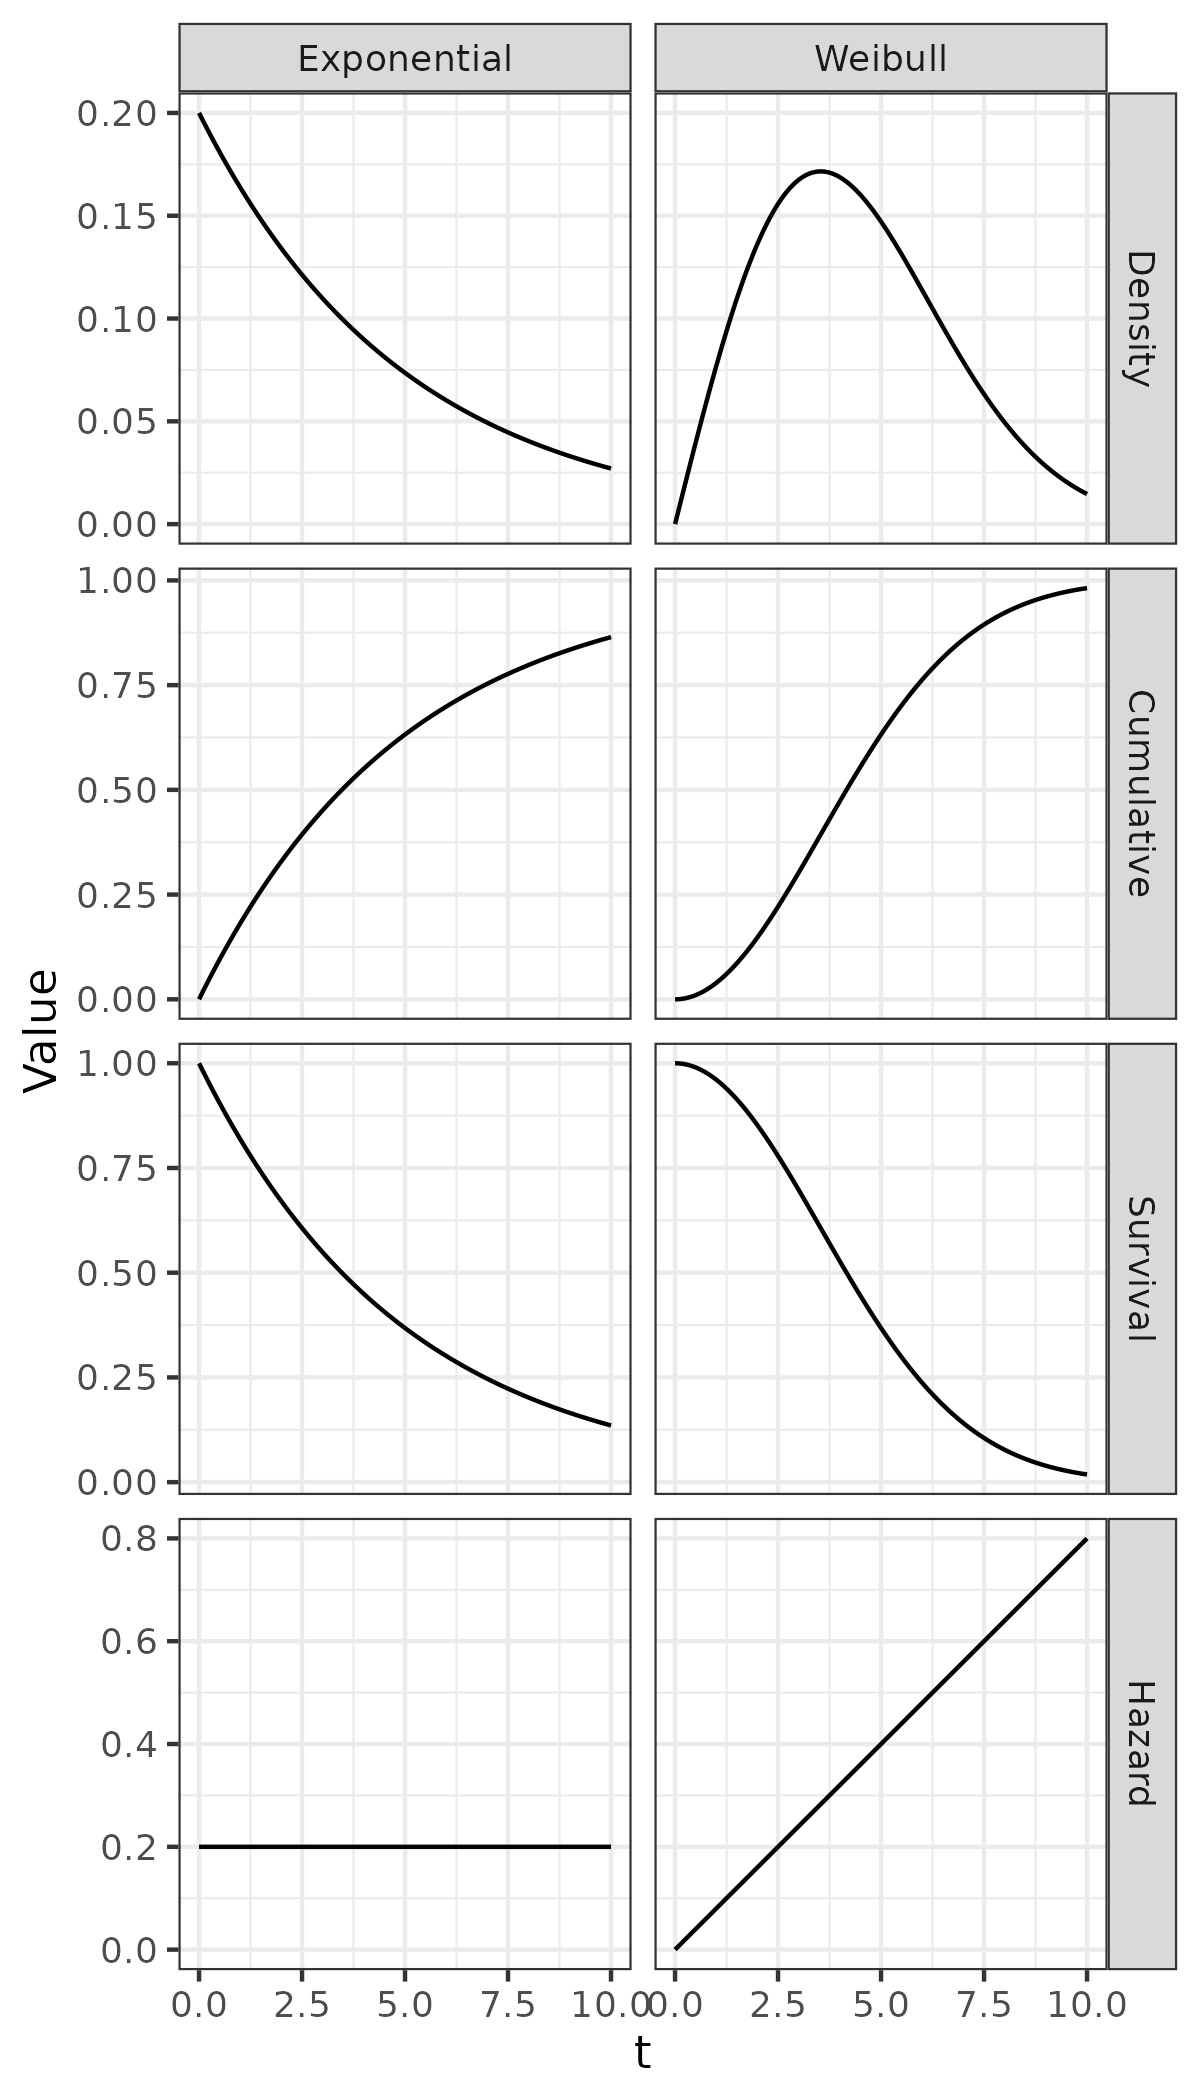
\includegraphics{figures/weiExpFig.png}
\caption{Comparing an Exponential distribution and Weibull distributions
with equivalent rate shape parameters}
\end{figure}

Additionally, see table 1.1 for a comparison of the density, survival,
and hazard functions for the exponential distribution and the Weibull
distribution.



\begin{table}
    \centering
    \begin{tabular}{ccc}
        Function & Exponential & Weibull \\
        f(t) & \(\lambda e^{-\lambda t}\) &
\(\lambda\gamma t^{\gamma-1}e^{-\lambda t^{\gamma}}\) \\
        S(t) & \(e^{-\lambda t}\) & \(e^{-\lambda t^\gamma}\) \\
        h(t) & \(\lambda\) & \(\lambda \gamma ^{\gamma - 1}\) \\
    \end{tabular}
    \caption{Comparison of the Exponential and Weibull distributions
density, survival, and hazards functions.}
    \label{tab:my_label}
\end{table}

The benefits of using a parametric distribution for time-to-event
analysis include its ability to estimate the model using techniques such
as maximum likelihood (Carroll, 2003; Ikbal et al., Mar-2022). This is
important when expanding the Weibull regression to incorporate
predictors into the model.

Examples of time-to-event analysis using Weibull regression are more
readily found in fields such as engineering and economics. Engineering
typically utilizes the Weibull distribution to estimate time-to-failure
for components in some form of design. For example Weibull regression
has been used to study the lifespan of bridges (van Noortwijk \&
Klatter, 2004), electrical equipment (Reddy et al., 2021), and others.
Examples found in economics have examined time spent unemployed
(Dell'Aringa \& Lodovici, 1988), additional multilevel examples of the
same topic are also found in the economics literature (Sohn et al.,
2007).

Examples of psychological literature applying Weibull regression can be
found in examinations of work absenteeism (Fichman, 1989), and
multilevel approaches for the estimation of response times (Kay \&
Kinnersley, 2002).

In summary, hazards estimated from a Weibull model are extremely
flexible. A lot of natural phenomenon may not follow an exponential
distribution's static fixed hazard rate, the Weibull model can
accommodate monotonically increasing or decreasing hazard function.

\section{Semi-Markov Models}
The estimation of the Markov model is facilitated by two assumptions:
state transitions are only influenced by the current state, and these
transitions are time homogeneous. The semi-Markov model relaxes the
second of these assumptions by allowing for transitions to be influenced
by a ``local clock''. The concept of a local clock details how the
transition probability is influenced by the time a state has been
occupied (Boyd \& Lau, 1998). This relaxes the ``memoryless'' property
of the continuous-time Markov model, which adheres to the exponential
distribution to determine transition probabilities at a point of time.
One of the more commonly applied distributions used to estimation
transition intensities for semi-Markov models includes the Weibull
distribution (Asanjarani et al., 2022; Ikbal et al., Mar-2022).

The utility of these semi-Markov models, and the relaxation of the
``memoryless'' property is best underscored by examining their
application to clinical data. For example, when applying a survival
model examining transition from life into death in a population of
cancerous patients, it is important for the model to respect the nature
of cancerous cell growth. A hallmark of cancer is the exponential growth
of tumors thus the longer a life threatening tumor is present the more
likely a transition is to occur. The Weibull distribution is capable of
incorporating these accelerated time-to-event features into the
estimation of hazards, all in a parametric fashion (Van Wijk \&
Simonsson, 2022; Wei, 1992).

Given its increased flexibility, the estimation of semi-Markov models is
inherently more difficult. The goal of the continuous-time Markov model
is to estimate the most probable state at a specific point in time. This
is facilitated by the two assumptions of the Markov model. Relaxing the
``memoryless'' assumption now means the most probable state occupied at
a point in time is dependent upon the local clock, and the current
state. Typically, a continuous-time Markov model is solved via a series
of differential equations. For every state, a differential equation
is estimated examining transitions into and out of this state (Boyd \&
Lau, 1998; Jackson, 2011). This modeling is facilitated largely by the
constant nature of these transition intensities; however, when a
semi-Markov model approach is applied these become more difficulty to
estimate. Solutions for semi-Markov model are typically solved by
parametric estimation by examination of the sojourn times. Specifically,
the logarithm of the sojourn times can be regressed onto a function, and
the likelihood of this function can be maximized to match the
distribution of the observed transition times (Król \& Saint-Pierre,
2015; Wei, 1992).

\section{The Equivalence of Continuous-Time Semi-Markov Models and Survival Analysis}
As may be apparent now, the survival model and the Markov model share
many underpinnings. Both of these techniques seek to identify the time
until a transition is to occur. In order to perform this, ``hazards'' of
an event occurring given the current state of an individual at a
specific point of time are estimated. The most basic form of the
survival model seeks to identify a transition from ``life'' into a
``death'' state. In this formulation of the model, one cannot transition
out of the death state, and thus the death state is known as an
absorbing state (Meira-Machado et al., 2009). Alternatives to the
two-state survival model are known as multistate models. In these
examples, there may be an additional ``diseased'' state which
participants can exist. In these continuous-time multistate survival
models, the formulation is identical to that of the continuous-time
Markov model (Asanjarani et al., 2022); however, one benefit of viewing
the problem as a time-to-event analysis is the ability to utilize
parametric distributions outside of the exponential distribution to
model the hazards, as is employed in the estimation of semi-Markov
models (Król \& Saint-Pierre, 2015).

In order to navigate between the sojourn analysis and the multistate
transition intensity estimation of the Markov model it is important to
describe some foundation parameters in these models. Translating between
the sojourn analyses and the Markov models begins with the elementary
components of a Markov model: the homogeneous Markov chain,
\(\{X_{n}\}_{n \geq 0}\) where \(X\) is a stochastic process generated
from states \(\{1,2,...,S\}\) where the probability of nth jump from
state \(i\) to state \(j\) for \(i \neq j\) is \(p_{ij}\), formally:

\[p_{ij}=P(S_n=j|S_{n-1}=i)\]

The goal of a continuous-time multistate model is to extend these
discrete-state transitions into an instantaneous intensity matrix,
formally:

\[
q_{ij}(t,x_i)=lim_{\Delta t \rightarrow 0} \frac{P(S(t + \Delta t)=s|S(t) = r)}{ \Delta t}
\]

The intensity represents the instantaneous risk of a transition from
state \(i\) into state \(j\) at a specific point in time \(t\). The
intensity matrix forms a matrix that is identical in dimensions to that
of the transition matrix denoted \(Q\). The diagonal elements of the
intensity matrix are estimated as \(q_{ij}=-\Sigma _{i \neq j} q_{ij}\).
Typically, in a time-homogeneous Markov model these intensities are
estimated by fitting an exponential distribution to the observed sojourn
times. The goal of a continuous-time Markov model is to estimate the
probability an individual is in a state at any specific point in time.
In order to model these transitions at a specific point in time the
intensity matrix is used and is estimated as \(\frac{-q_{ij}}{q_{ii}}\).

The semi-Markov model follows an identical framework but assumes the
sojourn times no longer follow an exponential distribution. Examples of
functions that can be used to estimate hazards include the log-normal,
inverse Gaussian, and of course the focus on this dissertation, the
Weibull distribution.

Translating between a model with a constant hazard, and a monotonically
decreasing or increasing hazard requires estimating the hazard function
that best fits the observed transitions \(X\), and the time of these
transitions \(T\). Translating between the hazards of a single
transition and a multistate transition is established with the following
relationship (Asanjarani et al., 2022 ; Król \& Saint-Pierre, 2015):

\[
\lambda_{ij}(t) = \frac{p_{ij}S_{ij}(t)}{S_{i}(t)}f_{ij}(t) = p_{ij}\frac{f_{ij}(t)}{S_{i}(t)}
\]

Here, \(\lambda_{ij}\) represents the instantaneous hazards of a
transition occurring, \(S_{ij}\) is the survival function for a
transition from state i into state j, \(S_{i}\) is the survival
function for all emissions from state i, and finally \(f_{ij}\) is the
density function for transitions from state i into state j. This formula
allows for the translation between the sojourn analysis typically
employed in time-to-event analyses, and continuous-time multistate
models. In fact, one of the main benefits of the simplicity of this
model, is that bearing some restrictions, most distributions that are
appropriate to apply for time-to-event analyses, can now be used for
these continuous-time multistate analyses. The updated hazards for a
Weibull multi-state time-to-event analysis now take the following form:

\[
\lambda_{ij}(t)=p_{ij}\frac{\eta_{ij}}{\mu_{ij}}(\frac{t}{\mu_{ij}})^{\eta_{ij}-1}=\frac{\eta_{ij}}{p_{ij}^{-1/\eta_{ij}}\mu_{ij}}(\frac{t}{p_{ij}^{-1/\eta_{ij}}\mu_{ij}})^{\eta_{ij}-1}
\]

Notably, the scale parameter of the Weibull distribution assumes the
following form \(p_{ij}^{\frac{-1}{\eta_{ij}}}\mu_{ij}\) while the shape
parameter is the same as prior (Asanjarani et al., 2022). This allows
for a Weibull time-to-event analysis to be translated into a
continuous-time semi-Markov model. Additionally, as the models are
Weibull regression, the same inferences can be made on these hazards as
is performed in survival analysis, as well as the same extension to
include frailty terms.

\section{Alternatives to Multilevel Markov and semi-Markov Models}
Alternatives to the multilevel Markov model must be considered given the
data present to the researcher and the questions that are sought to be
answered. The multilevel semi-Markov model can be used when the analyses
seek to generalize across a heterogeneous population and the data are
composed of manifest discrete-states. Alternative methodology may be
best applied when alternative scenarios exist. For instance, one of the
more commonly applied methodological tool is the hidden Markov model
(Visser et al., 2002).

The hidden Markov model is appropriate when multiple streams are data
acquired for every participant at each timepoint, and the manifest
states are not present in the data. These methods have similar
multilevel extensions which allow them to incorporate transition
differences across individuals (de Haan-Rietdijk et al., 2017), as well
as semi-Markov extensions (Yu, 2010).

One final methodological consideration is the source of potential
heterogeneity observed in participants. If the source of the
heterogeneity is potentially derived from sampling across populations
with different dynamics, then a mixture Markov model may be more
appropriate (Maruotti \& Rocci, 2012). For the mixture Markov model, the
assumption is that participants are sampled from latent groups, and
these groups have homogeneous transition patterns within themselves.

Each of these methods have their own benefits and drawbacks. The biggest
drawbacks for the multilevel Markov and semi-Markov model is model
identification, there are arguments that these models cannot be
estimated in a frequentists framework if the complexity of the random
effects is too large generally necessitating Bayesian approaches
(Altman, 2007; Seltman, 2002). Of course, if the researchers are
concerned about measurement error, and have the data to estimate a
hidden Markov model, then these hidden Markov models can reduce some
concerns of measurement error. The drawback to this is of course the
proper identification of the number of clusters, and identification of
the starting state for every participant. The same problem exists for
the mixture Markov models, but instead of the number of states the
concern is the correct identification of the number of mixture groups
that are being sampled within.

\section{Review}
The application of Markov, and semi-Markov models is equivalent to multi-state
time-to-event analyses under the correct parameterization. Under such parameterizations, benefits
from both models can be incorporated.
Hazard functions, such as the Weibull, and frailty modeling
can be drawn from the survival analysis literature. This allows for multilevel Markov and semi-Markov models to be estimated. Additionally, these
models can be estimated in fully parametric techniques allowing for a
flexible approach to be applied for model estimation (e.g.~Maximum
Likelihood and Bayesian). The Markov assumption, and the ease of
interpretation can be drawn from the Markov modeling framework for
explanation and description of sample and population characteristics.
This dissertation seeks to describe, and emphasize the benefits of this
merged analytic stream using both a simulation study, as well as an
empirical study. The simulation study will examine parameter recovery
capabilities of time-to-event models under various formulations, the
empirical study will showcase how inferences can be made using these
models to examine population dynamics.


\chapter{Simulation Study}\label{chap:SimulationStudy}
\section{Introduction}
Simulated data are the testing ground for methodological studies as it
allows researchers to examine the capability for a naive model to
identify the true population characteristics in a controlled system.
Specifically, because data are created using a mechanism where all
parameters are known, when a naive model is estimated under varying
simulation factors, differences between the estimated and the true
parameters can be measured. This simulation study seeks to follow this
framework to examine several specific questions about the analysis of
manifest state time series. Specifically these will examine the
performance of time-to-event analyses with and without the memoryless
property constraint, as well as examining the influence that
intra-cluster correlation contributes to these analyses. This requires
simulating data under various data generation mechanisms and to estimate
a series of time-to-event models using both multilevel and without
multilevel components. The specific question this simulation study seeks
to answer include:

\begin{itemize}
\tightlist
\item
  How well does an exponential time-to-event model estimate a criterion
  variables true magnitude when data are generated from a distribution
  with constant and nonconstant hazards
\item
  How well does a Weibull time-to-event model estimate the true
  magnitude of a criterion variable when data are generated from a
  distribution with constant and nonconstant hazards
\end{itemize}

\begin{itemize}
\item
  How well can a Weibull model pick up on the true shape parameter being
  used to generate data
\item
  How much misestimation of the true shape a parameter influence the
  fixed effect parameter estimation
\item
  How well do the confidence intervals from each of these models recover
  the true population parameter
\end{itemize}

Each of these questions also examine the influence random variance has
when answering these questions. That is, when data are generated with
non-negligible random variance, how well do these models perform when
the model includes or excludes a random effect term. In the survival
framework, these means to include frailty terms when simulating the data
with levels of variance in the term. The specific steps performed to
estimate these effects are further explained upon below.

\section{Methods}
In order to answer these questions several discrete steps had to be
performed. First, data were generated with known parameters varying
several common characteristics of an intensive longitudinal design.
Second, four separate models were estimated, two continuous-time Markov
models, one including a random effect, and two semi-Markov models, using
Weibull regression, also one including a random effect. Third, the
inferential capabilities of the various model estimation methods were
compared by identifying estimated parameters with the ground truth, this
process was performed examining both the root mean squared error
(\(RMSE = \sqrt{\frac{\Sigma_{i=1}^N(\theta_{true}-\theta_{estimate})}{N}}\))
as well as a significance framework. The significance framework required
identifying if a parameter had a 0 effect when in reality the true
effect was or was not 0, as well as if the true parameter was included
within the credible interval estimated within the model. The third step
was carried out using both an ANOVA framework, as well as a generalized
linear regression framework. All analyses were carried out using the R
language (R. C. Team, 2020), all models were estimated using STAN (S. D.
Team, 2023), all code is available online
\href{https://github.com/adrose/dissertationSim}{here}.

\subsection{Simulation Factors}
Data were were created by sampling sojourn times from a Weibull
distribution when varying seven separate factors, these factors
included: the total sample size, the minimum number of observations
taken within a simulated individual's time series, the transition
patterns between states, the range of the Weibull scale values selected
to generate sojourn times, the Weibull shape values, the main effect of
the criterion variable, and finally the magnitude of the random
variance. The simulation conditions across each level are found in table 2.1.


\begin{table}
    \centering
    \begin{tabular}{cc}
         Factor & Levels\\
         Sample Size & 20; 100\\
         Observation Length & 20; 40\\
         Population Transition Matrix & Stable; Random\\
         Weibull Scale Range & .5-5; 5-10\\
         Weibull Shape Parameter & 1; 3\\
         Criterion Variable Magnitude & 0; .8\\
         Random Effect Variance & 0; 1\\
    \end{tabular}
    \caption{Factors to be manipulated in simulation study}
    \label{tab:my_label}
\end{table}

A total of 1,000 samples were drawn within every factor yielding a total
of \(2^7 \times 1,000 = 128,000\) total samples. Within every sample, a
total of four models were estimated, two Markov (i.e.~exponential)
models, two semi-Markov (i.e.~Weibull) models, and two models including
random intercepts. In total \(512,000\) total unique models are
estimated which are to be included in all subsequent analyses.

Each of these parameters are taken to exaggerate the Markov modeling
parameters that exist and are commonly observed in the psychological
literature found using these models. For example, sample sizes in some
of the earlier literature utilizing Markov models applied a limited
sample size, for example Miller had a sample size of 10 participants
(Miller, 1952). More recent studies have seen a growth in participant
sizes such as the work by Vogelsmeier and peers which capitalized on EMA
to examine depression symptoms in more than 160 participants overtime
(Vogelsmeier et al., 2021). The sample size reflects the number of
unique individuals that will provide a distinct time series. This is
important because as the random variance increases, the state transition
patterns observed within individuals will become more distinct within
every unique individual.

The second factor manipulated is the length of a time series within
every individual. This varies the amount of information that a specific
individual provides to the model. In order to create an observation
length for every unique individual, every participant has an observation
length sampled from a uniform distribution. The minimum are detailed in
table 2, and the maximum values are twice the minimum. For example, if
the minimum observation length was 20, then every participants
observation length was randomly sampled from a uniform distribution with
a minimum of 20 and a maximum of 40 observations. The minimum value was
selected based on the definition of intensive longitudinal data in the
behavioral sciences suggesting that more than 20 observations within
individual's justifies the application of time series analytic
methodology (Asparouhov et al., 2018).

The third factor was the population transition matrix which describes
the probability that a state is selected given the current state of an
individual. Two population transition matrices were used, a stable
matrix where emission probabilities were strongest for the current
state, and a random matrix where emission probabilities were equivalent
across all possible states. Example two-state transition matrices are
provided below:

\[
P_{stable} = \begin{pmatrix} .8 & .2 \\ .2  & .8 \end{pmatrix}
;
P_{random} = \begin{pmatrix} .5 & .5 \\ .5  & .5 \end{pmatrix}
\]

This alters the amount of information that is present for each
transition pattern. Because every unique transition will have it's own
specific Weibull scale parameter, the more observations of a specific
transition provide more information to the model to estimate what the
true transition rates are for every distinct transition pattern. Thus,
it is hypothesized that Weibull models will recover parameters better
when a random transition matrix is used.

Two parameters must be sampled when in order to sample sojourn times from
a Weibull distribution , a scale and a shape parameter. The Weibull
distributions true scale range was used to sample the population fixed
effect for every transition. A uniform distributions had either a
minimum value of .5 or 5, and a maximum value of 5, or 10. When the
Weibull distribution has a lower scale range, the time-to-event
distributions would be less scaled to the right, and sojourn times would
be closer to 0. The longer distribution allows for greater information
when hazards which may deviate from the exponential distribution. The
hypothesis is that both the shape and criterion parameter will be more
difficult to recover with lower scale parameters

The Weibull shape parameter was used to determine if hazards were
constant, or monotonically increasing. Specifically, when the Weibull
shape parameter is ``1'' the memoryless property of the Markov model is
satisfied. Thus the hazards of an event (i.e.~a transition) occurring
are constant. When the shape parameter is 3, the hazards of an event
increase the longer a state is maintained, thus the memoryless property
is not satisfied. This means that the time spent within a state
determines influences that hazards such that the longer a state is
maintained the more likely a transition is to occur. It is hypothesized
that estimation error will be the highest when shape parameters are
mismatched, that is, when an exponential model is fitted to a Weibull
model. However, the Weibull model is capable of recovering an
exponential distribution, which may potentially reduced this concern
when a semi-Markov approach is taken.

The magnitude of the criterion variable was chosen between a null effect
and a relatively large magnitude. This criterion variable acts
uniformly across all scale parameters included in the model. A time
invariant predictor is sampled from a normal distribution
(\(N(\mu=0,\sigma=1)\)) for every participant contributing a unique time
series. This predictor then creates a main effect acting on the scale
parameters of the distribution with either a 0 effect or an effect of
relatively large magnitude 0.8.

Finally, the last variable manipulated was the magnitude of the random
variance. Random variance in these models influences the hazards across
all transitions. In the survival vernacular this is the frailty term, in
a Markov vernacular this influences an individual's propensity to stay
or move between states. This will be exhibited in the sojourn times,
participants with a random effect greater than 0 will have longer
sojourn times. Two variances were selected either none, or large. The
motivation here was to see how well subject specific patterns influence
the inferential capabilities of these models. The hypothesis states that
a multilevel modeling framework will protect against larger variance,
and a fixed effect modeling approach will see increased error when
random variance increases.

\subsection{Model Fitting}\label{subsec:reference_prior}
After having simulated the data, the next step is to measure how well a
naive model can recreate the population parameters using four different
methods. The methods include:

\begin{itemize}
\item
  An exponential time-to-event model (i.e.~continuous-time Markov model)
\item
  A multilevel exponential time-to-event model (i.e.~multilevel
  continuous-time Markov model)
\item
  A Weibull time-to-event model (i.e.~continuous-time semi-Markov model)
\item
  A multilevel Weibull time-to-event model (i.e.~multilevel
  continuous-time semi-Markov model)
\end{itemize}

Consistent across all models were the fixed effect parameters to be
estimated. In order to parameterize a continuous-time discrete-state
Markov model a shape parameter has to be estimated for every inter-state
transition. For a three-state transition matrix this requires the
estimation of an intercept term and 5 additional fixed effects. On top
of this, a criterion variable acting across all main effects was to be
estimated. For the continuous-time Markov model a time-to-event analysis
was used assuming the sojourn times followed an exponential
distribution. For the multilevel continuous-time Markov model,
participant specific random intercept term was included and sojourn
times were again assumed to follow an exponential distribution. For the
continuous-time semi-Markov model, a time-to-event analysis was
estimated by modeling the sojourn times with a Weibull distribution. The
multilevel continuous-time semi-Markov model included a participant
specific intercept.

All models were estimated using a Bayesian framework. Specifics to the
fitting process include a warm-up period using a total of 2,000
iterations, a sampling period which included 5,000 iterations, thinning
included every 3 sample generated, and a total of 3 chains were sampled.
Diffuse and uninformed priors were included. All sampling was performed
using the STAN language using the No U-turn Sampler (NUTS) algorithm
(Homan \& Gelman, 2014; S. D. Team, 2023).

\subsection{Assessment of Model Performance} \label{sec:Inference_methods}
In order to answer the specific questions the simulation study seeks to
answer several models had to be estimated. The first model, the most
general identifies parameter error across all models when comparing the
estimated criterion variables magnitude with the true parameter. In
order to identify any error attributed to specific simulation factors
the parameter estimation error was modeled as the root of the squared
error (\(\sqrt{(\theta_{estimate}-\theta_{true})^2}\); RSE) between the
true and the estimated value. The RSE was regressed onto all of the
simulation factors as well as an additional factor indicating which type
of model is being estimated. The models included either a semi-Markov or
a Markov model with or without a multilevel component. Up to all
four-way interactions were included in this ANOVA model. In order to
identify which simulation factors contributed to the estimation error.
This was performed by measuring the \(\eta^2\) of each predictor in the
model. In order to ease interpretation, all \(\eta^2\) values less than
0.01 were excluded from additional examinations. These results will
inform the reader for how much error exists across all models, but
specifically, if the different model estimation techniques reduce error
when comparing across the four modeling approaches.

Next, error was assessed for the Weibull models ability to estimate the
true population shape parameter. An identical procedure was performed as
in the previous analyses, but now the model was constrained to only
include the semi-Markov models. This analysis examines the ability for a
Weibull regression to identify the true shape parameter under the
various simulation factors included in this study.

The third set of analyses examines the coverage of the true main effect
by the 95\% Bayesian credible interval (BCI). The BCI acts as an
alternative to standard error and p-value based approaches for
significance although the interpretation different. The BCI allows
researchers to state the probability that the true effect lies between
the BCI with a specific degree of confidence. The outcome for these
models now examines if the 95\% BCI includes the true population
parameter. For models where the true magnitude of 0, this would require
for the lower BCI interval to be less than 0 and for the upper interval
to be greater than 0. For the models with a large criterion magnitude,
coverage was identified when the model included the parameter but
excluded 0 in the BCI. The coverage was measured using a binary approach
where the parameter was either included or excluded in the 95\% BCI,
this follows recommended practices for Bayesian analyses (Kruschke \&
Liddell, 2018). This binary outcome was then regressed onto all
simulation parameters as well as the model estimation technique used,
similar to the previous ANOVA models.

\section{Results}\label{results}
\subsection{Model Estimation}
All models were successfully estimated although not all models converged
at an acceptable level. Convergence in a Bayesian framework can be
assessed by the scale reduction statistic, which is also known as the
\(\hat{R}\) value. This measures the within- and between-chain parameter
sampling variability, when chains have mixed and convergence is achieved
than the difference between chains will lead to an \(\hat{R}\) value
close to 1. The larger values suggest models did not converge (Gelman \&
Rubin, 1992). A total of 551 models had \(\hat{R}\) values greater than
1.5, of these 517 were from the multilevel Weibull models, and the
remaining 34 were from the multilevel exponential models. All of these
models were excluded form any subsequent analyses, however, it is worth
stating that these convergence issues represent a minority of the total
estimated models (\(0.001\%\)).

\subsection{Criterion Parameter Estimation Error}
The first ANOVA examined the difference between the estimated and true
criterion parameter. The most influential predictors from the ANOVA
model were assessed using the \(\eta^2\) effect size, all values greater
than 0.01 were examined as well as the main effects from the model (see
table 3). The only main effects which had \(\eta^2\) greater than 0.01
were the magnitude of the random variance (\(\eta^2=0.29\)), the sample
size (\(\eta^2=0.15\)), and the model used to estimate the effect
(\(\eta^2=.05\); see figure 2.1).


\begin{table}
    \centering
    \begin{tabular}{cc}
        Parameter & \(\eta^2\) \\
        Magnitude of Random Variance & .29 \\
        Sample Size & .15\\
        Model Strategy & .05 \\
        Sample Size: Magnitude of Random Variance & .10 \\
         Model Strategy: Magnitude of Random Variance & .03 \\
    \end{tabular}
    \caption{Predictors with larger than 0.01 effect sizes from ANOVA
examining criterion variable estimation error}
    \label{tab:my_label}
\end{table}

There were only two separate two-way interactions which had an effect
size larger than 0.01. These include the interaction between the sample
size and the magnitude of the random variance (\(\eta^2 = 0.10\); see
figure 2.2), and the interaction between the modeling strategy and the
magnitude of the random variance (\(\eta^2=0.03\); see figure 2.3). The
interaction between sample size and the magnitude of random variance is
driven by an increase in parameter estimation error when the sample size
is small, and the random variance is large, compared to much lower error
when random variance is not present. The second interaction is driven by
the increase of error specific to the Markov model when random variance
is large, while the remaining techniques error is much closer. Error
across all modeling techniques is consistent when random variance is not
present. No three-way interactions had an effect size larger than 0.01.

\begin{figure}
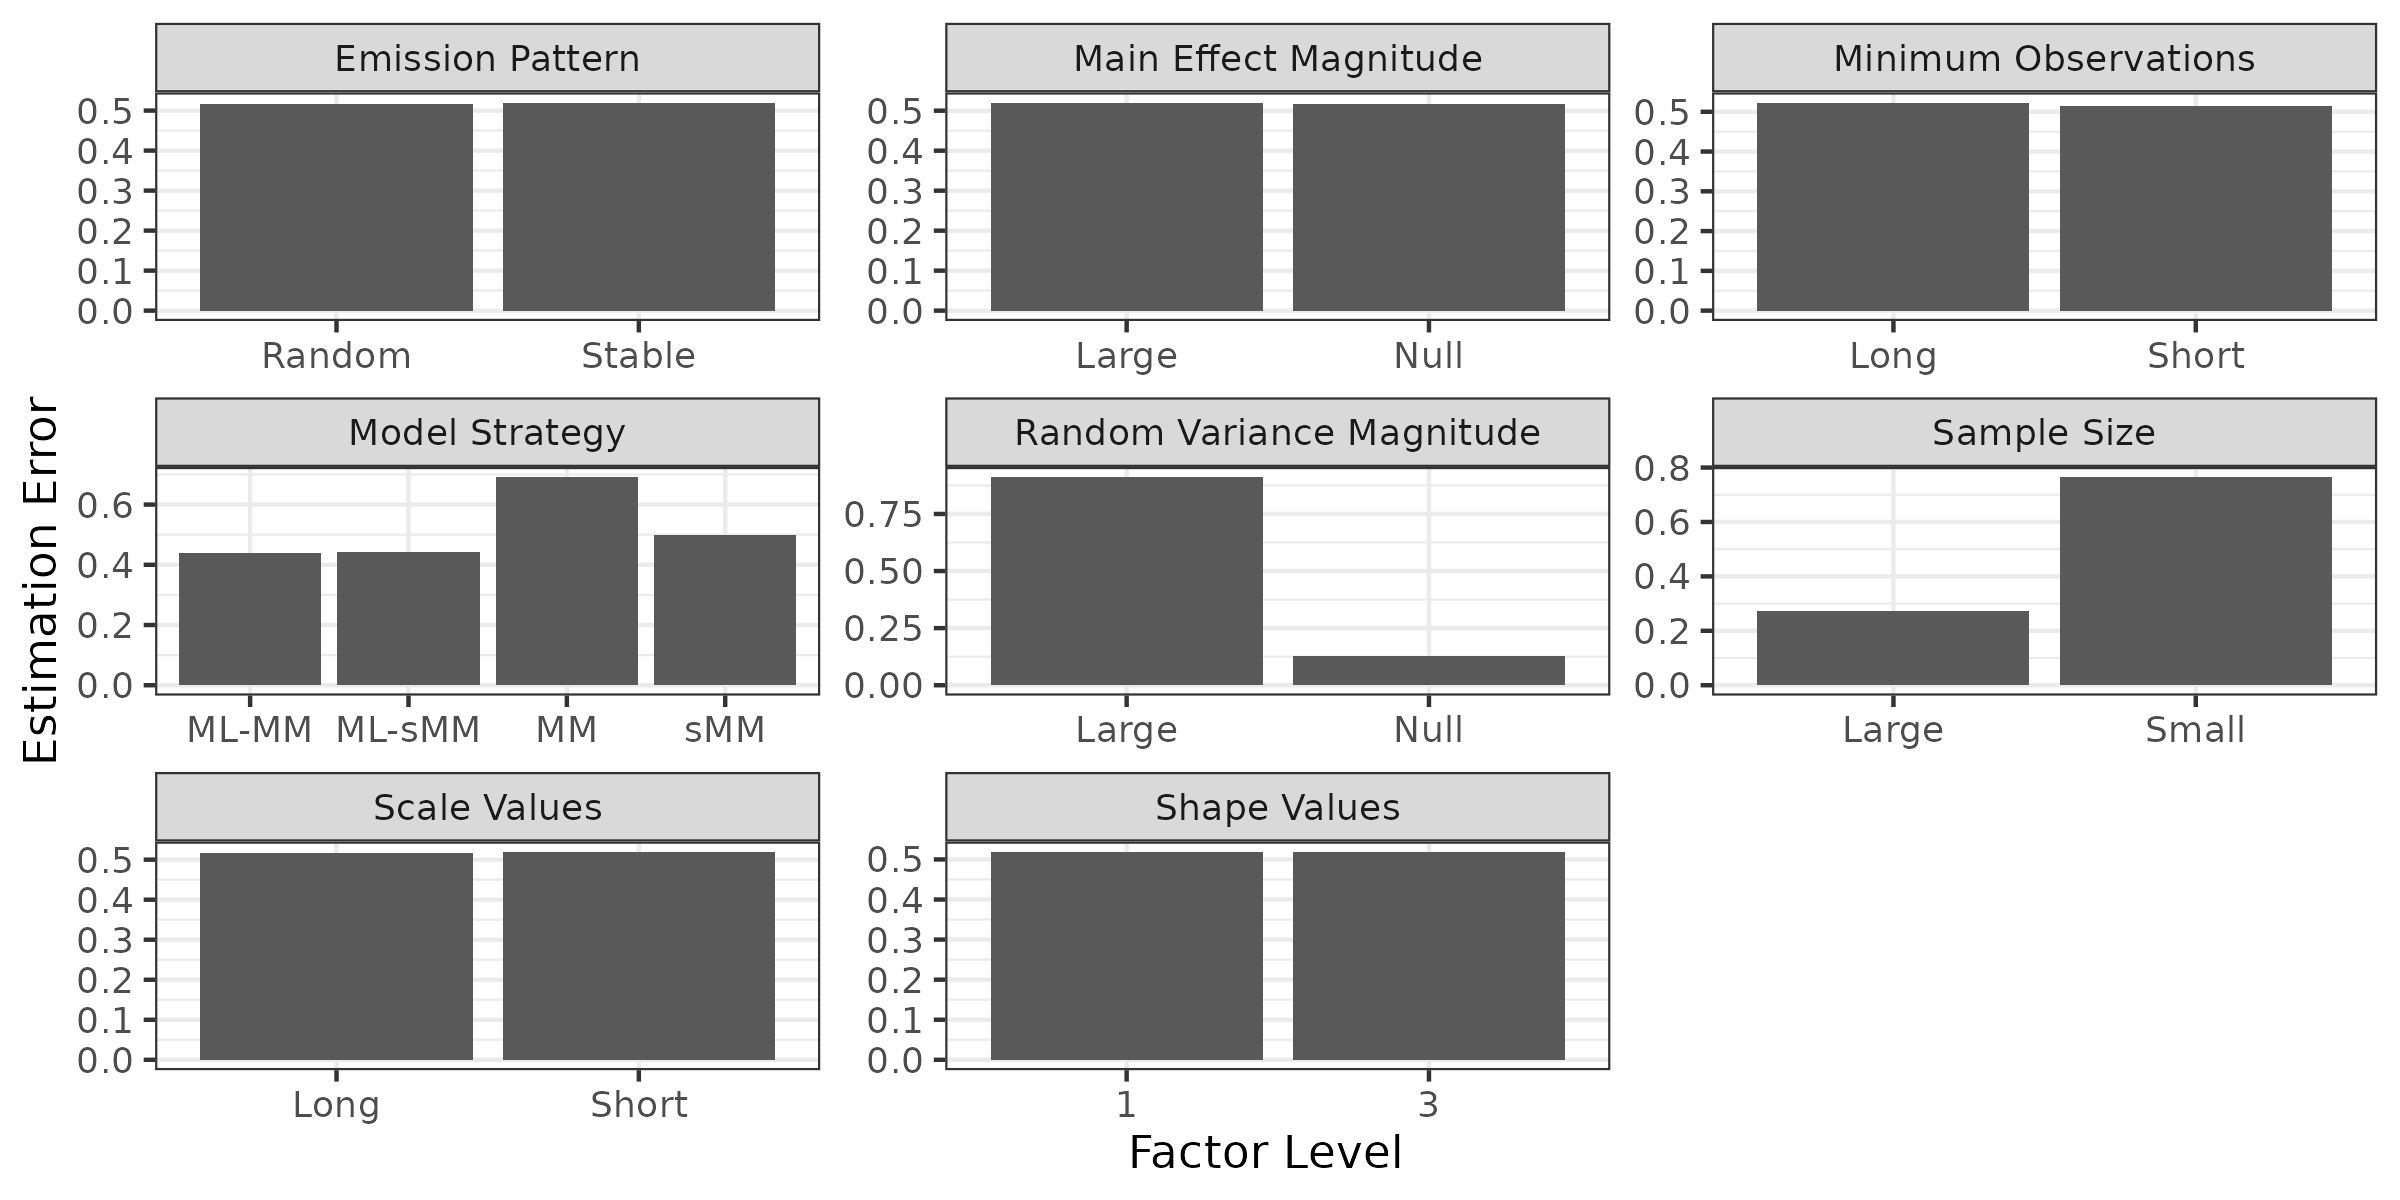
\includegraphics[width=15cm]{figures/anova1MainEffect.png}
\caption{The main effects from an ANOVA examining differences between
the true and estimated effect.}
\end{figure}

\begin{figure}
\centering
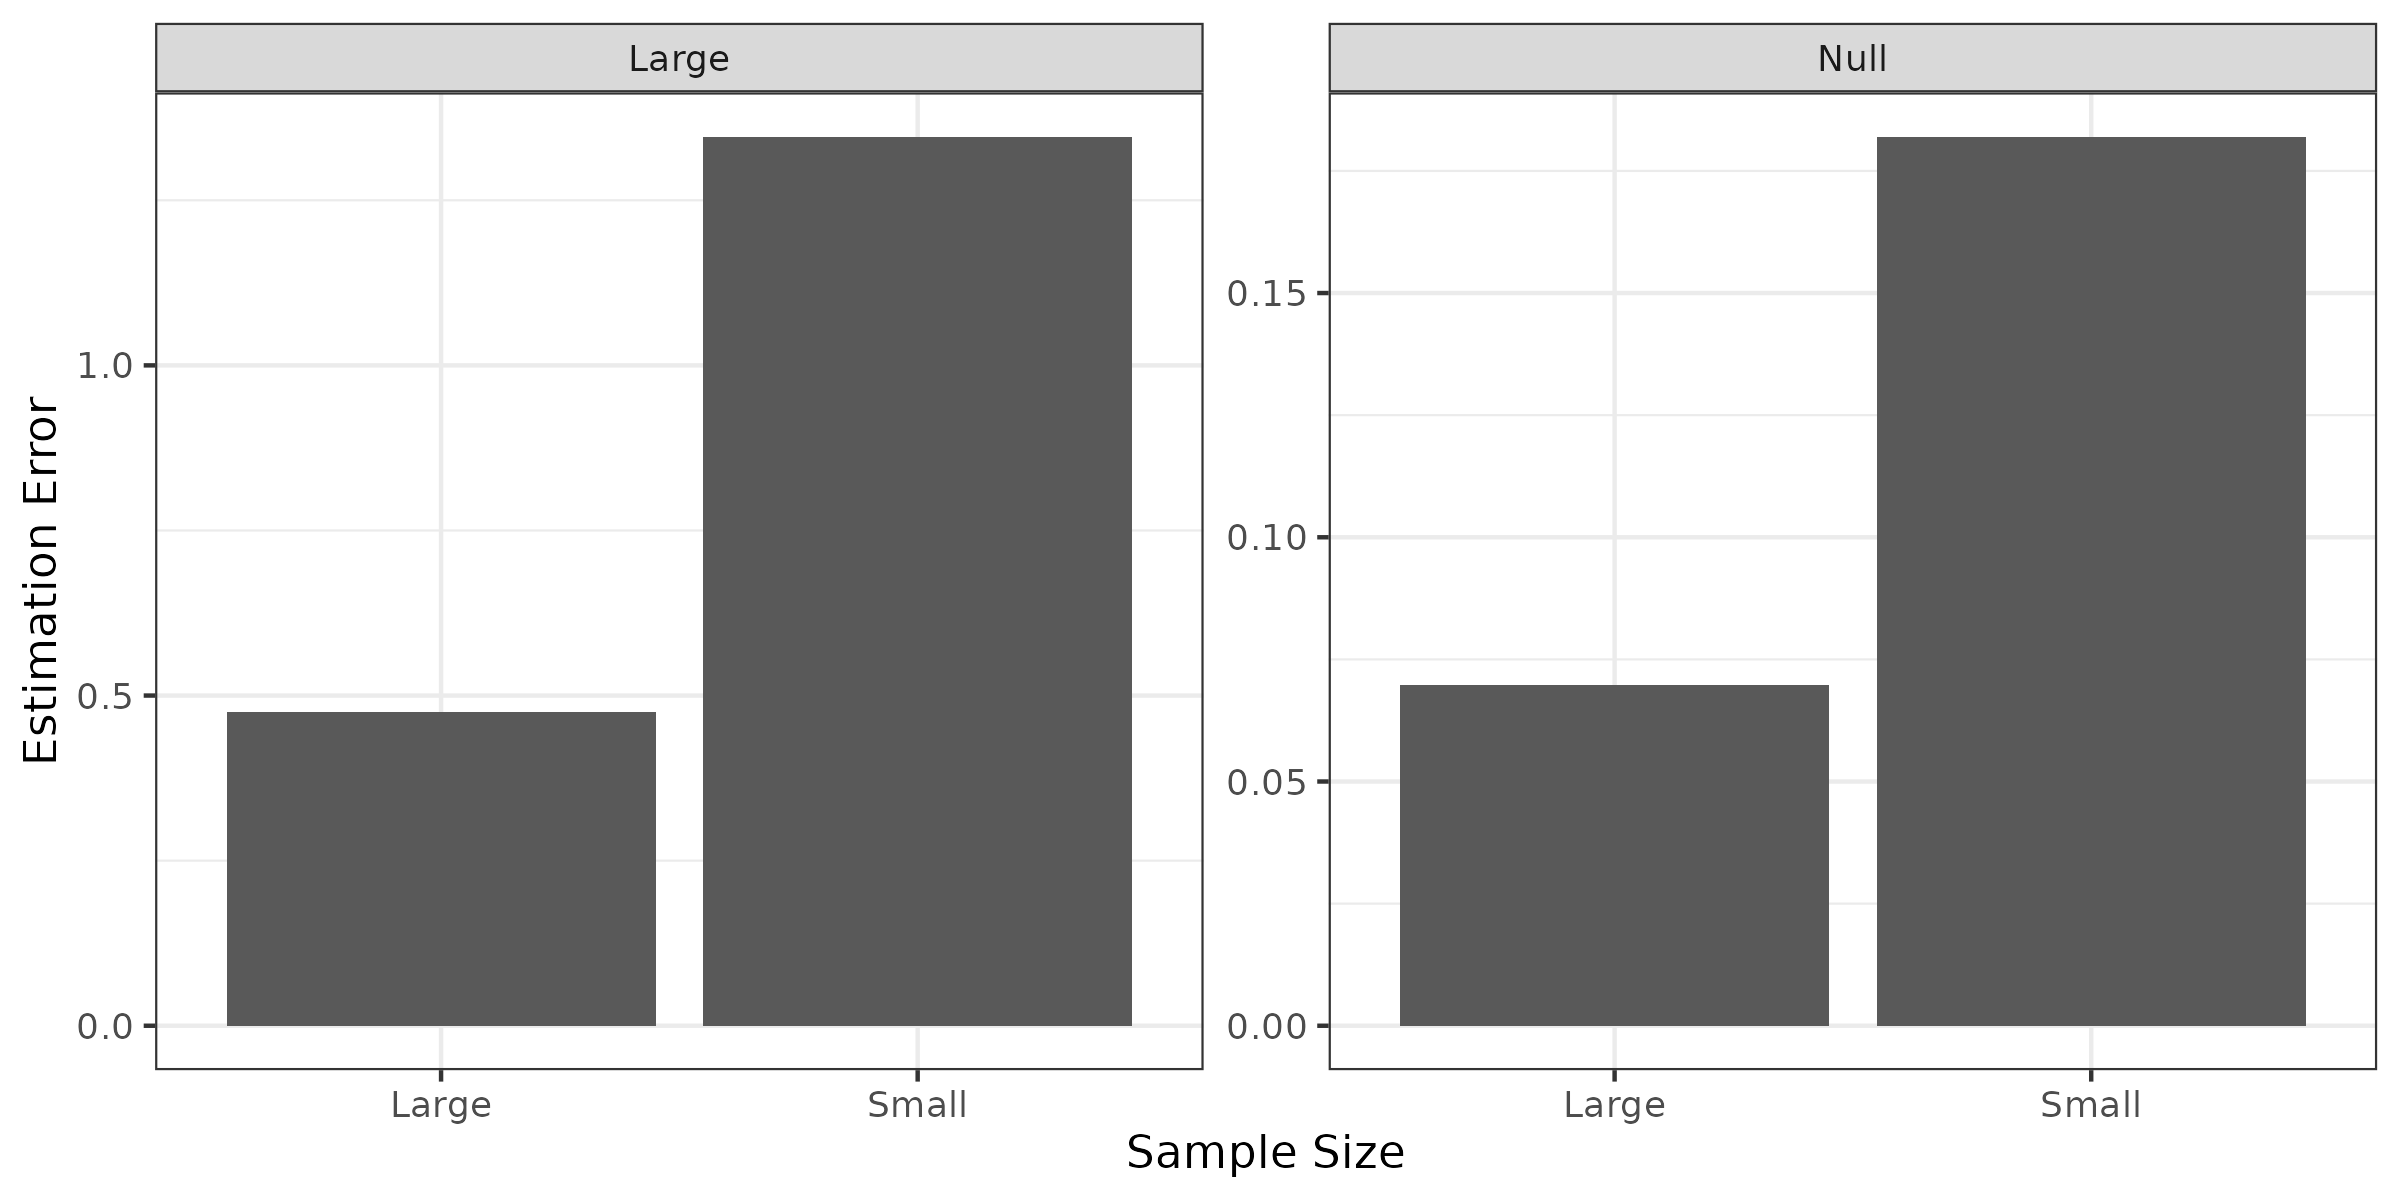
\includegraphics[width=15cm]{figures/anova1TwoWay2.png}
\caption{Two-way interaction between magnitude of random variance and
the sample size}
\end{figure}

\begin{figure}
\centering
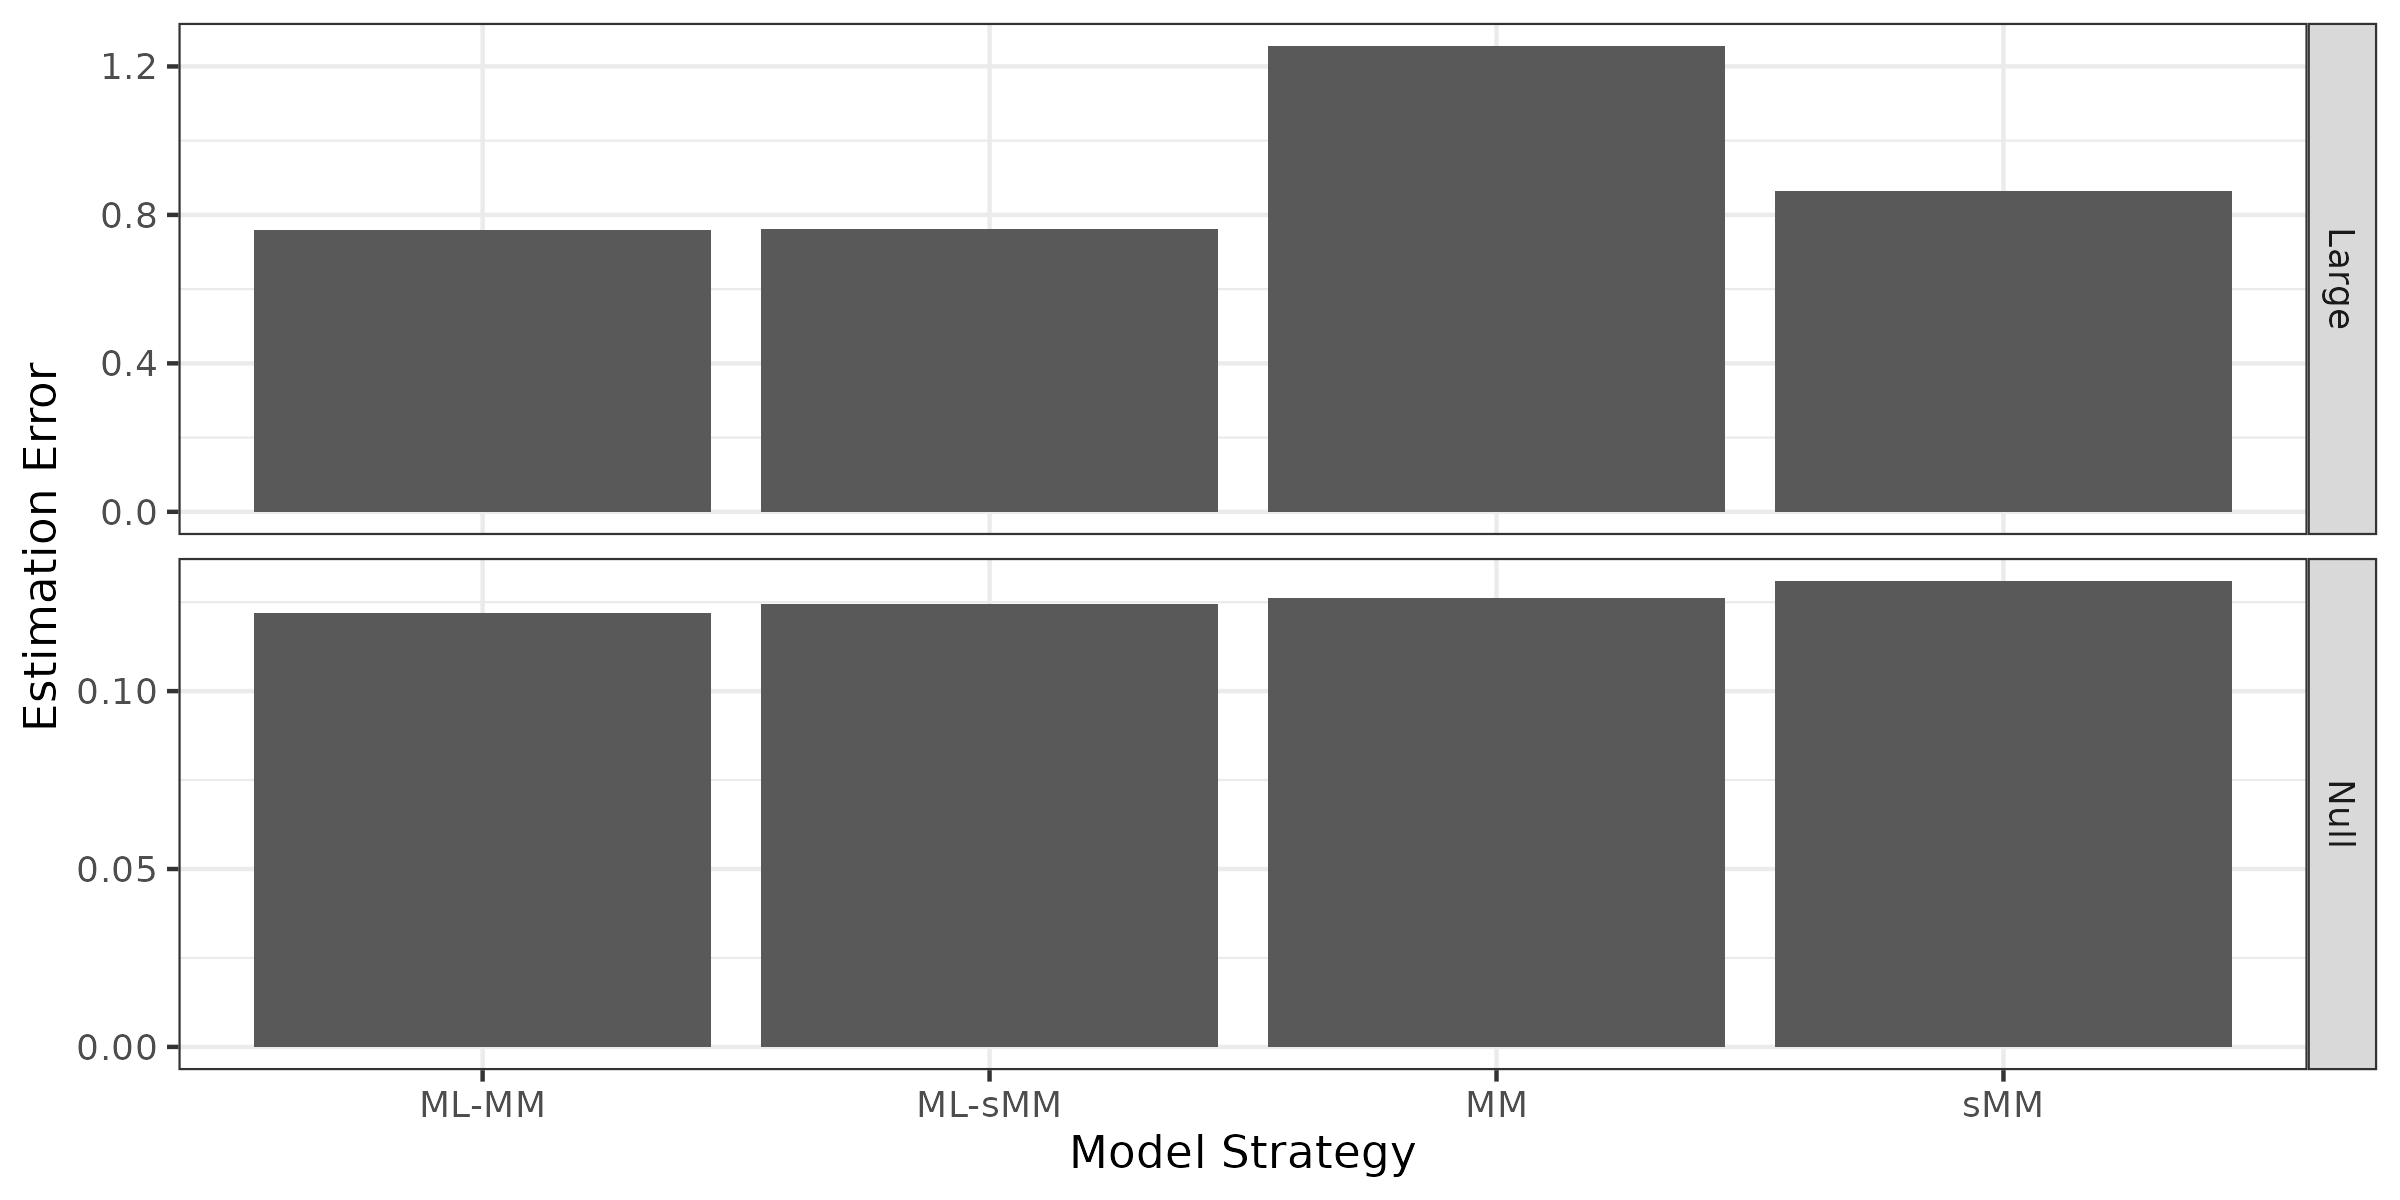
\includegraphics[width=13cm]{figures/anova1TwoWay1.png}
\caption{The two-way interaction between modeling strategy and the
magnitude of the random variance.}
\end{figure}

\newpage
\newpage


\subsection{Shape Estimation Error}

The second analysis examined how well the semi-Markov models can recover
the true shape parameter. The most influential predictors from the ANOVA
were assessed again using the \(\eta^2\) effect size, all main effects
(see figure 5) from the ANOVA and any interaction term with an
\(\eta^2\) greater than 0.01 are further explored. The most influential
main effects include the population shape parameter (\(\eta^2\)=.84),
the model strategy (\(\eta^2\)=0.07), and the magnitude of the random
variance (\(\eta^2\)=0.02; see table 2.3).


\begin{table}
    \centering
    \begin{tabular}{cc}
        Parameter & \(\eta^2\)\\
        Shape Parameter & .84 \\
        Model Strategy & .07 \\
        Magnitude of Random Variance & .02 \\
        Shape Parameter: Model Strategy & .04 \\
        Magnitude of Random Variance: Model Strategy & .03 \\
    \end{tabular}
    \caption{Predictors with larger than 0.01 effect sizes from ANOVA
examining shape estimation error}
    \label{tab:my_label}
\end{table}

The two-way interactions with an \(\eta^2\) greater than 0.01 include
the interaction between the true shape parameter and the model strategy
(\(\eta^2\) = 0.04; see figure 2.5), as well as the interaction between
the magnitude of the random variance and the modeling strategy
(\(\eta^2\) = 0.03; see figure 2.6).The direction of both of these
interactions indicated the multilevel semi-Markov model had lower error
than the fixed effect framework.

\newpage


\begin{figure}
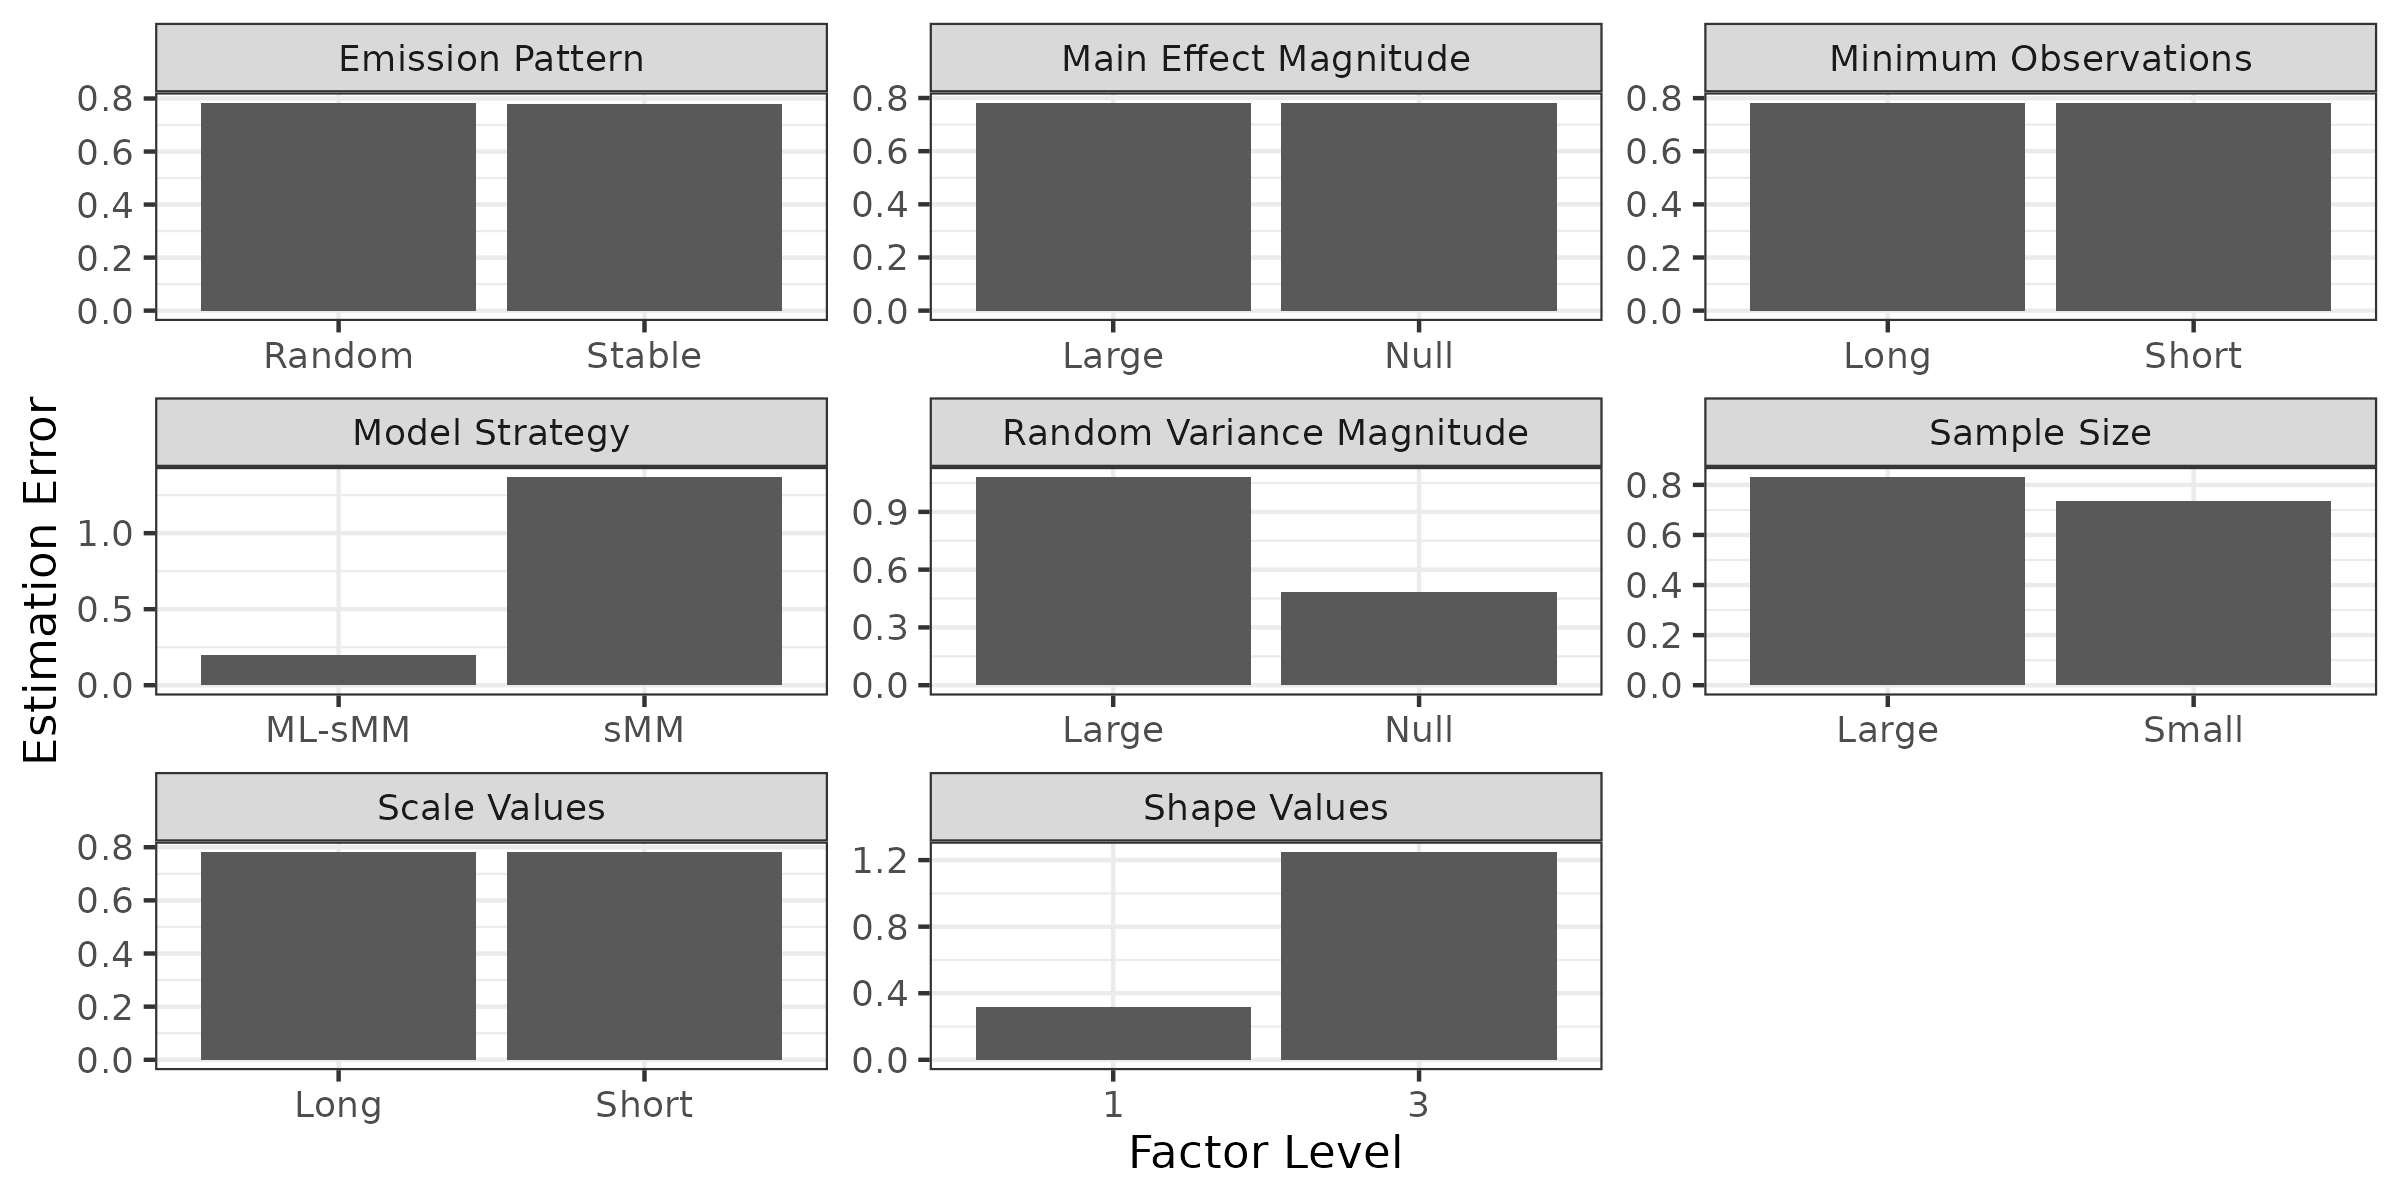
\includegraphics[width=15cm]{figures/anova2MainEffect.png}
\caption{The main effects from an ANOVA examining differences between
the true and estimated shape parameters.}
\end{figure}

\begin{figure}
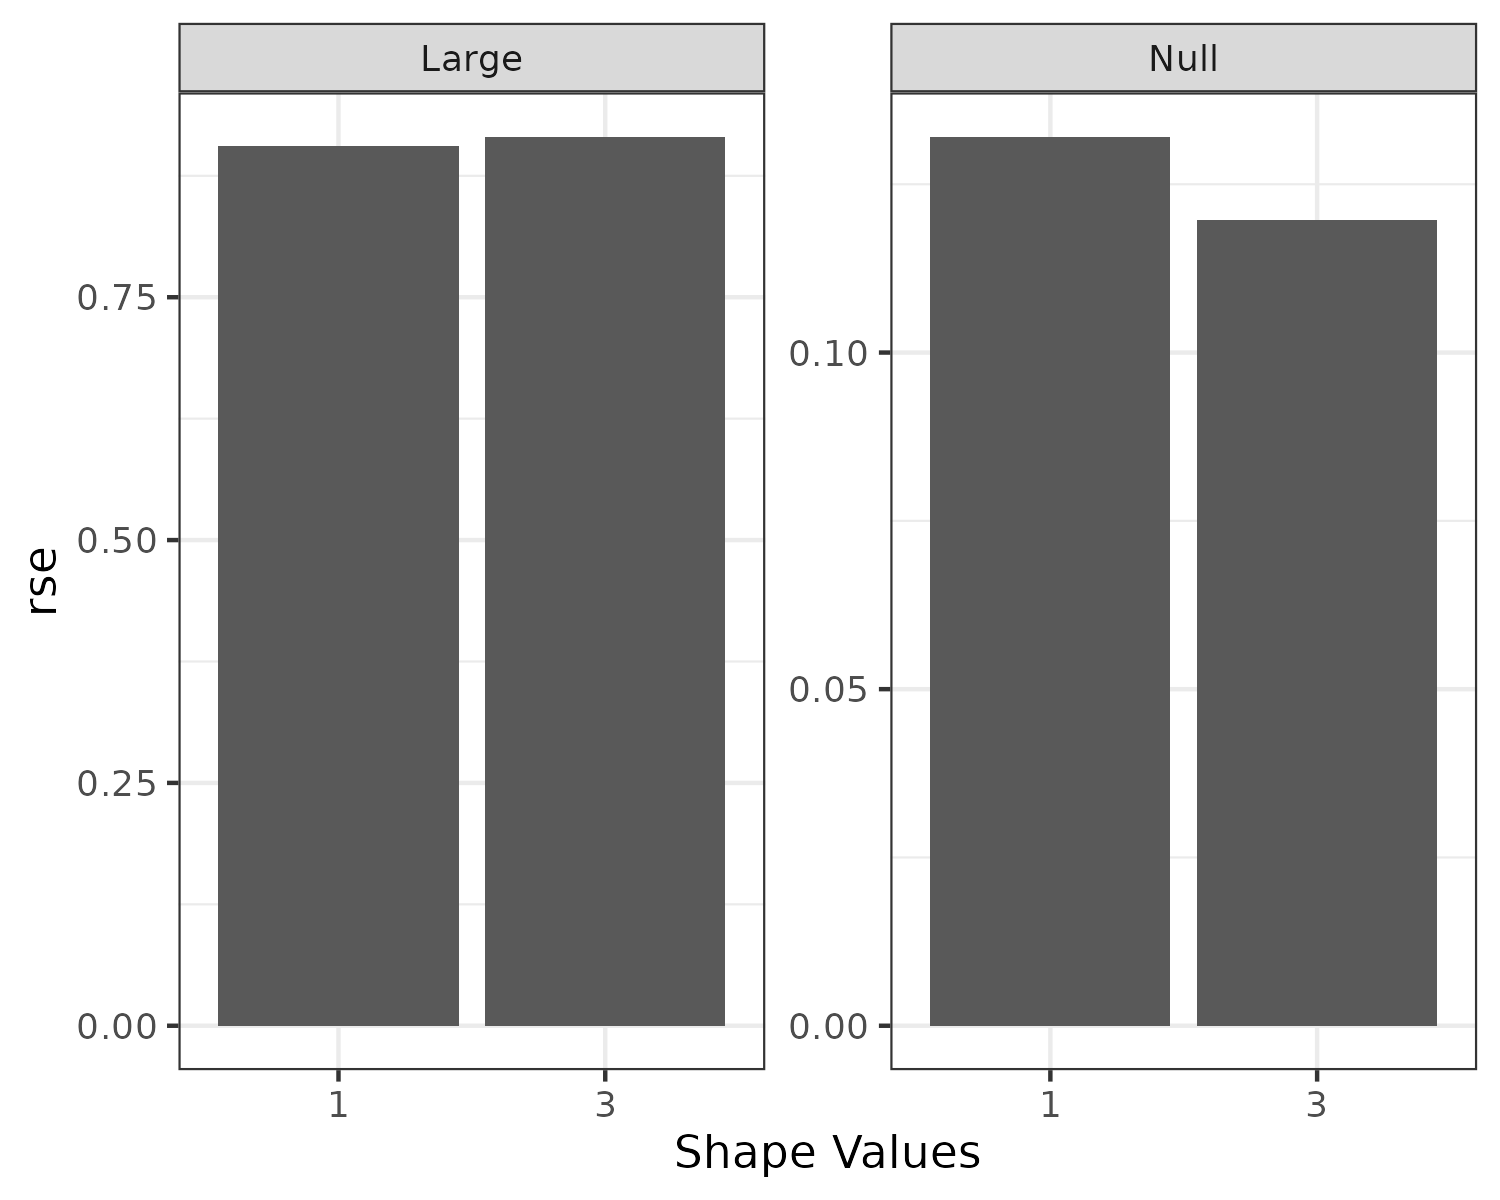
\includegraphics[width=12cm]{figures/anova2TwoWay2.png}
\caption{Two-way interaction from an ANOVA examining differences between
the true and estimate shape parameters}
\end{figure}

\begin{figure}
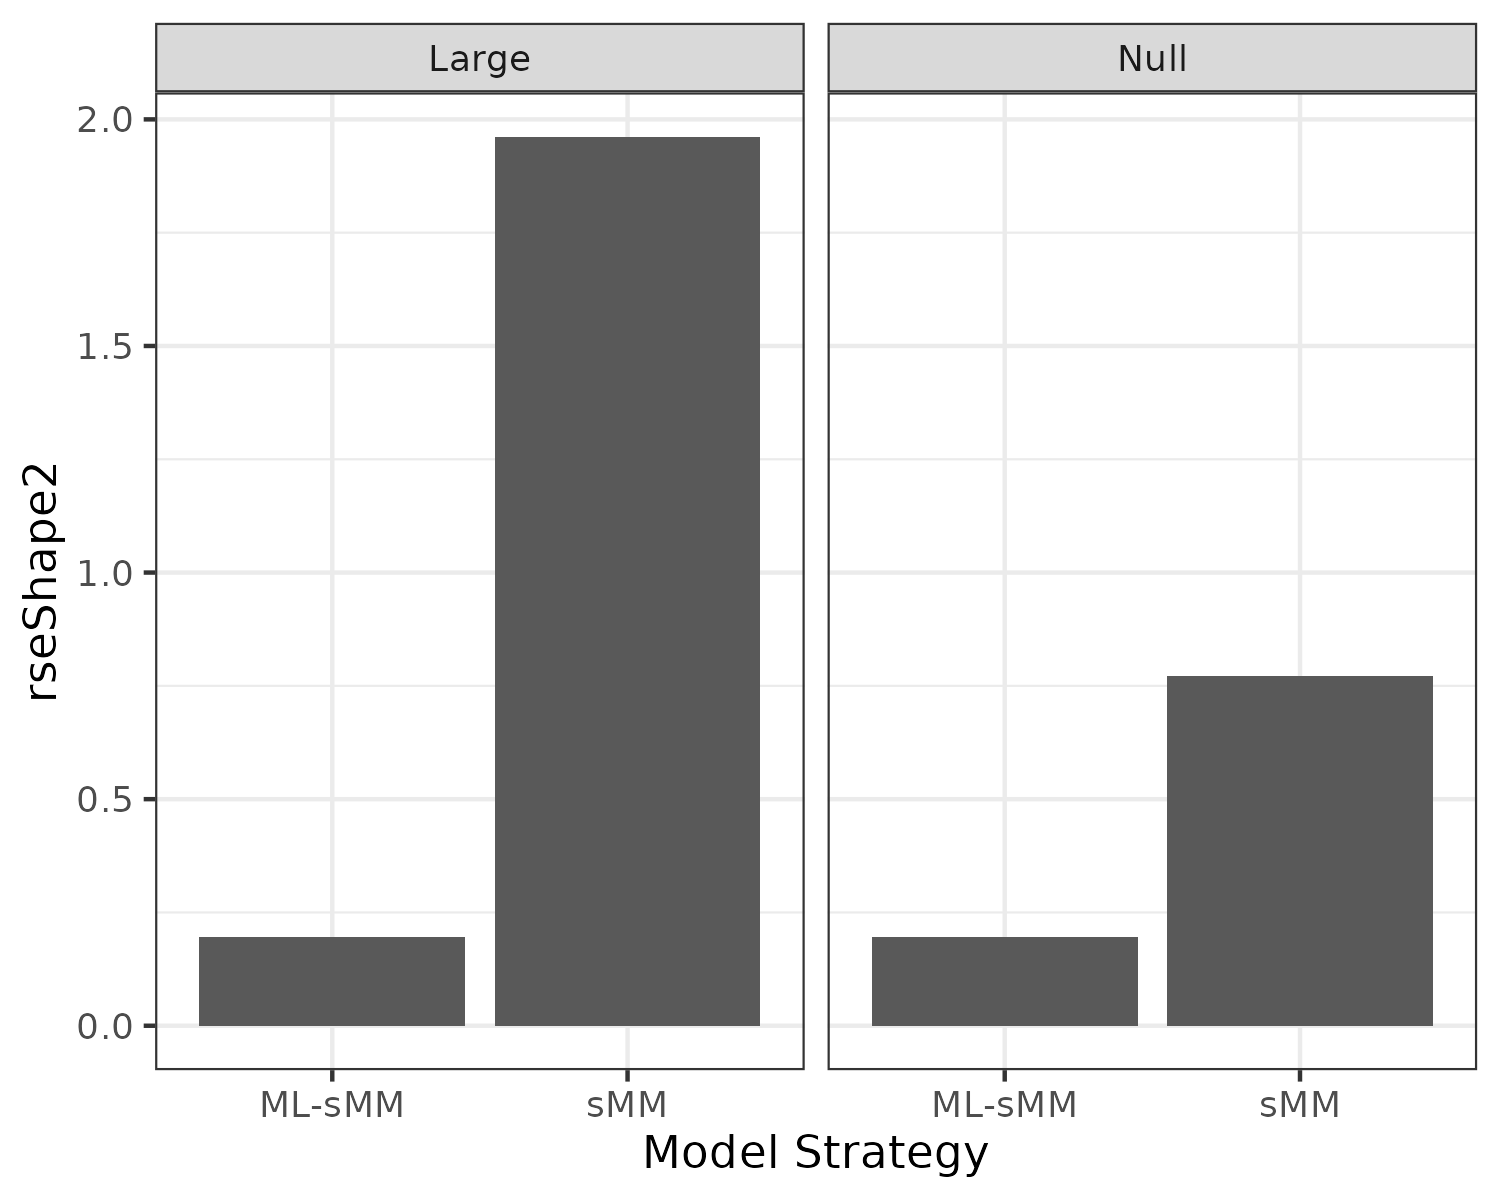
\includegraphics[width=12cm]{figures/anova2TwoWay1.png}
\caption{Two-way interaction from an ANOVA examining differences between
the true and estimate shape parameters}
\end{figure}


\subsection{Parameter Estimation Error and Shape Estimation Error Relationship}
The next examination is an ANCOVA examining the influence of shape
parameter error on criterion variable estimation. This set of analyses
focuses on when shape parameters do not agree, what does this due to
criterion variable estimation. An ANCOVA was estimated including all
prior terms that were included tin the previous ANOVA models and an
additional continuous variable which captures the shape error for a
specific model. Any variables in the ANCOVA model that include the shape
error in them and had an \(\eta^2\) greater than 0.01 were examined (see
table 2.4).

The largest \(\eta^2\) was for the main effect for shape error
(\(\eta^2\) = 0.12), the effect indicated that as shape error increased,
the error when estimating the criterion variable also increased (see
figure 2.7A).

There were two other terms with an \(\eta^2\) greater than 0.01, these
included the interaction between the shape error and the true population
shape term (\(\eta^2 = 0.04\); see figure 2.7B), and the interaction
between the shape error with the sample size (\(\eta^2=0.02\), see
figure 2.7C). The first interaction suggests that shape error increases
criterion variable estimation error much more rapidly when the true
shape parameter was equal to one, while criterion estimation error
increased at a much slower rate when the true population shape term was
greater than one. The second interaction suggests that shape parameter
misestimation poses a much more dangerous threat when the sample size is
smaller.


\begin{table}
    \centering
    \begin{tabular}{cc}
        Parameter & \(\eta^2\) \\
        Shape Error & .12 \\
        Shape Error:Shape Value & .04 \\
        Shape Error:Sample Size & .02\\
        Shape Error:Model Strategy & .01\\
        Shape Error:Shape Value:Sample Size & .01\\
    \end{tabular}
    \caption{Effect sizes examining the influence of shape error on
criterion variable parameter estimation error}
    \label{tab:my_label}
\end{table}

\begin{figure}
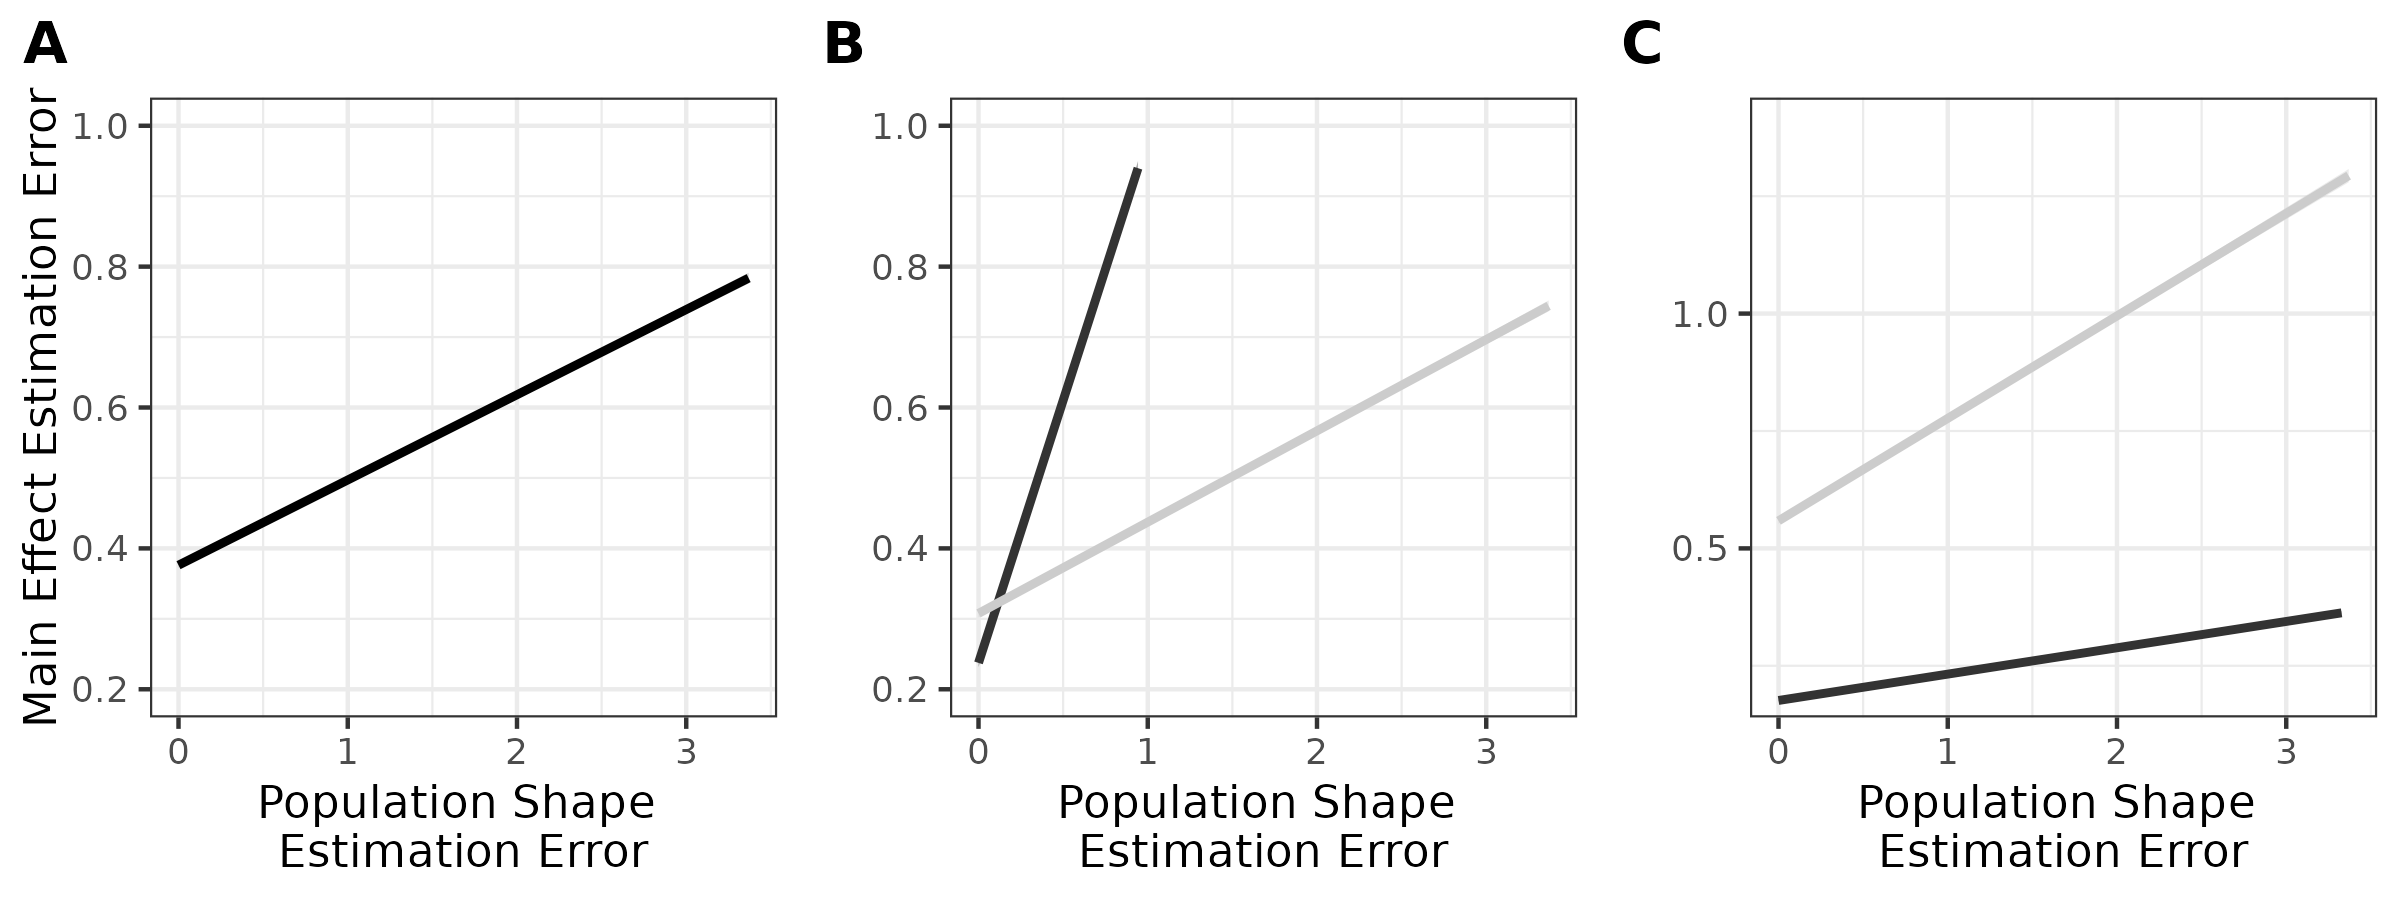
\includegraphics[width=12cm]{figures/shapeEstimationError.png}
\caption{Parameter estimation error regressed onto shape estimation
error main effect and two-way interaction.}
\end{figure}


\subsection{Main Effect Coverage}\label{main-effect-coverage}
The final set of analyses examine the capabilities for the model to
capture the true criterion variable within the 95\%-BCI estimated. For
example, when the data were simulated with a true population criterion
variable parameter of 0, the model assess if 0 is within the lower and
upper 95\%-BCI range. When the true criterion variable was equal to 0.8,
the coverage also examined if 0 was within the 95\%-BCI. So if the
95\%-BCI was below 0 and greater than .8, this was not included as
successfully covering the true population parameter.

To begin with, the main effects of the generalized linear model, the
coefficients and odds-rations of the main effects are listed (see table
2.5) and displayed (see figure 2.8). The effect with largest Odds for
successfully covering the criterion variable's true effect was the
sample size, when increasing the sample size then odds are 2.00 times
more likely to capture the true parameter. The next best thing to
capture the parameter would be the modeling strategy, the multilevel
exponential and Weibull model had similar odds-ratios
(\(OR_{exponential}=1.76; OR_{Weibull}=1.74\)) when compared to a fixed
effect Weibull regression approach.

\begin{table}
\centering
\caption{\label{tab:print-GLM-table}Effect sizes for GLM examining criterion variable parameter coverage}
\centering
\begin{tabular}[t]{l|r|r}
\hline
Parameters & Estimate & OR\\
\hline
Intercept & 2.07 & 7.92\\
\hline
Large Sample Size & 0.70 & 2.01\\
\hline
Long Minimum Observation & -0.26 & 0.77\\
\hline
Random Emission Pattern & 0.00 & 1.00\\
\hline
Long Scale Values & 0.01 & 1.01\\
\hline
Weibull Shape Parameter & -0.20 & 0.81\\
\hline
Large Main Effect & -1.67 & 0.19\\
\hline
Large Random Variance & -0.65 & 0.52\\
\hline
ML-sMM & 0.56 & 1.75\\
\hline
MM & -0.16 & 0.85\\
\hline
ML-MM & 0.57 & 1.77\\
\hline
\end{tabular}
\end{table}

\begin{figure}
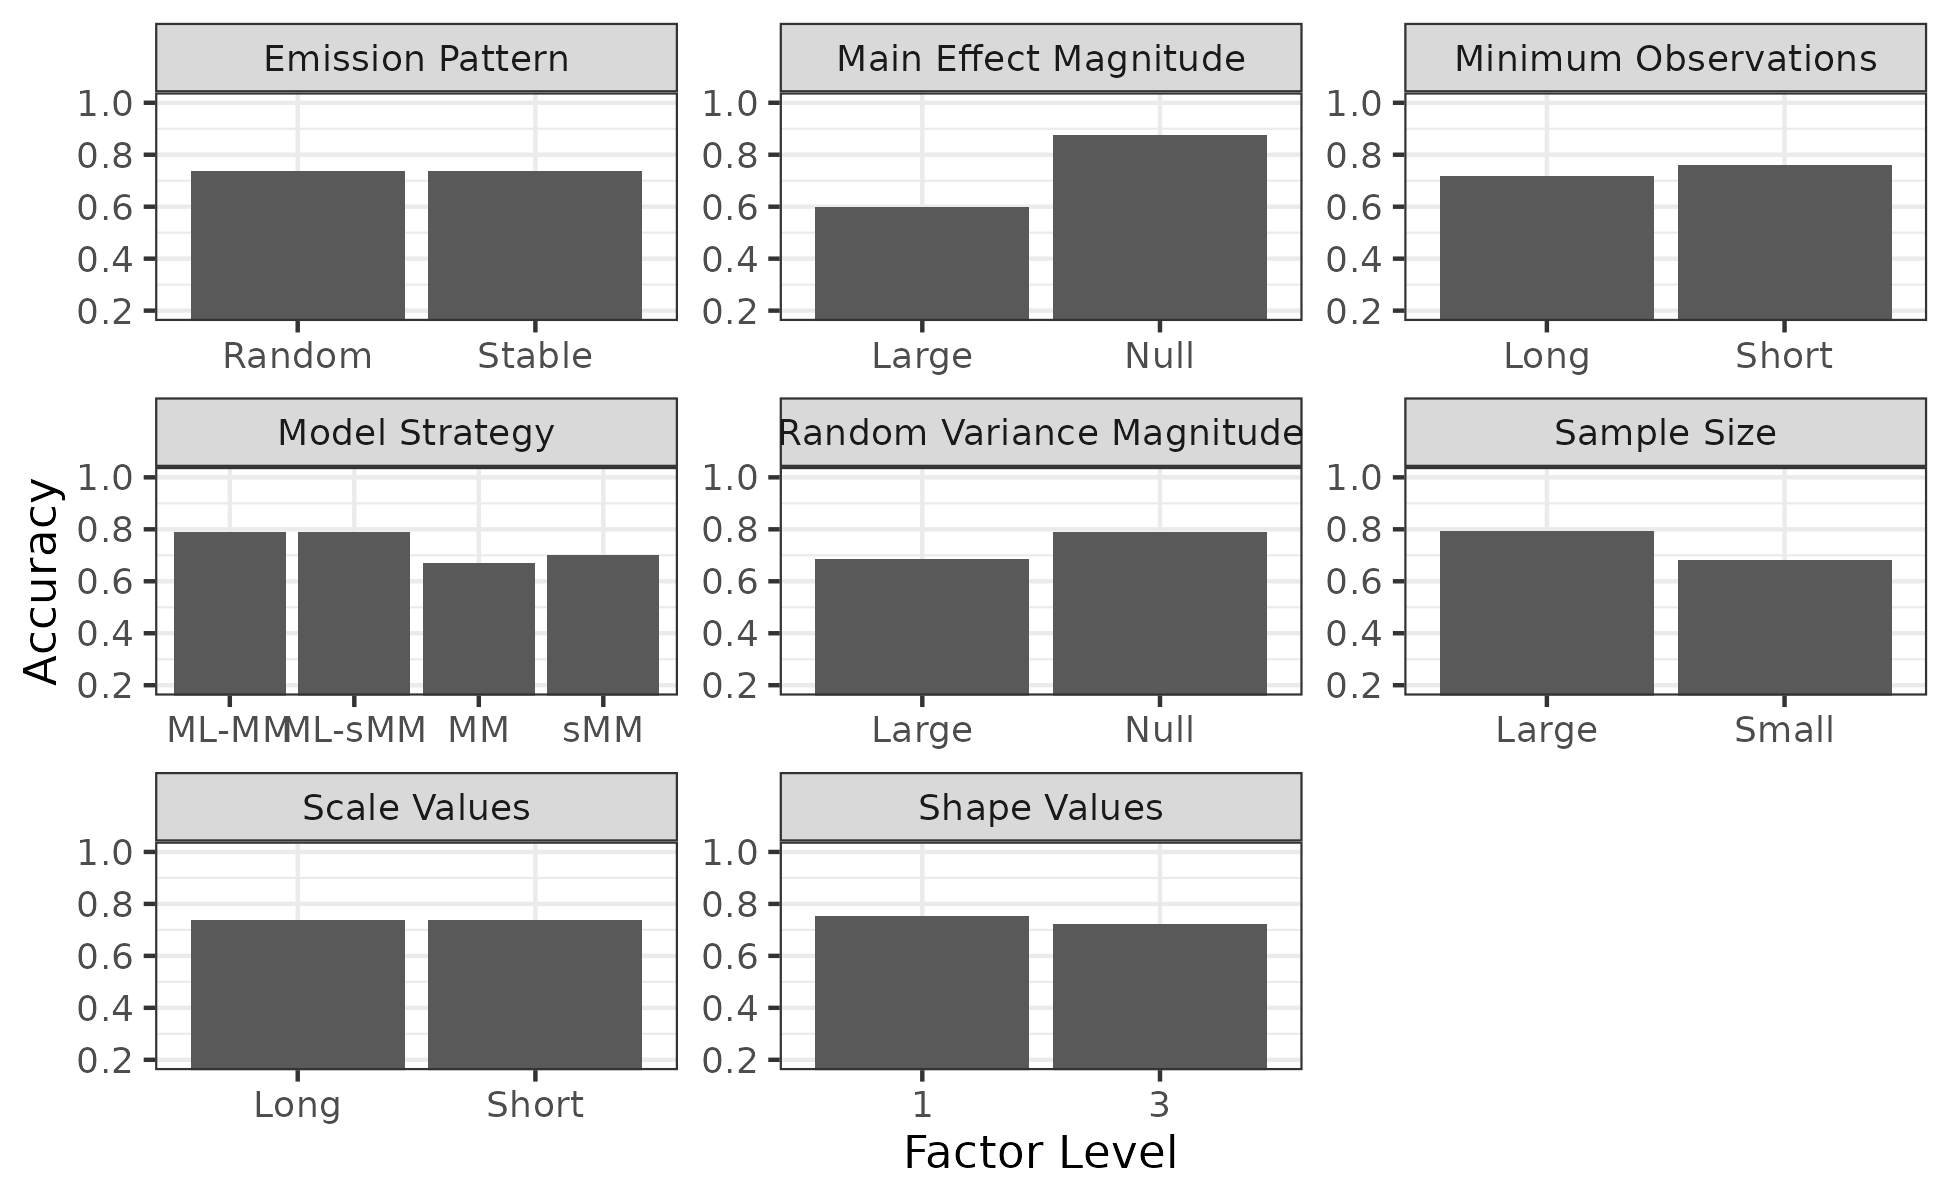
\includegraphics{figures/glm1MainEffect.png}
\caption{Proportion of correct identifications for all main effects in
GLM predicting correct classification of true population effect}
\end{figure}

The examination of the two-way interactions was focused on interactions
including modeling strategy. The interaction between the magnitude of
the random variance and the modeling strategy displays how poorly the
fixed effect approach perform when compared to the multilevel
alternatives (see figure 2.9). For example, when random variance is
large, the fixed effect exponential model correctly captures the true
criterion variable's effect 55\% of the occasions; whereas, the
multilevel alternative captures the true effect more than 75\% of the
time. When random variance was not present, performance across all
modeling types was much more consistent with accuracy ranging from .8 to
.75, with the most accurate being the multilevel exponential model, and
the least accurate being the fixed effect Weibull approach. The next
two-way interaction which merited discussion was the interaction between
the sample size and the modeling approach (see figure 2.10). The
interaction was driven by superior performance of the multilevel
modeling techniques across both sample size permutations, although
performance was higher across all techniques when sample sizes were
larger.

\begin{figure}
\centering
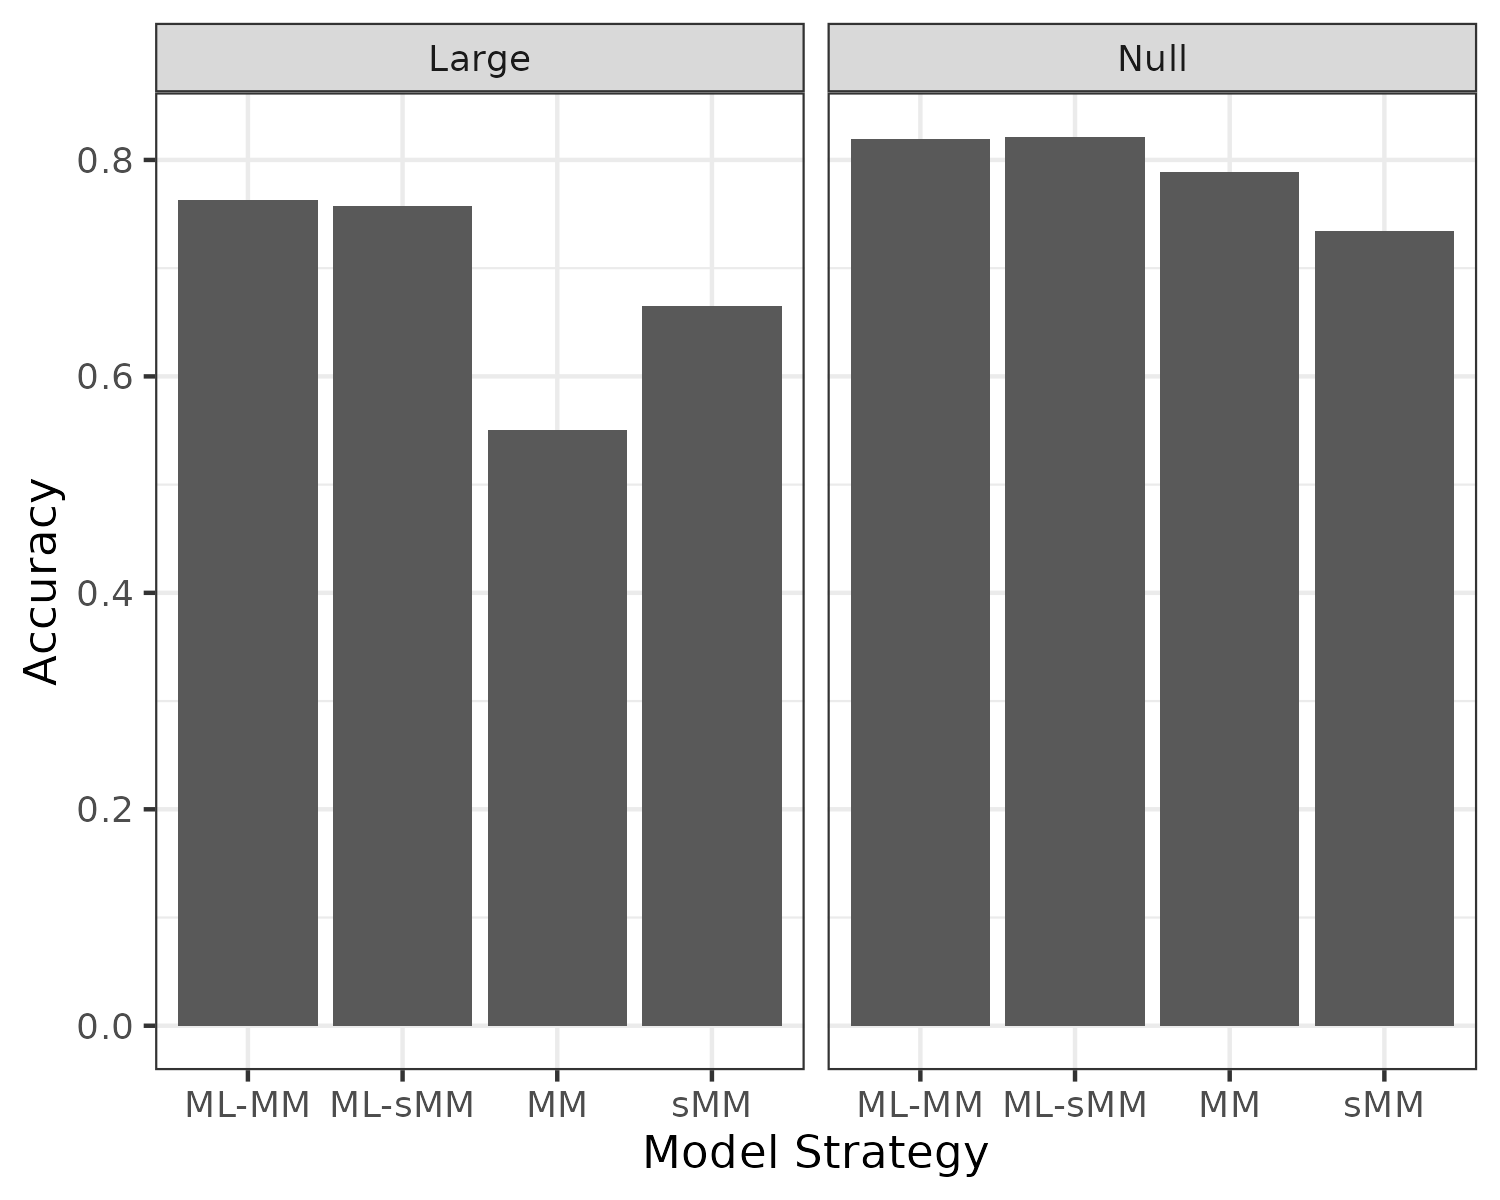
\includegraphics{figures/glm1TwoWay1.png}
\caption{Two-way interaction examining identification accuracy for the
population fixed effect across all modeling strategies with and without
random variance}
\end{figure}

\begin{figure}
\centering
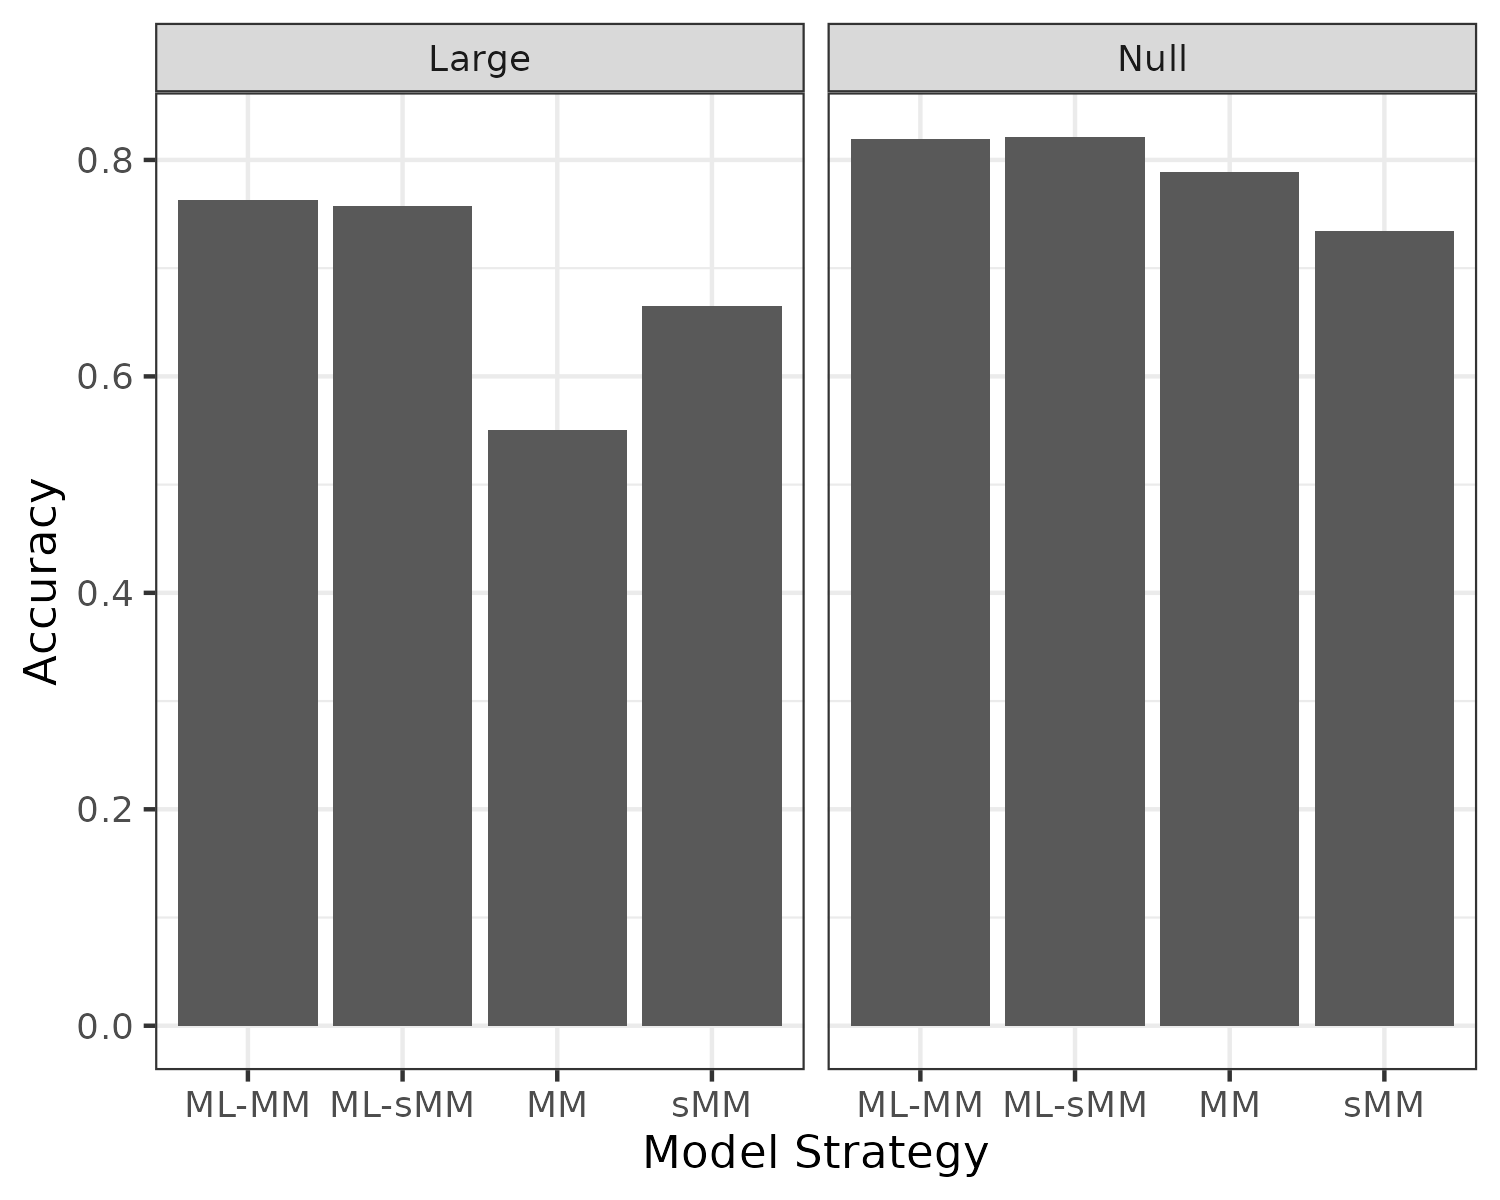
\includegraphics{figures/glm1TwoWay2.png}
\caption{Two-way interaction examining identification accuracy for the
criterion variable across modeling strategy and sample size}
\end{figure}

\newpage

\section{Discussion}\label{discussion}

The major motivation of this simulation was to examine how flexible is
the continuous-time Markov model when data do not adhere to the
memoryless assumption applied in the model. This question was further
compounded with pooling information from a homogeneous and heterogeneous
populations as assessed the magnitude of random effect variance.
Performance of four separate modeling techniques was assessed across
three separate analyses. The results offered convergent results
describing when a model is constrained to include the memoryless
assumption (i.e.~exponential distribution) and as random variance
increases, not accounting for either of these increases criterion
variable estimation error.

The first ANOVA examined the distance from a model estimated criterion
variable and the population's true effect. The biggest predictor of
estimation error was the presence of random variance. Specifically, when
data were simulated with a participant specific sampled from a normal
distribution with a variance of 1 this presence or lack thereof,
explained roughly 30\% of the error between the true and estimated
parameters. While the shape parameter used to generate the data did not
display a strong effect size from this model the next two set of
analyses specifically address shape mismatch between generated and
estimated model. One of the best steps taken to reduce the error was
identified by the model estimation strategy, which explained only
roughly 5\% of the total variance, but in the anticipated direction.
Specially error was lower when models were estimated including a random
effect in the estimation, and even lower when the model was estimated
assuming the data were generated from a Weibull distribution, across
even wen they were generated from an exponential distribution.
Furthermore, the multilevel models displayed equivalent levels of
estimation error when no random effect was present in the data,
indicating that estimating the model via a Bayesian multilevel model
potentially offers no drawbacks in this simulation study.

The second model examines the capabilities of the Weibull regressions to
estimate the true population shape's parameter. The exponential
distribution models were excluded from these analyses as the shape
parameter is fixed, at least when translating a Weibull into an
exponential distribution. These models examine the factors that
contribute to difficulties when identifying the true shape parameter,
the largest effect size was unsurprisingly if the data were generated
with a shape parameter equal to or greater than 1. The shape parameter
becomes much more difficult to estimate when the true value is greater
than one. Consistent with the previous set of analyses, estimation error
also increased when random variance was introduced into the model.
Again, consistent with the previous set of analyses, the multilevel
Weibull model (i.e.~the multilevel semi-Markov model) performed the best
at recovering the true shape parameter.

The importance the model to recover the shape parameter is underscored
by the ANCOVA. The ANOCVOA examines the relationship between the
criterion variable estimation error and shape parameter mismatch. There
is a strong positive relationship between these two variables, in fact
the ANCOVA suggests that more than 10\% of the error in the criterion
variable can be explained by the shape parameter error. These analyses
were constrained to both the multilevel and the fixed effect Weibull
analyses. The exponential regression is equivalent to a Weibull
regression with a shape parameter of 1, had these models been included
in these analyses the estimation error would have either been 0 or 2;
while the no shape estimation error is excellent, the error of 2 is
larger than the majority of observed differences between true and
estimated shape parameters.

Finally, the last analysis examined the coverage of the true parameter
effect via a logistic regression. Coverage was classified as identifying
0 within the 95\%-BCI when the true parameter was 0 or having the true
parameter effect of 0.8 and excluding 0 in the 95\%-BCI. This framework
was set up to mimic recommended practices when applying a Bayesian
modeling framework (Kruschke \& Liddell, 2018). The results of the model
clearly indicate superior performance when a multilevel framework is
applied. Classification accuracy remained consistently around 80\% for
both the multilevel exponential and multilevel Weibull models when
estimated with and without true population random variance. While the
fixed effect counterparts accuracy plummeted to as low as 55\%. When
these models were estimated without any random variance, performance
across all models improved, however, the multilevel models still had
better accuracy values. What this suggests for the applied researchers
is that there seems to be little to no risk of applying a multilevel
framework for estimating time-to-event analyses. Of course, this is in
stark contrast to some of the published literature that examines the
utility of frailty models. The criticisms surrounding the application of
frailty models examines issues in identifying the model with complex
multistate analyses (Putter \& van Houwelingen, 2015). Here, a total of
554 models did not converge at an acceptable level representing less
than 0.001\% of estimated models. Suggesting that the Bayesian sampling
criteria applied to estimate these models may reduce these such
concerns. It is worth stating that these previous concerns were made
when estimating the multi-state frailty models for panel data; whereas,
the application of these models were to intensive longitudinal data,
which may reduce the potential concern of model identification.

This simulation puts forward a compelling narrative for the application
of the multilevel Weibull model when estimating time-to-event data. This
suggestion is even stronger when there is potential for intra-cluster
correlation for timing of the outcomes of interest. Studies which
examine dyadic interactions are certainly vulnerable to these such
dyadic specific variance. This is why the applied study in the next
section is a strong candidate for the multilevel Weibull model that is
applied.


\chapter{Dynamics of Verbal Parental Actions During A Structured Cleaning Task}\label{chap:Emp} 
\section{Introduction}
Parent-child interactions have been a mainstay in psychological research
for decades. Such topics date back to the invention of talk based
therapy paradigms such as psychoanalysis as developed by Freud (Freud,
1910). More recently psychology has focused on the quality of the
relationship between an infant and their caregiver such as those
assessed by the strange situation paradigm (Ainsworth et al., 1978).
Now, contemporary treatment paradigms are seeking to structure this
relationship to improve parent-child relationships. By structuring the
disciplinary and reinforcement practices between a parent-child dyad,
Parent-Child Interaction Therapy (PCIT; S. Eyberg (1988)), seeks to
improve the bonds between a child and their caregiver.

The foundation of PCIT is born out of fields such as social learning,
attachment theory, and family systems theory (E. A. Skowron et al.,
2024). Early applications of PCIT were focused on treating externalizing
and oppositional disorders in children (Cooley et al., 2014). The
structure of PCIT involves ``coaching'' a parent through various types
of interactions with their child. The coaching is performed by a trained
therapist. Throughout the administration, parent-child interactions are
observed by the therapist, the parent wears a microphone so they can
listen to instructions from the therapist. Through this mechanism, the
therapist is capable of coaching the parent through various situations
they may face during these therapy sessions. The administration of PCIT
has two distinct stages which either focus on child directed or parent
directed interactions. The child directed stage is focused on developing
positive interactions between the parent and the child. Mastery of the
child directed stage is assessed by the frequency of these positive
practices expressed over a 5-minute play session. Parents are instructed
to allow the child to lead play sessions and the parent is instructed to
encourage and praise their child when appropriate. The parent directed
stage involves teaching the parent safe and effective strategies to
discipline their child when children are misbehaving or ignoring their
parent. Mastery of the parent directed stage involves the ability for
the parent to enforce these disciplinary practices (Eyberg et al., 2014;
Funderburk \& Eyberg, 2011).

Several tasks and outcomes exist which can be used to measure the
efficacy of PCIT. The dyadic parent-child interactions interactions
coding system (DPICS; Eyberg et al. (2014)) provides a fairly uniform
process to analyze the mastery of PCIT. The DPICs is a structured task
that is composed of 3 5-minute blocks where the parent and child are
recorded during a laboratory setting session. The first 5-minute session
is child-led play, where the parent is instructed to allow the child to
guide what the dyad will be doing. The next is a 5-minute parent-led
play session, where the parent leads the child in play for 5
minutes. Finally, the last session is a 5-minute clean-up task, where
the parent instructs the child to clean up the room. The goal of the
clean-up task is to simulate a frustrating situation for both the parent
and child, and to observe and code the parent's behavior, and if the
child complies with the parents commands. Beyond the actual laboratory
session, the DPICs also provides a coding framework which assigns
parental actions into one of three distinct and nonoverlapping
categories. These categories include PRIDE, neutral, DON'T actions. As
the goal of PCIT is to increase the frequency of positive (i.e.~PRIDE)
interactions, and decrease the frequency of negative (i.e.~DON'T)
actions the DPICs provides a structured setting to assess the frequency
of these behaviors. The specifics of these verbal coding classifications are further
expanded upon in the methods section of this chapter. This task was
developed specifically for PCIT, the DPICS system is highly sensitive to
behaviors that are coached in PCIT and other behavioral parent training
programs (Nelson \& Olsen, 2018).

Historically, the analyses of the DPICs task have focused on the
frequency of parental verbal interactions (Eyberg et al., 2014). These
frequencies typically capture the total number of PRIDE, neutral, and
DON'T verbal actions, and the child's compliance to commands. Either the
ratio or tallies of these behaviors will then be used as a criterion
variables to assess PCIT treatment effects. Such practices have long
been the analytic paradigm for DPICs studies, for example these tallies
have been used to estimate factor scores (Cañas et al., 2022), examine
the efficacy of PCIT intervention (Abrahamse et al., 2016; Bjørseth \&
Wichstrøm, 2016; Cooley et al., 2014), and to assess the psychometric
properties of the DPICs (Cañas et al., 2020; Gridley et al., 2018).
Analyzing the outcomes in this manner of course ignores how richly the
data are coded in terms of what and when an action occurs. Recent steps
have been taken to analyze the DPICs via incorporation when and how much
of parental actions are performed.

Temporal analyses of the DPICs task have been a relatively recent
methodological pursuit. Examples of these analyses specific to the DPICs
include applications of both discrete-time dynamic structural equation
modeling (Somers et al., 2024), and a hidden Markov model based approach
(Lunkenheimer et al., 2017). The former deviates from the current study
because data are collapsed into specific length epochs. The application
of the discrete-time structural equation modeling as applied by Somers
et al., required assigning all actions taken within 10-second epochs,
and using these as a multivariate streams of data. This work allowed the
authors to examine dynamic relationships between the parent's harsh
behavior and the child's compliance across and within epochs. The work
by Lunkenheimer et al., did use data from the DPICs analyses, but
included data beyond the coding of the parent's verbal exchanges. The
parents had streams of multiple behaviors including positive behaviors
such as: directive, positive reinforcement, engagement, and emotional
support behaviors, as well as negative behaviors which included:
off-task disengagement, intrusion, and negative discipline. While these
data may be available to any video-recorded DPICs assessment, they go
beyond the simple coding structure that is inherent to both that PCIT
and DPICs share. These data were coded into 1-second epochs, and a
hidden Markov model was used to identify transition between engaged and
unengaged states across dyads.

The goal of this study is to examine verbal dynamics of parents during
the DPICs study and how the administration of PCIT influences these
dynamics. Parents who are at high risk of abuse or neglect were
recruited and pre- and post-PCIT DPCIS administrations were used to
examine differences in verbal interactions following the administration
of PCIT. Furthermore, we also seek to incorporate the child's compliance
behavior and to examine how this influences the parents behavior. These
set of analyses seek to incorporate the minimally coded DPICs analyses
but incorporates the richness of the temporal aspects of these data to
examine the dynamic behaviors.   

\section{Methods}
The goal of this study was to examine how PCIT therapy influences
parent-child interactions during the administration of the DPICS task.
The tasks required to examine this goal are described below, briefly
this required, recruiting participants who were at high-risk for abuse
or neglect of their children, administer a pre-treatment DPICs session,
assign participants to either a case or intervention cohort, administer
the PCIT therapy or service-as-usual (SAU), and then administer a
post-treatment DPICs. The DPICs data were coded for every verbal
interaction the parent had with their child, and these verbal
interactions were the unit of analysis for all semi-Markov models. The
semi-Markov models examined the timing and type of interaction a parent
had with their child during the clean-up task of the DPICs task. These
interactions were then analyzed using a multilevel Weibull regression
model. These steps are further expanded upon below.

\subsection{Participants}
Parents and their 3--7-year-old children were recruited from the Oregon
Department of Human Services (DHS) child welfare and self-sufficiency
units. Prospective families completed an initial phone screen with a
research recruiter who introduced the study and inclusion criteria, as
follows: 1) parent is 18+ years old at study entry and 2) is the
participating child's biological or custodial caregiver; 3)
participating child is 3 to 7 years old; 4) parent and child were living
together at least 50\% time; 5) both spoke English. Parents with a
history of perpetrating child sexual abuse were excluded along with
their children due to contraindications for PCIT services. Further
information on the clinical trial's recruitment procedures is available
in the study protocol (Nekkanti et al., 2020; E. Skowron, 2023). The
study employed a parallel group design, in which families were
randomized to PCIT intervention or DHS services-as-usual (SAU) control
conditions, blocked by child sex and age. An allocation ratio of 1.5:1
to intervention and control conditions helped to ensure sufficient
families were randomized to intervention. Allocation was concealed from
research assistants who conducted the assessments. Of 228 families
scheduled for an intake, 204 parent-child dyads completed pretreatment
assessments and were randomized to condition: PCIT intervention group; n
= 120; and SAU control group; n = 84. Sample size was determined based
on Monte Carlo simulations using Mplus (Linda K., Muthén \& Bengt O.,
Muthén, 2017) to enable detection of small intervention effects and
small-to-moderate mediation effects with estimated power greater than
0.80. At study entry, parents were between ages 18 and 64 (M = 32.32, SD
= 6.38) and were predominantly mothers (n=180). The majority (98\%) of
participating parents were biological parents of their child. Less than
half (46.3\%) of parents were employed, and 78.5\% of households were
living below the federal poverty line based on 2020 U.S. Department of
Health and Human Services guidelines. A majority (73.5\%) of parents had
experienced 4 or more Adverse Childhood Experiences (ACEs M = 5.24, SD =
2.69) themselves. Participating children were 3-7 years of age (M =4.76,
SD = 1.40 years) with the exception of one child who turned 8 years-old
a few days before a canceled assessment was rescheduled. A majority
(69.1\%) of children had experienced 3 or more ACEs at study entry. Only
one-third (34.8\%) of parents reported elevated Eyberg Child Behavior
Inventory (Eyberg \& Robinson, 1983) behavior problems. Regarding the
adequacy of randomization, no significant differences were observed
across conditions on any pretreatment variables except marital status
(38\% of parents were married or living together in the PCIT condition
versus 24\% in the control group).

The sample was drawn from consecutive family referrals received between
April 2016 and June 2019 from the Department of Human Services-Child
Welfare and Self-Sufficiency, and who consented to enroll in the study.
The study was registered with clinical trials.gov (Coaching Alternative
Parenting Strategies Study; NCT02684903) and procedures were approved by
the Institutional Review Board. Written informed consent was obtained
from participating parents and the family's caseworker in cases where
the Department of Human Services maintained legal custody of the child
while parents retained physical custody. Children and their parents in
both conditions completed identical pre- and post-intervention
assessments. The majority of enrolled families in the control group
(81\%) and PCIT intervention condition (83\%) completed the
post-treatment assessments, which were conducted on the same timeline
across the conditions (i.e., M=7.8, SD=2.3 months post-study entry).
Families were compensated for attending assessments, reimbursed for
transportation costs, and received refreshments, rest breaks, and
childcare for non-participating children. Participating children
received a small prize.

\subsection{DPICS Dyadic Interaction Task}\label{dpics-dyadic-interaction-task}
Using a standardized set of toys distributed across the playroom table
and floor, child and parent dyads completed a series of three 5-min
interaction tasks. In the Child-Led Play task, parents were instructed
to let their child decide what to play with and follow their child's
lead in the play. Next during the Parent-Led play task, parents were
instructed to choose the play activity. In the final task, Toy
Clean-Up, parents were instructed to direct their child to clean up all
of the toys by themselves. Digital video-recording enabled offline
transcription and behavioral coding via the Dyadic Parent-Child
Interaction Coding System-IV (DPICS-IV; S. Eyberg (1988); see below).
Parental verbal actions were coded into one of several distinct and non
overlapping categories (see table 3.1). The timing of each of these
behaviors and these specific states composed an individual's data stream
(see figure 3.1A\&B for an example).

\begin{table}
    \centering
    \begin{tabular}{cc}
        Action State & Verbal Classification\\
        Pride & Compliable Commands, Behavior Description, Praise, Reflection \\
        Neutral & Neutral Talk, Questions \\
        Don't & Negative Talk, Non-Compliable Commands \\
    \end{tabular}
    \caption{DPICs Verbal coding actions for Clean-up task}
    \label{tab:my_label}
\end{table}


\begin{figure}
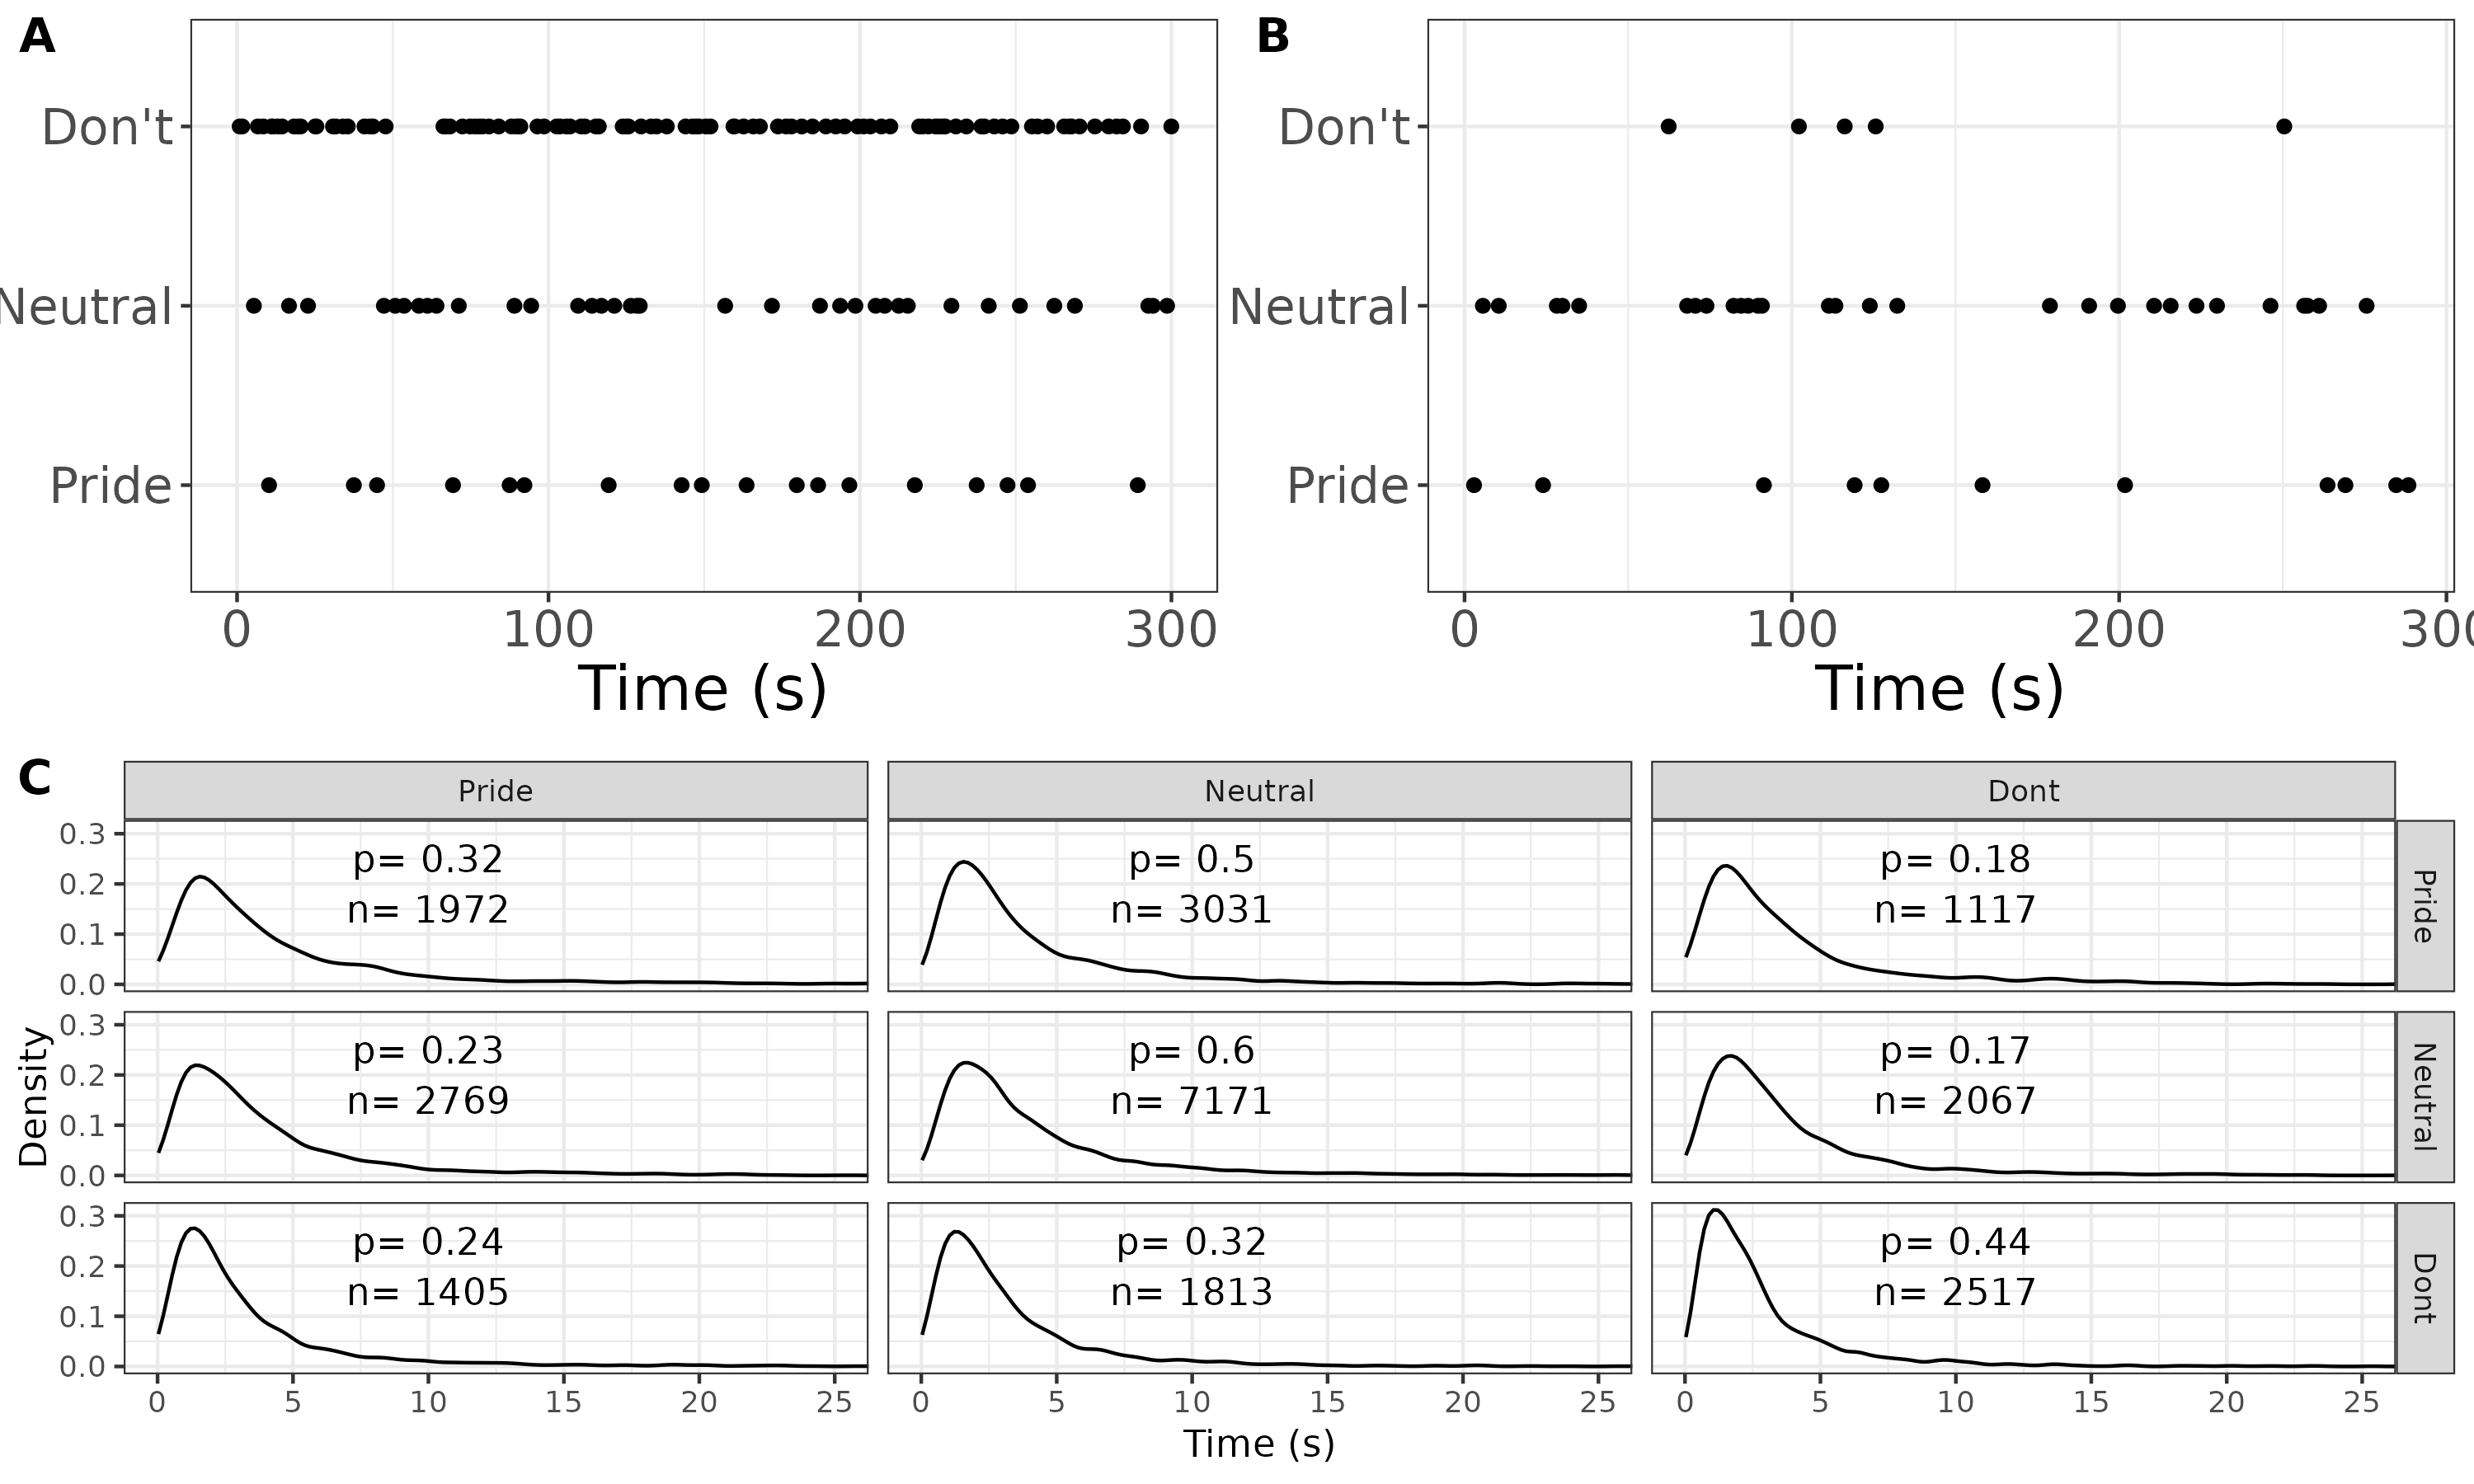
\includegraphics[width=12cm]{figures/CLUPTimeSeries.png}
\caption{Comparing the most active dyad during the clean-up task with
the most passive active dyad}
\end{figure}

\subsection{Modeling}\label{modeling}

In order to model transition dynamics the time between specific state
emissions were modeled using a continuous-time semi-Markov model
parameterized via a multilevel Weibull regression. The multilevel
framework was applied given the qualitative differences observed in the
frequency of verbal actions within specific dyads (see figure 3.1 A\&B).
This required regressing the sojourn times for specific state
transitions (see figure 3.1C) onto specific criterion variables. The
criterion variables included if an assessment was performed at a pre- or
post-intervention assessment, if the participant was assigned to the SAU
group or the intervention group, and the specific transition type. All
of these analyses follow an intent-to-treat paradigm such that for any
dyad assigned to the intervention cohort, even if they did not receive
any PCIT sessions, they were coded as the intervention group. All
variables and up to all three-way interactions were included.

The next model examines how the compliance from the child influences the
parents verbal actions. This required estimating an additional model
because compliance is only possible following a compliable command which
is coded as a PRIDE action. Thus, these terms could not be included when
all possible interactions were explored because the transitions out of
the neutral and DON'T states can not interact with compliance. In order
to examine the influence that compliance has on parent's actions,
sojourn times following all compliable commands were regressed onto the
same criterion variables as in the previous model plus an additional
variable detailing if the child complied with the command.

Models were estimated using a Bayesian framework. A total of 10,000
samples were performed with a burn-in length of 2,000 samples. Chains
were thinned by including every 10\textsuperscript{th} estimated sample. A total of 6
chains were estimated. The sampling was performed using the NUTs
algorithm which is standard to the STAN software (S. D. Team, 2023).
Significant effects were examined via the 95\%-BCI, any four-way or
three-way interaction which did not include 0 in the BCI was further
examined. Interactions were examined both by observing the mean sojourn
time of a state, as well as examining the hazards for a specific
transition, the former informs temporal differences on when transitions
occur, while the latter incorporates transition probabilities the
estimation. All analytic code is available online
\href{https://github.com/adrose/oregonDPICS/blob/main/scripts/brmsSkel.R}{here}.

\section{Results}\label{results-1}

\subsection{All Transition Summary Statistics}
In total, there were 23,862 verbal interactions recorded across all
groups, and waves. The most frequent state was the neutral state with a
total of 12,007 neutral expressions observed. There were a total of
6,120 PRIDE expressions and the most infrequent state was the 5,735
expressions. The quickest emissions were observed within the DON'T into
DON'T state interactions, with a mean sojourn time of 2.7 seconds (see
figure 3.1C). The slowest transitions were observed between the PRIDE
into PRIDE transitions with an average sojourn of 4.5 seconds (see
figure 3.1C).

\subsection{Model Convergence}
Model convergence was assessed using the \(\hat{R}\) statistic as well
as visual assessment of the autocorrelation function within each
parameter's samples. The first examines if the chains had mixed
\(\hat{R}\) values below 1.05 are generally deemed as evidence that
chains have mixed and convergence was obtained. All parameter
\(\hat{R}\) values were less than 1.05, indicating chains mixed well.
The second, visual assessment of the auto correlation functions from the
drawn samples indicates if the sampling procedure was able to
sufficiently examine the parameter space. Autocorrelations with lag's
greater than 1 were all less than .1 suggesting little to no
relationship of prior samples influence future samples. Thus, the
evidence indicates that the Bayesian models converged and were able to
adequately sample the parameter space.

\subsection{Wave by Group Effects Across All Transition Patterns}
The next set of analyses examines both treatment and practice effects.
Practice effects are indicated by a wave by transition-type interaction.
This interaction is controlling for group effects. In total, three
interactions saw a wave effect: the first was the PRIDE into PRIDE
transition (\(\beta=0.14, BCI_{lower}=0.02, BCI_{upper}=0.26\); see
figure 3.2), this suggests that on the second administration of the
DPICs, sojourn times increased for these transitions. The second effect
was observed for the PRIDE into neutral interactions
(\(\beta=-0.21, BCI_{lower}=-0.36, BCI_{upper}=-0.05\)), indicating
emission from the PRIDE state into the neutral state occurred quicker in
the second administration of the DPICS. The last practice effect was
observed for the neutral into neutral interactions
(\(\beta=-0.17, BCI_{lower}=-0.30, BCI_{upper}=-0.03\)) indicating
quicker emissions from neutral into neutral upon readministration of the
DPICS.

The next set of analyses examines the three-way interactions which
examines the PCIT effect on the readministration of the DPICs sojourn
times. Non-zero effects were observed in two transition times when
examining these effects. The transitions from PRIDE into neutral for the
intervention cohort displayed a longer sojourn time compared to the
control cohort at wave 3
(\(\beta=0.13, BCI_{lower}=0.01, BCI_{upper}=0.32\); see figure 3.2). The
second transition for the neutral into DON'T state
(\(\beta=0.10, BCI_{lower}=0.01, BCI_{upper}=0.23\); see figure 3.2),
again indicating a longer transition time for the intervention cohort.

\begin{figure}
\centering
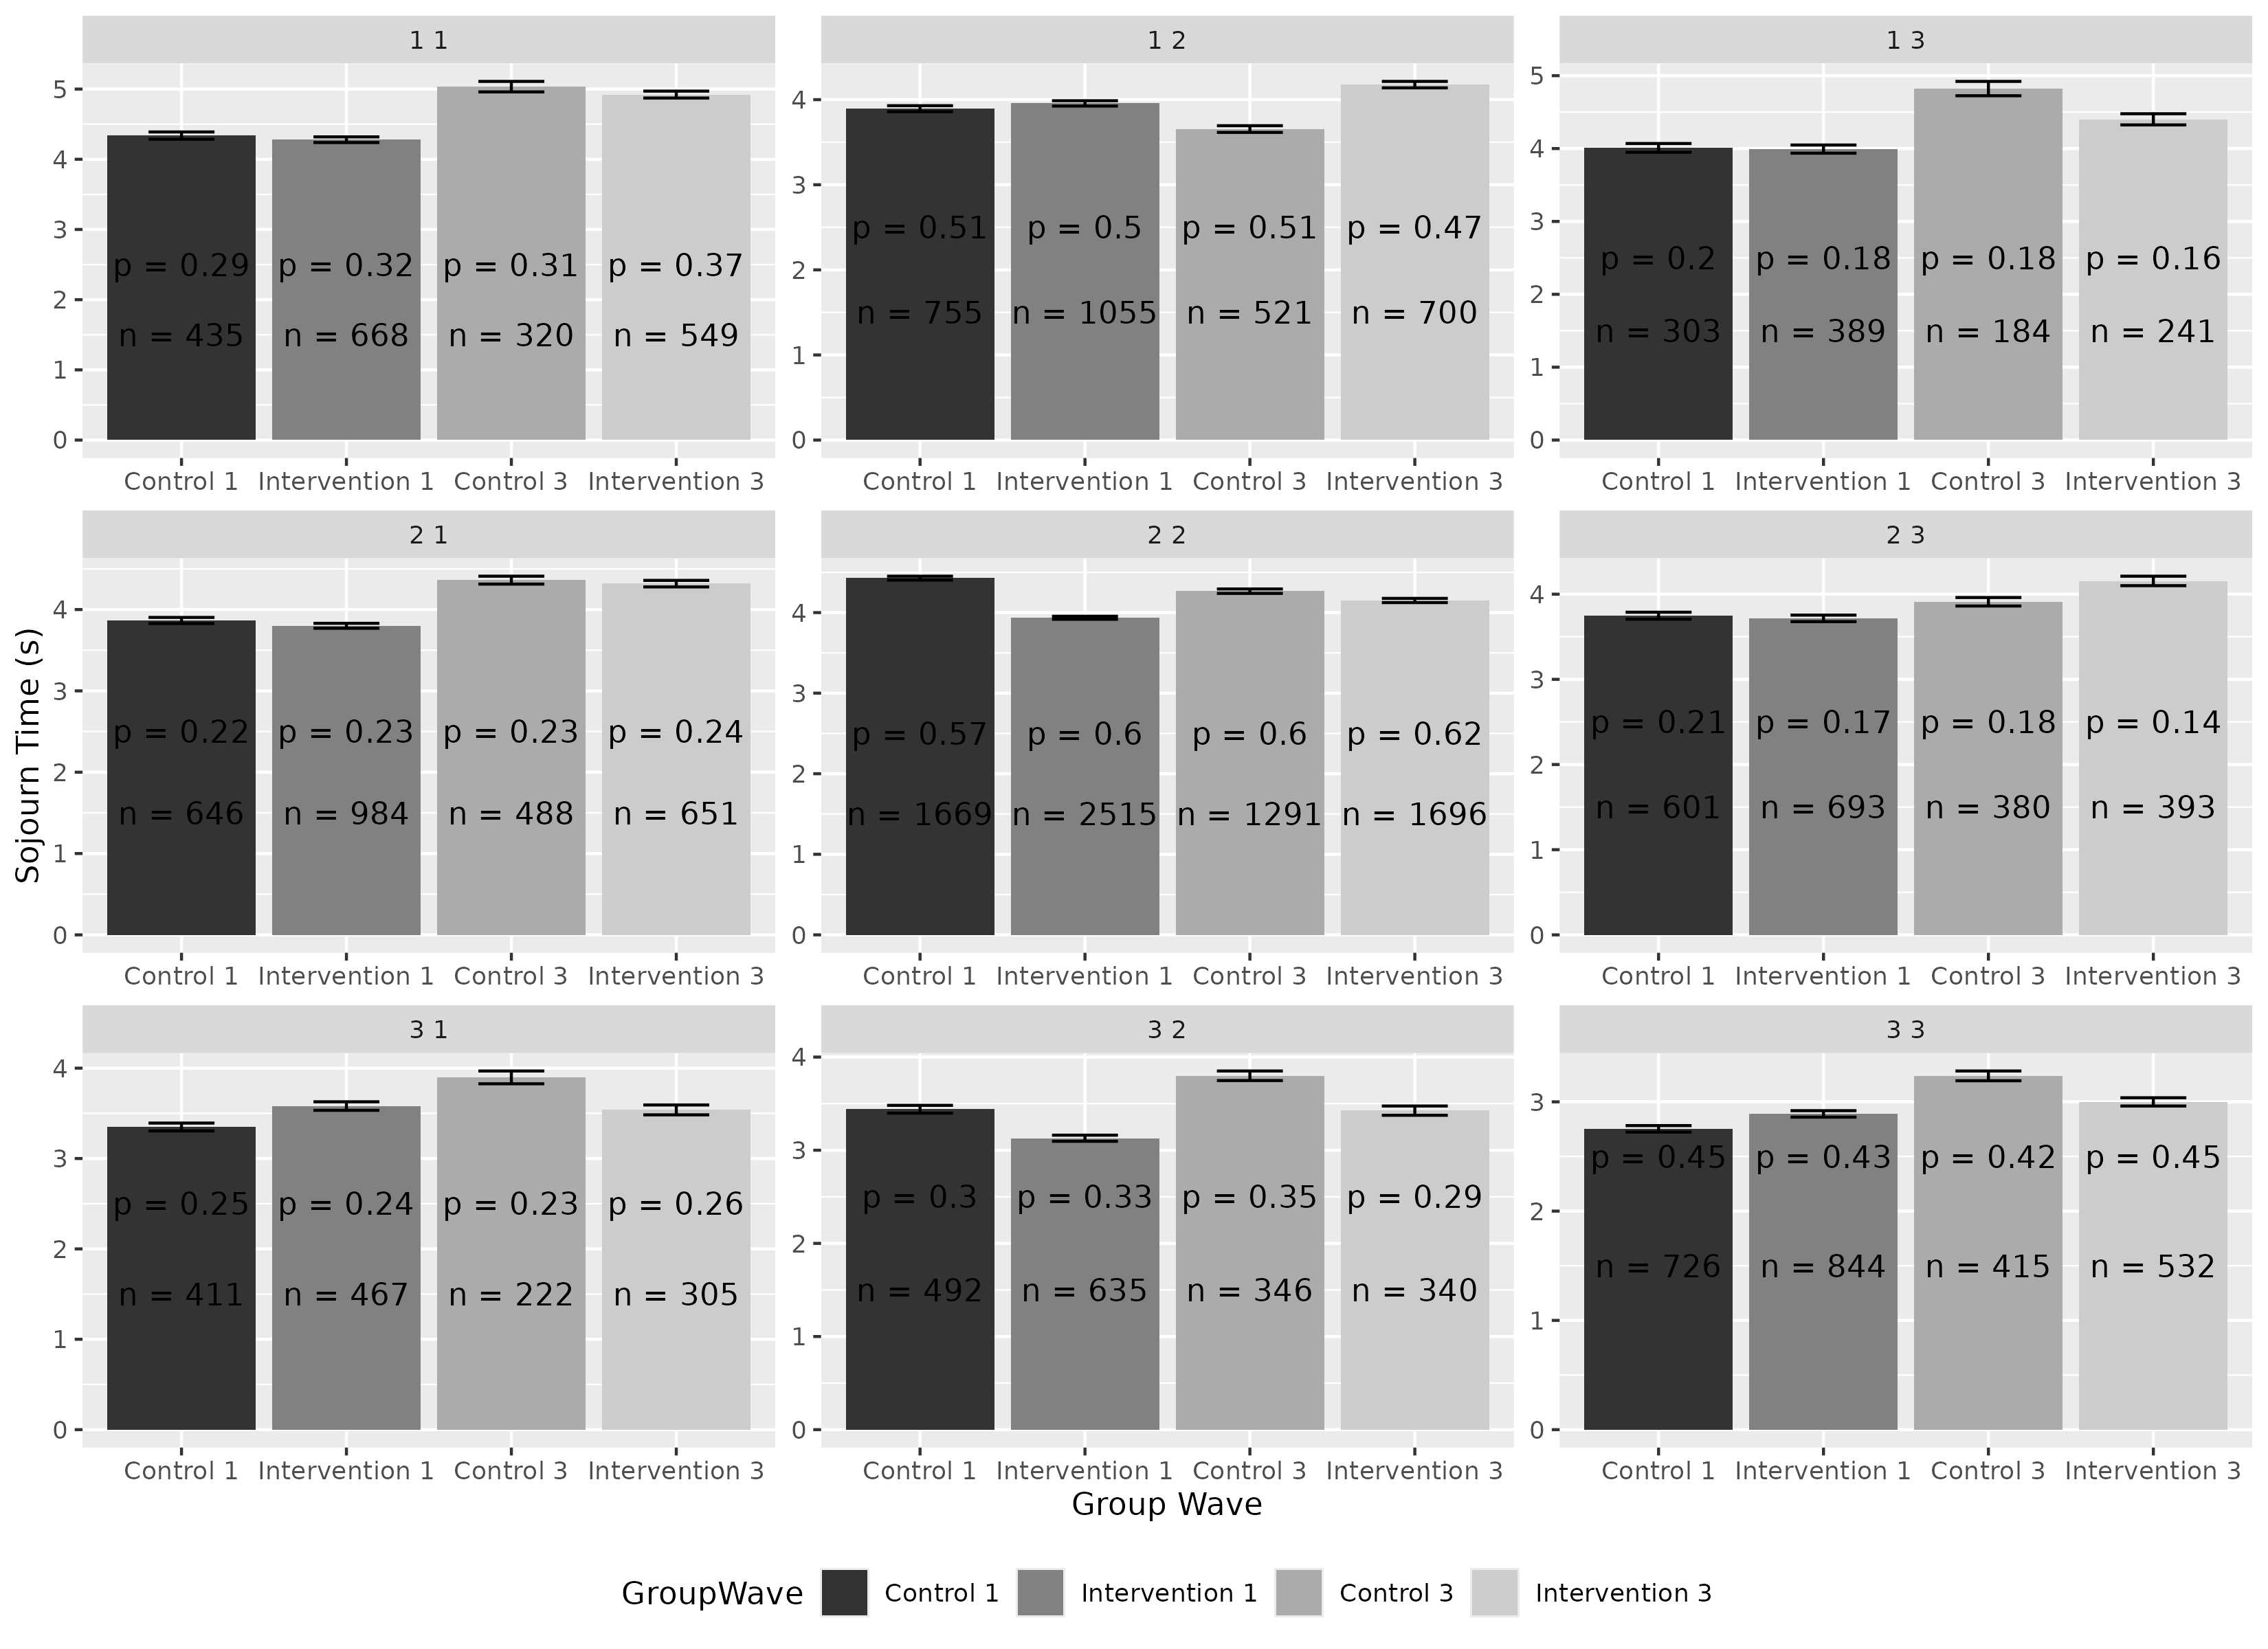
\includegraphics[width=15cm]{figures/generalSojournTimes.png}
\caption{Comparing pre- and post-intervention sojourn times across
groups}
\end{figure}

The next set of analyses examines hazard rates between any of these
transitions. While the previous models examine temporal differences,
these analyses also incorporate the probability of transitions observed
between specific states. The specific transition of interest were
comparing the hazards of transition from PRIDE into PRIDE, comparing the
group by wave interaction. Comparing the hazards of this transition
across groups at the first assessment of the DPICS displays no group
differences (see figure 3.3); however, the post assessment displays a
clear separation in the hazards when comparing the intervention versus
the control group. As the number of PRIDE expressions was greater for
the intervention cohort on the second administration of the DPICs this
growth was predominantly driven by within PRIDE transitions.

\begin{figure}
\centering
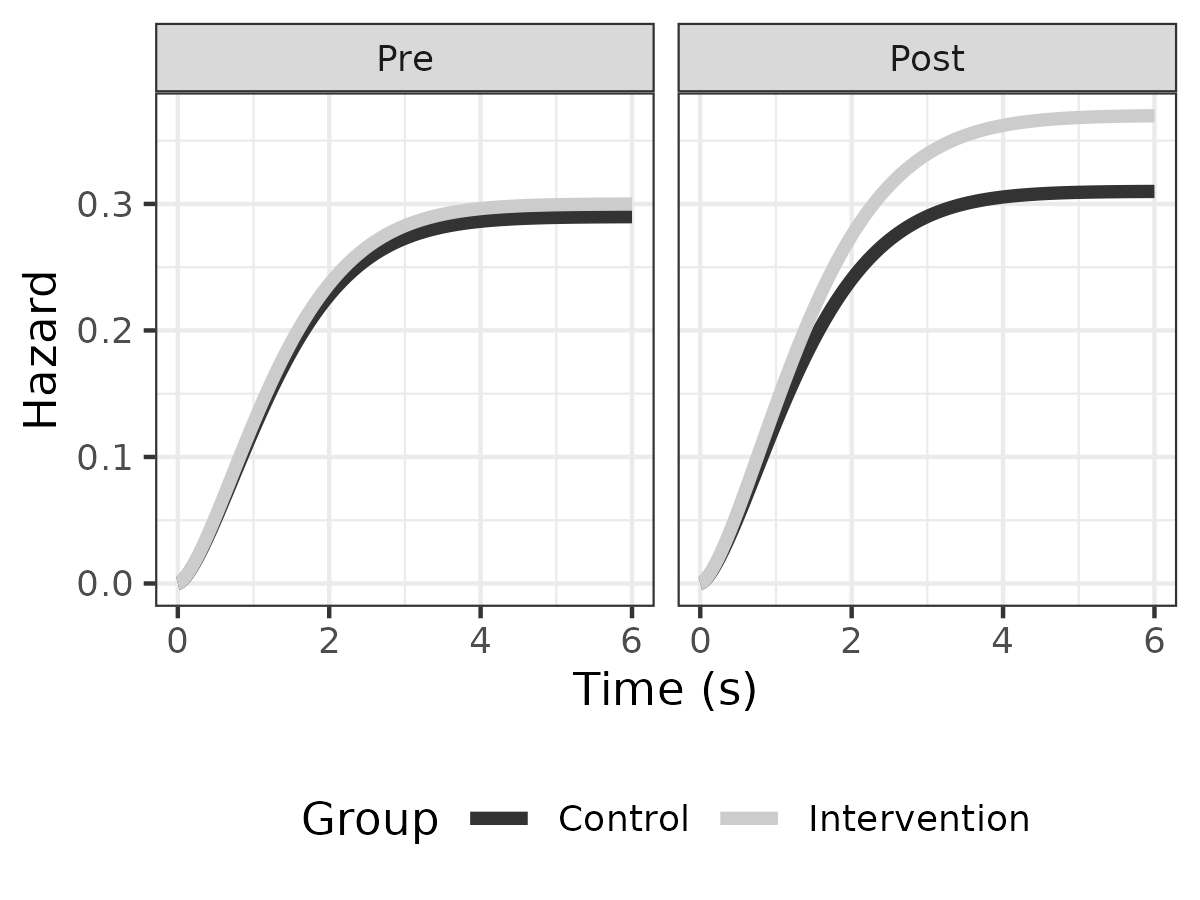
\includegraphics[width=12cm]{figures/allTransOnetoOne.png}
\caption{Comparison for PRIDE to PRIDE hazard rates comparing group and
wave effects}
\end{figure}

\subsection{Examining The Influence of Compliance on The Dynamics Parental Verbal Actions}
The final set of analyses focus specifically on how child compliance
influences the dynamics of parental verbal interactions. A total of 3641
compliable commands were delivered across all groups and waves. Of
these, the majority were complied with (n=2494). In order to examine
these trajectories, child compliance was coded following any compliable
command. The first set of analyses examine the sojourn times for state
transitions following any compliable command delivered by the parent,
which is coded as a PRIDE action by the DPICs (see figure 3.4). The first
effect of interest was the main effect of compliance which increased
sojourn times across all transition types
(\(\beta=0.29, BCI_{lower}=0.01, BCI_{upper}=0.55\)). The second effect
worth highlighting was an interaction involving transition type, group,
and wave, this was observed for the PRIDE into PRIDE transitions. This
interaction suggested a longer sojourn time for the intervention cohort
following a noncompliance compared to the control cohort at second DPICs
assessment(\(\beta=0.48, BCI_{lower}=0.05, BCI_{upper}=0.91\); see
figure 3.4). The last interaction in this same category to highlight
involved transitions from PRIDE into DON'T when comparing case and
control cohorts at second administration of the DPICs. The intervention
cohort saw a increase in their sojourn times when transition from PRIDE
into DON'T on the readministraion of the DPICs
(\(\beta=0.71, BCI_{lower}=0.18, BCI_{upper}=0.1.06\)).

\begin{figure}
\centering
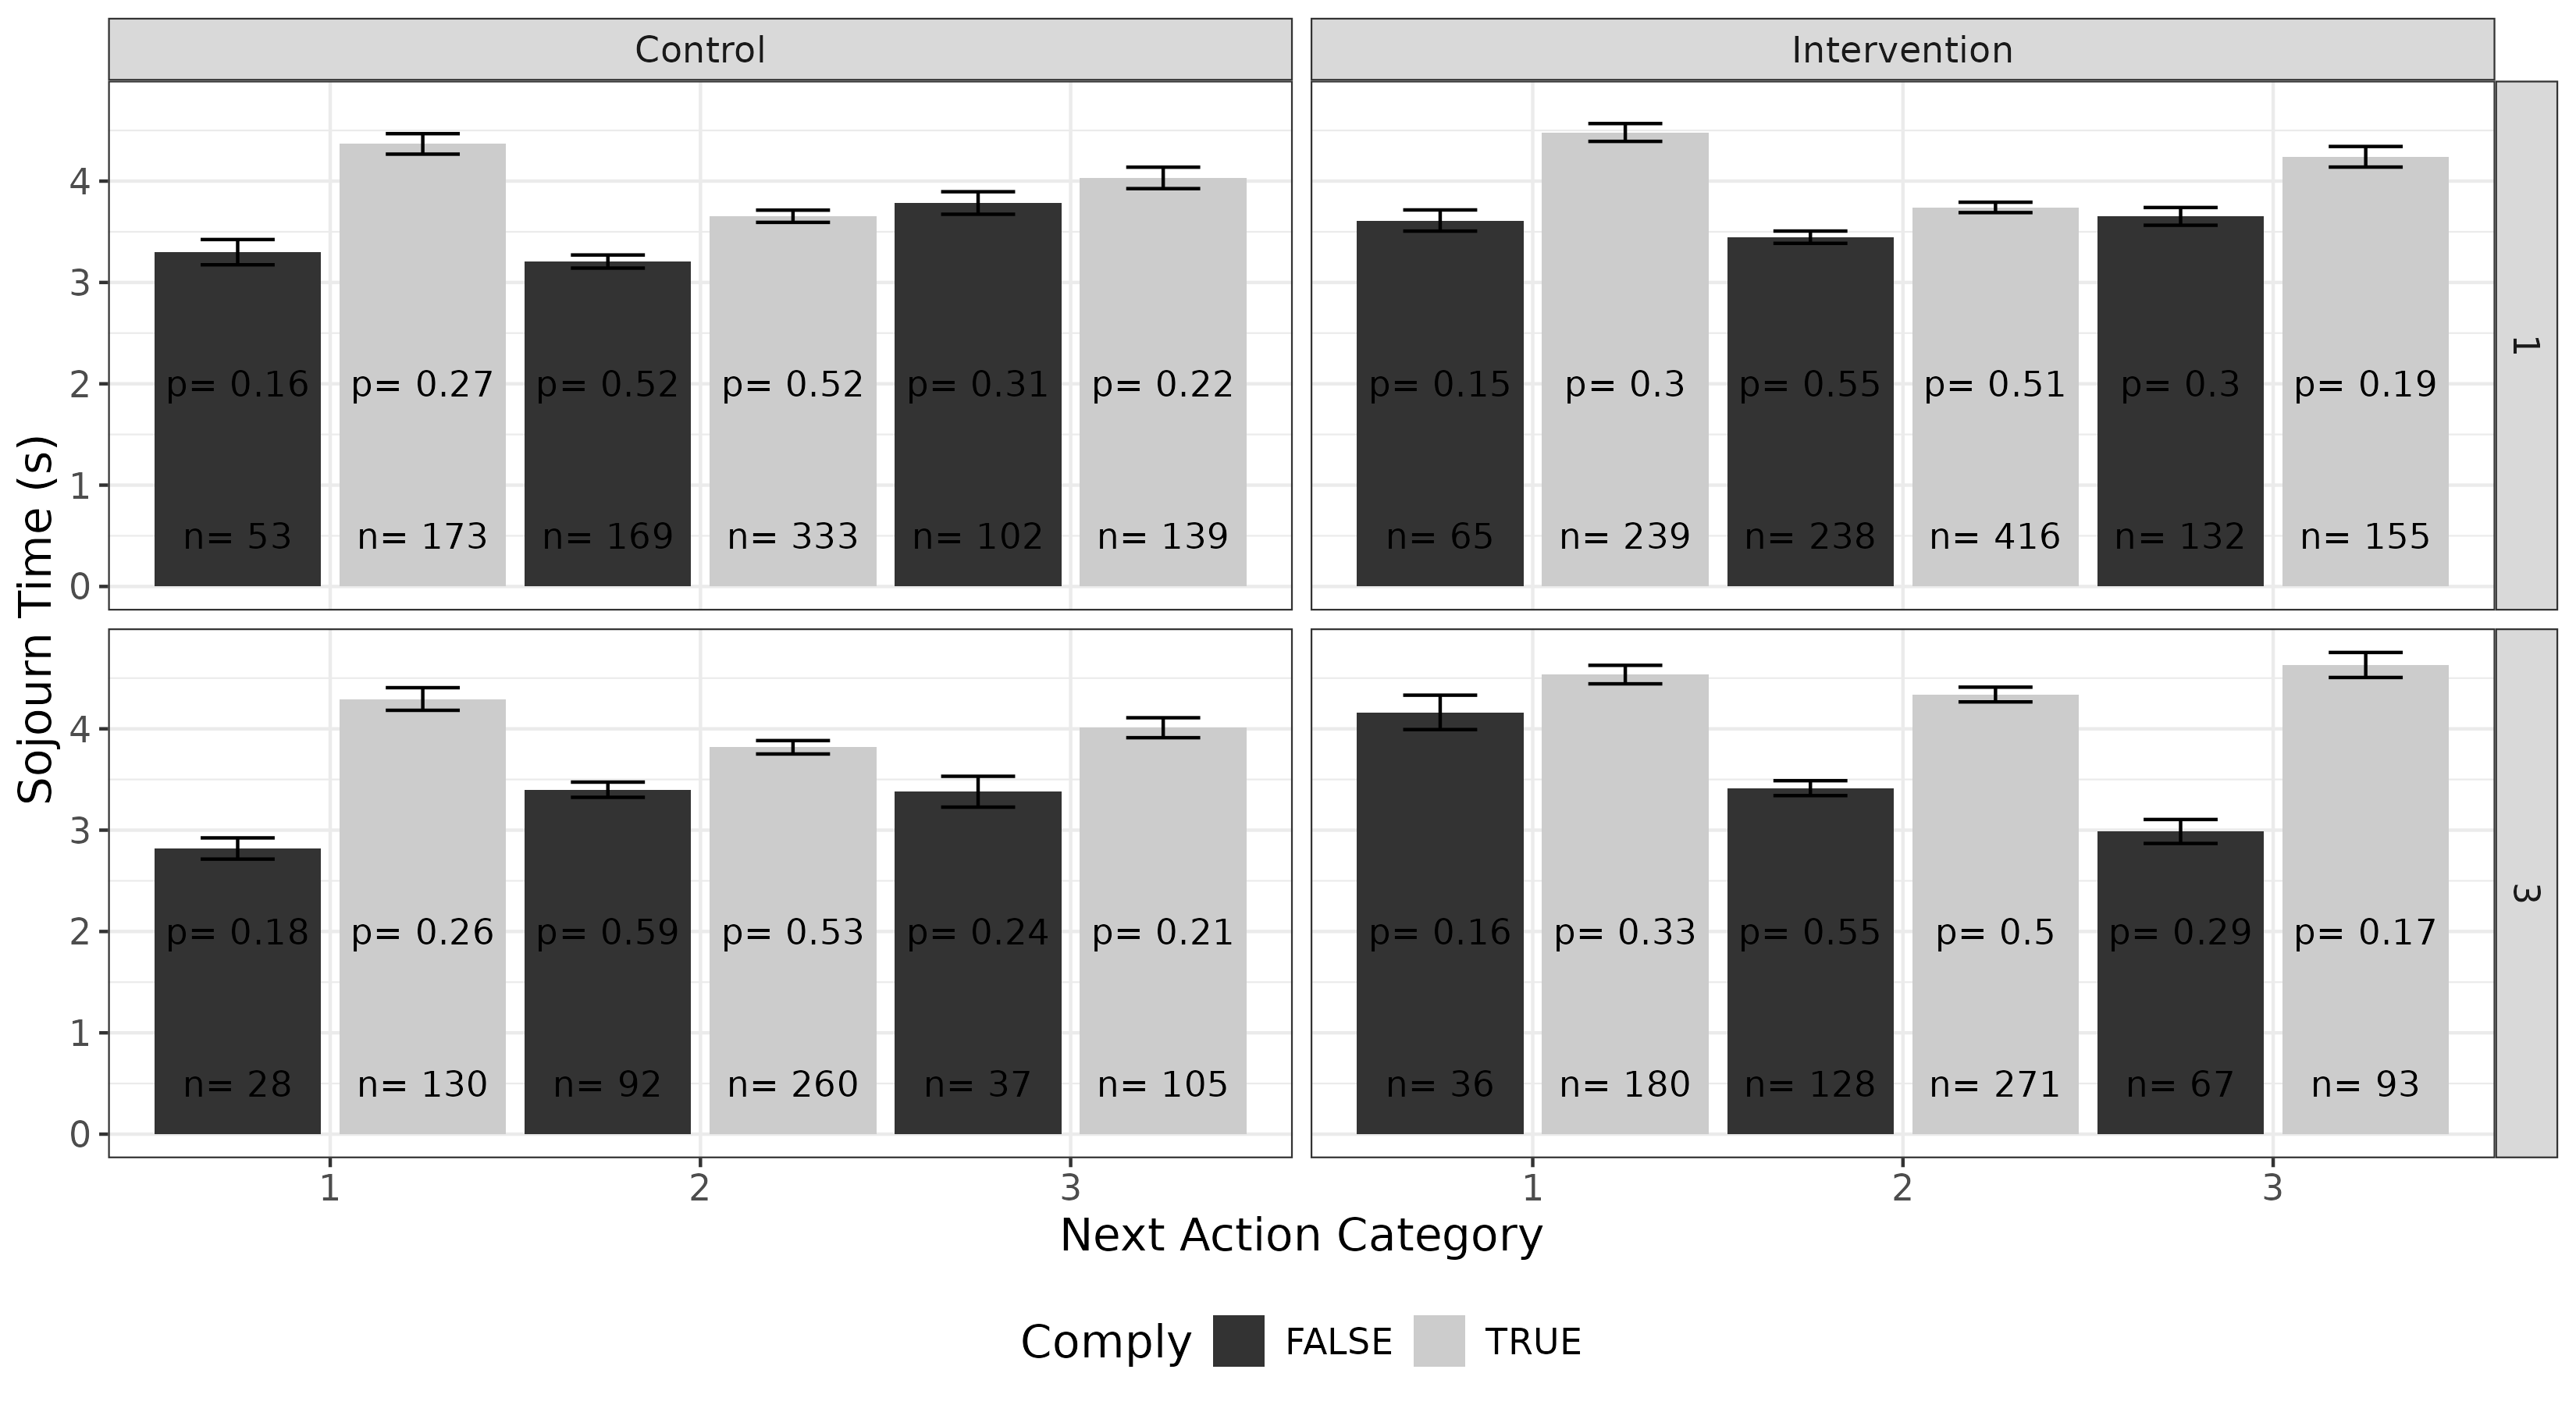
\includegraphics[width=15cm]{figures/complySojournTimes.png}
\caption{Influence of child compliance on sojourn times}
\end{figure}

Finally, the last set of results examines hazards for transitions into
PRIDE across the compliance of the child, wave, and group (see figure
3.5). Hazards at the first administration of the DPICs suggest very
little separation between the groups within a the compliance categories.
A separation is distinguished when comparing the hazards from the second
administration of the DPICs. When a child does not comply to a command,
the control cohort has a higher hazard rate, when a child does comply,
the intervention cohort has a higher hazard.

\begin{figure}
\centering
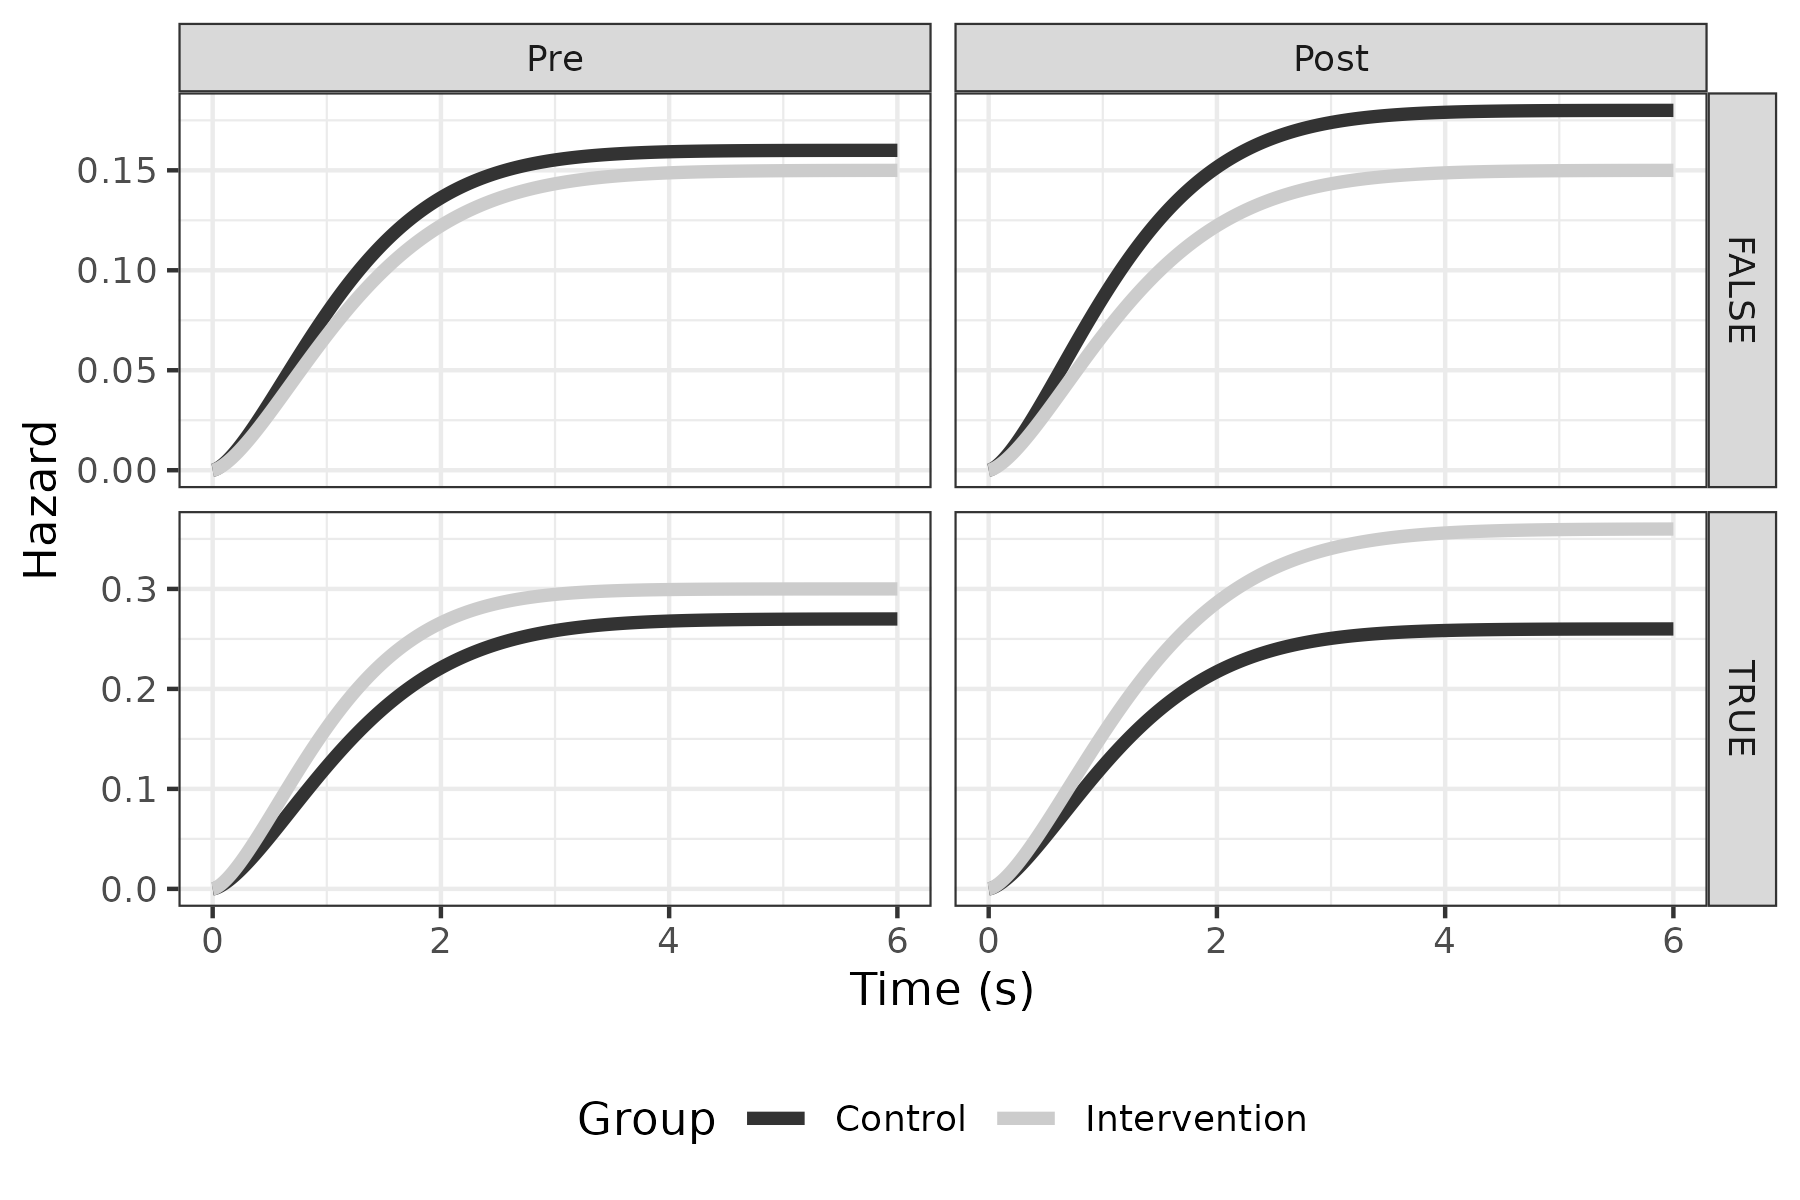
\includegraphics{figures/complyHazOnetoOne.png}
\caption{Hazards comparing PRIDE to PRIDE transitions across group,
wave, and child compliance}
\end{figure}

\newpage

\section{Discussion}
The goal of these analyses was to examine what influence PCIT had on
dyadic verbal interactions during a structured clean-up task as
administered within the DPICs task. This was performed using a
semi-Markov model as parameterized through a multilevel time-to-event
Weibull model. These models examined general dynamics of parental verbal
expressions as well as the influence that a child's compliance has on
their parents. The results displayed both inter- and intra-state
differences and timing when comparing the first and second
administration DPICs, as well as some group differences following the
administration of PCIT.

The largest differences in group dynamics were observed in arguably the
most desirable state in the DPICs hierarchy. Parents in the intervention
cohort displayed greater hazards for a PRIDE into PRIDE transition. As
the goal of PCIT is to encourage clear and concise direction and
positive reward when these actions are performed (Funderburk \& Eyberg,
2011; Lieneman et al., 2017; E. A. Skowron et al., 2024). The PRIDE
state captures the actions that are required to perform this, during the
PCIT sessions parents are instructed to give clear direct commands for
what is being requested of the child, upon completion of the command,
the parent is instructed to praise the child for their compliance. This
is to say the parent is being actively instructed or how to engage in
pride actions and how to maintain in these PRIDE states. This was
evidenced by increased hazards for the PRIDE to PRIDE transitions, as
well as growth in the probability of transitioning from PRIDE into PRIDE
when comparing the control with the intervention cohort.

The second goal of PCIT is lower the frequency of DON'T state
expressions. the DON'T state captures behaviors which are though to be
evoking frustration within the dyad (Schuhmann et al., 1998). For
example, the most frequently expressed DON'T state were noncompliable
command. An example of a noncompliable command would be ``clean up''
where the command is far too ambiguous for the child to comply to these
instructions. The present results offer little differences in the
frequency of these behaviors, for example, the probability of DON'T
intrastate transitions for the control cohort remained relatively stable
(\(p_{d\rightarrow d;t1}=.45;p_{d\rightarrow d;t3}=.42\)), and the
intervention cohort displayed a similar pattern
(\(p_{d\rightarrow d;t1}=.43;p_{d\rightarrow d;t3}=.45\)). One potential
explanation for this was the sample of interest. The current study was
predominantly focused on parent-child dyads who were at high risk of
abuse or neglect. The DON'T actions, and noncompliance are potential
mechanisms for instances of abuse (Rodriguez et al., 2018; Rodriguez \&
Tucker, 2015).

The next set of analyses examines how the compliance from the child
influences the parent's actions. This required a separate model which
was specific to any compliable command the parent expressed. The most
clear separation between the first and second administration of the
DPICs was evidenced in the sojourn times of the PRIDE to PRIDE
transitions. Surprisingly, for the control cohort, when compliance was
not observed their PRIDE exchanges following this noncompliance were
quicker compared to when compliance was observed. Additionally, the
PRIDE following a noncompliance was more than one and a half seconds
quicker in the control cohort (s=2.75) versus the intervention cohort
(s=4.2) following PCIT. Previous research has examined similar patterns
where parent-child dyads reinforced each others negative behaviors
(Lorber et al., 1984). Here a similar pattern is observed, where
noncompliance, when it is followed by a PRIDE behavior, occurs quicker
in the SAU cohort.

Another interesting result from the compliance analyses were how the
sojourn times across all transitions following a compliance were
increased across almost all transitions across group at the second
administration of the DPICs. The exception to this pattern were
transitions into the neutral state for the control cohort (s=3.8). The
main effect of compliance within the intervention cohort may be present
due to the structure of PCIT, where parents are instructed to wait for
their child to complete the task before rewarding the child's behavior.
However, because this main effect exists across both the control and
intervention cohort may be present due to limitations in the DPICs
coding system.

Finally, it is worth noting that the most frequent transitions are
within and between the neutral state. The neutral state may be the least
studied of any of the states, yet it is the state that parents are most
frequently expressing. This pattern is true for both models: parents
displayed a total of 1907 neutral actions following a compliable command
regardless of the child's compliance or not representing more than
half of all possible transitions following a compliable command, and a
total of 12,596 state expressions across the entirety of the clean-up
task, again representing far more than half of all state expressions.

\chapter{Discussion}

As the capabilities of researchers to acquire streams of data from
unique participants increases, the issues of analyzing data acquired
from heterogeneous clusters also increases. Pooling across heterogeneous
populations has been incorporated into many of psychology's
methodological advances. The methods and analyses discussed in this
project showcase the importance and capabilities of multilevel survival
analyses to accommodate heterogeneous populations. The alternatives to
these practices are either case-study, single subject based designs, or
to ignore the nesting and potentially reduce inferential capabilities of
the models. The question now returns to the original methodological
continuum posed by Allport of choosing a location between idiographic and
nomeothetic (Allport, 1937). The methods posed in this analysis seek to
pool information and accommodate within-individual characteristics with population inferential capabilities allowing researchers to straddle the idiographic versus nomeothetic continuum.

The growth of ILD within the psychological sciences demands
methodological development which can accommodate heterogeneous
populations when estimating population fixed effects. Historically, the
motivation from experimental psychological researchers has been to
reduce the impact of individual differences to increase inferential
capabilities of studies (Cronbach, 1957). Now, as methodological
innovation has lead to the introduction of EMA designs, the
experimentalist has less capabilities to control for the individual's
characteristics when designing studies. It now becomes more difficult to
control for population heterogeneity through experimentation in these
open world studies.

Pooling across individuals in ILD studies is not novel. Examples of
multilevel structural equation modeling are present across the
literature. Methods include more basic single unit analysis such as the
auto regressive model, to more advanced state space models such as the
dynamic structural equation modeling (Asparouhov et al., 2018). Examples
exists for multilevel vector autoregressive models (Y. Li et al., 2022), as well as multilevel
factor analysis (Song \& Zhang, 2014). This dissertation describes an
alternative modeling technique which can be applied when data are
manifest-state and continuous-time in nature. Perhaps the motivation in
the psychological sciences is to navigate towards state-space models,
these models are applicable when the true state of the unit of analysis
is better assessed by a measurement or latent model. While the methods
proposed here were described purely using manifest states, the same
multilevel Weibull regression can be used when states are latent (Yu,
2010).

One of the major motivations of this study was to identify how
time-to-event based analyses can be used akin to Markov models. This
alternative framework allows for more flexible parametric distributions
to be used to analyze the hazards of event timing. Additionally, this
parametric approach can accommodate likelihood based estimation
procedures such as maximum likelihood and the Bayesian approaches
utilized in this dissertation. This is important for the advancement of
these analytic approaches given the potential issues when estimating
complex multilevel models in a maximum likelihood approach.

Of course, the utility of these models to researchers is only
feasible once they make their way into software packages which are more
readily accessed. Here in lies the biggest limitation of the methods
examined in this study. There are few software packages which
perform Markov analysis in programming languages such as R. For example
packages such as \texttt{msm} exist, but cannot incorporate a multilevel
modeling framework (Jackson, 2011). To date, there are no software
packages which perform manifest multilevel Markov modeling in
R. One package which can accommodate this workflow within these
analyses is the \texttt{flexsurv} package, which performs time-to-event
analyses, but this is only implemented in a frequentist based approach,
potentially limiting the complexity of random effects. For semi-Markov
models, packages such as \texttt{SemiMarkov} can be used to fit these
models, but multilevel extensions are not included (Król \&
Saint-Pierre, 2015). The software implemented in this package required
Bayesian estimation through the \texttt{STAN} software. Bayesian
software typically has a higher barrier to entry than more commercial
freeware software such as R.

\section{Simulation}

The simulation study examined the capabilities of time-to-event models
to estimate both true Weibull shape parameters and the magnitude of the
population criterion variable. Two parametric distributional families
were used to model simulated sojourn times: exponential and Weibull.
These models were also estimated with and without random effects. A
total of 128 factor permutations were created, 1,000 samples were drawn
within each sample permutation, and four models were estimated within
every sample yielding a total of 512,000 estimated models. The factors
which most heavily influenced the parameter recovery were largely the
magnitude of random variance, and the modeling
strategy used to recover parameters.

Random variance is an ever present issue in psychological data.
Incorporating a multilevel framework across more modeling frameworks
would be prudent for psychologists. The case is further underscored
considering that cognitive questions are theorized to be a random
sampling from all possible questions which can be used to assess a
latent trait (Revelle, 2024; Steyer, 1989; Yarkoni, 2020). The analysis
here were posed in a different manner, that being random samples of
individual's as opposed to questions, but the outcome is the same:
random variance for time-to-event models must be respected. One of the
more pronounced findings was the resilience of the multilevel
exponential and Weibull model to identify the true parameters, as well
as their ability to cover the true population parameter. In fact even
when no random variance was present in the data, the performance of the
multilevel and fixed effect models was near equivalent when examining
criterion variable estimation error. Of course, when random variance was
large, this is when errors were large and nonignorable, on average
the multilevel models displayed error of roughly .77, while the fixed
effect Weibull model displayed an error of .85, and the exponential
model displayed an error larger than 1.2. These results inform
researchers that the most resilient models would be the multilevel
nonconstant hazard (semi-Markov model) with respect to identifying a
criterion variable when random variance may be present in the data.

The second ANOVA examined the capabilities to recover the true shape
parameter. Additionally, an ANCOVA examined error when estimating the criterion
variable's magnitude that can be attributed to the misestimation of the
shape parameter. First, the ability to recover the true shape parameter
was much greater in the multilevel Weibull approach with a mean error of
0.4, compared to the fixed effect approaches mean error of more than
1.4. This is across all simulation factors, but it is important to
incorporate these findings with the ANCOVA results. The ANCOVA provides
a glimpse into how much the criterion variable estimation error can be
attributed to the shape parameter error, roughly 12\% of criterion
variable estimation error can be attributed to the shape parameter
error. This relationship further varied depending upon other sampling
permutations but the results in the best case sampling permutations
still indicated a relatively strong effect. These results suggest the
multilevel Weibull model performed the best at estimating the true shape
parameter, which reduces criterion variable estimation error.

Finally, the logistic regression examined the capabilities for the
estimated models to cover the true parameter within the 95\%-BCI. This
practice follows some best recommendations for the applications of
Bayesian models. The most powerful predictor for recovery was
unsurprisingly sample size. A larger sample size doubled the odds of
correctly recovering the true parameter when ignoring all other sampling
factors. The next best predictors were the application of either a
multilevel exponential or a multilevel Weibull model, with a near
equivalent odds ratio across the both of these. Now, one potential
contributor to this would be the larger ``standard error''; in the
Bayesian instance, this would be the sampling distribution. The
influence of these practices were attempted to be controlled for by only
allowing non-zero BCI intervals for the non-zero criterion variable. That is, both power, the ability to detect an effect, and specificity, the ability to identify a null effect, were examined. 
Additionally, a fairly aggressive sampling practice was taken to reduce
the influence of autocorrelation samples, but the ACF were not examined
due to the number of models estimated.

Across all of these different models, it was surprising how little
influence the additional simulation factors influenced the estimation of
both the criterion and shape error. The additional factors included
observation length, transition matrix, and the range of the scale
parameters. These factors displayed no effect sizes that merited
further discussion. This may either speak to the resilience of the
time-to-event models to recover the true parameters across these
simulation factors, or a potential limitation to how the simulation was
implemented. Regardless, it is worth pointing out that these simulation
factors carried little weight across these models.

Limitations of the simulation study include, but are not limited to, the
methods used to generate the data, the small number of factors included,
the naive priors, and the lack of any estimation error in the criterion
variable. The general take away from the simulation study should
underscore the flexibility of a Bayesian approach using the Weibull
model as an alternative to Markov models for psychologists. However,
because the data were generated by sampling sojourn times from various
Weibull distributions, it should be less surprising that the Weibull
models were the best performing analytic choice. However, the
performance of the Weibull model was near equivalent when the data were
generated from an exponential distribution, which is the distribution
that a continuous-time Markov model employs when estimating transition
intensities (Jackson, 2011; Smith \& Stoneley, 1997). Both the factors,
and their levels, were selected based on a brief literature search of
the application of Markov models across the psychological field, and
specific to the empirical study included in this dissertation. One of
the difficulties for implementing an EMA study is of course, the benefit
of doing so, participants maintain their naturalist lifestyle. This
introduces all possible type of confounding influences that cannot be
controlled. While the simulation protects against any possible sources
of variation that cannot be identified, this of course is not reflective
for the true acquisition of ILD discrete-state data. The selection of
priors in the Bayesian framework is very influential, even more so as
the sample size decreases. Here, diffuse and naive priors were employed
as to ease the implementation and keep a uniform processing stream
across all models, nonetheless, applied scientists should be cautioned to
identify and justify the priors whenever possible. Finally, one of the
biggest and most consistent issues when working with behavioral data is
the reliability and the validity of the data being measured. This
simulation study chose to ignore both of the issues when creating the
the criterion variable. The capabilities of these models to identify the
true relationships were best case scenarios, introducing measurement
error into this equation will likely reduce the models capabilities to
identity these relationships.

The conclusions of this simulation, while considering these limitations,
still suggests the Weibull model in-lieu of the exponential Markov based
approach as an attractive alternative.

\section{Verbal Dynamics of Parents During a Clean-up Task}

The semi-Markov model employed in the empirical study, parameterized as
a time-to-event Weibull regression, sought to examine how parents verbal
behaviors are influenced by both the administration of PCIT, and
compliance from their child. The results suggest that after the administration of PCIT parent's
display greater hazards (i.e.~more likely) to exhibit PRIDE behaviors.
One surprising finding was examined by the timing of PRIDE events
following a noncompliance from the control cohort, where PRIDE behaviors
occurred quicker in time compared to the behaviors where a compliance
was observed.

This study does provide information into how and when PRIDE actions are
likely to occur, this is even more important considering the sample was
composed of families that were at higher risk for abuse and neglect.
This was evidenced by the higher than average adverse childhood experience counts observed in
both the children and their parents. Encouraging positive interactions in
families at a higher risk of externalizing problems has previously been
shown to be a protective factor to reduce externalizing problems in
their children (Deater-Deckard et al., 2004). While the sample here is
not specifically at risk of externalizing behaviors, here we show how
PCIT does move the bar towards greater PRIDE behaviors, and how child's
compliance is greater rewarded with PRIDE behaviors following the
child's compliance in the PICT cohort. These positive interactions are
an important index for the efficacy of intervention (Granic et al.,
2007).

Applying a multilevel semi-Markov model was a novel tool for the
analysis of the DPICS data, and prudent given the magnitude of both the
random variance and the shape parameter. Population dynamics are
unsurprisingly heterogeneous when examining the verbal interactions. The
magnitude of the random variance term was 0.60, suggesting large
heterogeneity in time-to-event patterns across dyads. Additionally, the
estimated shape parameter was 1.5, indicating a monotonically increasing
hazard rate, suggesting a continuous-time Markov model may not be appropriate. The simulation study suggested that when random variance
was large, and the shape parameter was misestimated,
criterion variable error was larger. Thus, the most appropriate
analytic choice for these data was the multilevel semi-Markov model.

The methods applied within this empirical study were utilizing the
minimally coded DPICs data, other studies have expanded the coding
system to better incorporate parent and child behavior into the
analyses. A good example expanding the coding system is observed by
Lunkenheimer et al., where parental behaviors were coded into one of
nine possible behaviors, and the child's were coded into one of seven
possible behaviors. These behaviors were coded as either present or not
present, and were coded on a second-by-second basis. A hidden Markov
model was used to examine the dynamics across nine states composed of
both the child and mothers behaviors. Similar findings were present
suggesting that intra-state transitions of positive, neutral, or DON'T
action transitions were greater (Lunkenheimer et al., 2017).

One realm that has not received much attention in the DPICs analyses is
the most frequently visited state observed in this empirical study. The
most frequent state was the neutral state. This state is composed of
both neutral talk, and questions. The greatest intra-state transition probabilities were in the
neutral state,additionally, the greatest inter-state emissions from PRIDE were into
Neutral, and the same was observed for the DON'T behaviors. The neutral
state composed more than half of all verbal interactions between the
parent and their children, yet, the literature is fairly agnostic to
coding these behaviors, or encouraging them throughout the
administration of the DPICs.

Limitations to the current methods stem both from the coding system
applied as well as the inability to predict the probability of compliance.
Addressing child compliance is an important goal when trying to reduce
externalizing behavior as well as abuse in children (Lind et al., 2020;
Somers et al., 2024). One of the benefits of the clean-up task is also
an inherent drawback, the task is free form in nature. The parents
instruct their children to clean the room, the dyads receive no
further instructions. The verbal interactions are then thought to be as
naturalistic as possible, even though the dyads are being monitored
during the task. The goal of the DPICs is to assess the compliance rates
of children during the clean-up task, but compliance is defined as
compliance to a verbal command from a parent. Some dyads may be
penalized if the child cleans the toys without verbal instruction based
on this coding framework. Thus, a child who completes the task without
verbal instruction, may be summarized as a noncomplient child. Of
course, this is built on an even larger issue inherent to the
discretization of any verbal interaction, the coding systems employed.
The PRIDE behaviors are composed of what are deemed and coached to be
positive interactions by the PCIT therapy, yet the quality of these
PRIDE behaviors is lost based on the binary coding structure employed.
Both direct and indirect commands were included in PRIDE events for this
study when direct commands elicit better compliance. Additionally,
nonverbal actions are ignored completely from these analyses, so any
nonverbal interaction is excluded. This can give the effect that some less verbal dyads
contribute less, when their interactions may be equivalent to any of the
three coded states. Finally, the methodology employed in this study
examines the most probable state transitions, and the timing of these
transitions; however, longer sequences of behaviors may very well
influence these trajectory. For example, PCIT attempts to encourage PRIDE behaviors following compliance, yet these analyses provide little to no insight into the correct sequence of behaviors. Incorporating previous steps can be readily
incorporated into the Weibull regression framework, this process was not
examined in the current study. It would be interesting to better examine
a longer sequence of parental actions and the influence this has on the
child's compliance as well as the dynamics of the parents actions.

\section{Future Work}
The use of time-to-event models are important for questions which answer
``whether or when''; multi-state time-to-event models can be used to
examine similar questions when there are multiple events of interest.
The methodology proposed in this dissertation, that of a multilevel
Weibull regression, should be attractive to psychologists as
continuous-time discrete-state data become more readily available.
Several facets of time-to-events models were not explored in these
analyses such as using censored data. The censoring of data occurs when
the timing of an event is not known. Two types of censoring exist: left
and right censoring, left censoring occurs when the event occurred
within a range of known times, and right censoring occurs when the event
has not yet been observed (Clark et al., 2003). Both of these are
possible to exist in psychological data. Given that typical EMA studies
may not catch the true timing of potential transitions given the
temporally random sampling, incorporating these limitations would be
important for future studies.

Another big appeal for these time-to-event models are the ability to
incorporate both time variant and time-invariant predictors (Lougheed et
al., 2019). Incorporating time variant predictors into longitudinal data
can introduce issues such as non linearity. The empirical analyses in
this study used time variant predictors such as compliance to a command
from a child to their parent. This is a binary predictor in nature, but
data with more complex compositions can be incorporated and
relationships can be modeled using complex approaches such as spline
models.

Finally, stepping back and examining the application of time-to-event
models, psychology can incorporate these models into additional fields
of study. Psychometrics may benefit from these types of models.
Reliability analysis, in the engineering framework, estimates the time
until a system fails. Reliability analysis in the psychometric
literature examines how consistent a test is after repeated
administration. Yet, in the psychological literature, temporal
differences between the readministration of tests are handled in
nonunifrom methods. In fact, the practice effect are typically handled in nonuniform ways generally using techniques that are not appropriate for temporal differences, these practice effects are
very influential across psychological tests (Bartels et al., 2010). The
time-to-event models can be used to examine when scores differ, can
incorporate explanatory variables into predicting these differences, and
of course examine the temporal component of these differences as well.

\section{Conclusion}
Science progresses in incremental steps, having the right data and the
right model facilitates this process. Selecting the best methodology for
time-series analysis further complicates these problems, especially when
data are sampled from a heterogeneous population, or working with dyads
(Gates \& Liu, 2016). The methodology here seeks to address a specific
methodological need when data are composed of nonoverlapping
discrete-state data acquired from a continuous-time sampling procedure.
The Weibull regression offers an attractive methodological stream which
can incorporate complex random effect structures estimated by Bayesian
sampling procedures. An additional distinguishing aspect of the data
examined within these analyses were the presence of both variant and
invariant predictors. The Weibull regression was capable of handling
both, further underscoring why this is an attractive methodological tool
for dyadic analyses.

Using this methodology it was shown how PCIT influences parental
behaviors. Specifically, greater intra-state transitions within the
PRIDE behaviors, as well as PRIDE behaviors following a complied
behavior. These analyses were capable of pulling information across a
wide range of heterogeneous verbal interactions patterns. Other attempts
to perform this have applied multilevel discrete-time Markov models.
This dissertation has showcased the capabilities to pool heterogeneous
continuous-time discrete-state analyses for verbal interactions within
the DPICs protocol. This will facilitate the analysis of similar data,
and can be easily extended to work with multivariate data in a similar
capacity.

\newpage
%
%\nocite{*} % Use to exclude specific citations from *.bib file
\chapter{References}
\bibliographystyle{apa}
\leavevmode\vadjust pre{\hypertarget{ref-abrahamseTreatingChildDisruptive2016}{}}%
Abrahamse, M. E., Junger, M., van Wouwe, M. A. M. M., Boer, F., \&
Lindauer, R. J. L. (2016). Treating {Child Disruptive Behavior} in
{High-Risk Families}: {A Comparative Effectiveness Trial} from a
{Community-Based Implementation}. \emph{Journal of Child and Family
Studies}, \emph{25}(5), 1605--1622.
\url{https://doi.org/10.1007/s10826-015-0322-4}

\leavevmode\vadjust pre{\hypertarget{ref-ainsworthPatternsAttachmentPsychological1978}{}}%
Ainsworth, M. D. S., Blehar, M. C., Waters, E., \& Wall, S. (1978).
\emph{Patterns of attachment: {A} psychological study of the strange
situation} (pp. xviii, 391). Lawrence Erlbaum.

\leavevmode\vadjust pre{\hypertarget{ref-allisonEventHistorySurvival2014}{}}%
Allison, P. D. (2014). \emph{Event {History} and {Survival Analysis}:
{Regression} for {Longitudinal Event Data}}. SAGE Publications.

\leavevmode\vadjust pre{\hypertarget{ref-allportPersonalityPsychologicalInterpretation1937}{}}%
Allport, G. (1937). \emph{Personality {A Psychological Interpretation}}.

\leavevmode\vadjust pre{\hypertarget{ref-altmanMixedHiddenMarkov2007}{}}%
Altman, R. M. (2007). Mixed {Hidden Markov Models}: {An Extension} of
the {Hidden Markov Model} to the {Longitudinal Data Setting}.
\emph{Journal of the American Statistical Association}, \emph{102}(477),
201--210. \url{https://doi.org/10.1198/016214506000001086}

\leavevmode\vadjust pre{\hypertarget{ref-asanjaraniEstimationSemiMarkovMultistate2022}{}}%
Asanjarani, A., Liquet, B., \& Nazarathy, Y. (2022). Estimation of
semi-{Markov} multi-state models: A comparison of the sojourn times and
transition intensities approaches. \emph{The International Journal of
Biostatistics}, \emph{18}(1), 243--262.
\url{https://doi.org/10.1515/ijb-2020-0083}

\leavevmode\vadjust pre{\hypertarget{ref-asparouhovDynamicStructuralEquation2018}{}}%
Asparouhov, T., Hamaker, E. L., \& Muthén, B. (2018). Dynamic
{Structural Equation Models}. \emph{Structural Equation Modeling: A
Multidisciplinary Journal}, \emph{25}(3), 359--388.
\url{https://doi.org/10.1080/10705511.2017.1406803}

\leavevmode\vadjust pre{\hypertarget{ref-austinReviewUseTime2020}{}}%
Austin, P. C., Latouche, A., \& Fine, J. P. (2020). A review of the use
of time-varying covariates in the {Fine}-{Gray} subdistribution hazard
competing risk regression model. \emph{Statistics in Medicine},
\emph{39}(2), 103--113. \url{https://doi.org/10.1002/sim.8399}

\leavevmode\vadjust pre{\hypertarget{ref-balanTutorialFrailtyModels2020}{}}%
Balan, T. A., \& Putter, H. (2020). A tutorial on frailty models.
\emph{Statistical Methods in Medical Research}, \emph{29}(11),
3424--3454. \url{https://doi.org/10.1177/0962280220921889}

\leavevmode\vadjust pre{\hypertarget{ref-bartelsPracticeEffectsHealthy2010}{}}%
Bartels, C., Wegrzyn, M., Wiedl, A., Ackermann, V., \& Ehrenreich, H.
(2010). Practice effects in healthy adults: {A} longitudinal study on
frequent repetitive cognitive testing. \emph{BMC Neuroscience},
\emph{11}(1), 1--12. \url{https://doi.org/10.1186/1471-2202-11-118}

\leavevmode\vadjust pre{\hypertarget{ref-basharinLifeWorkMarkov2004}{}}%
Basharin, G. P., Langville, A. N., \& Naumov, V. A. (2004). The life and
work of {A}.{A}. {Markov}. \emph{Linear Algebra and Its Applications},
\emph{386}, 3--26. \url{https://doi.org/10.1016/j.laa.2003.12.041}

\leavevmode\vadjust pre{\hypertarget{ref-bjorsethEffectivenessParentChildInteraction2016}{}}%
Bjørseth, Å., \& Wichstrøm, L. (2016). Effectiveness of {Parent-Child
Interaction Therapy} ({PCIT}) in the {Treatment} of {Young Children}'s
{Behavior Problems}. {A Randomized Controlled Study}. \emph{PLOS ONE},
\emph{11}(9), e0159845.
\url{https://doi.org/10.1371/journal.pone.0159845}

\leavevmode\vadjust pre{\hypertarget{ref-boydIntroductionMarkovModeling1998}{}}%
Boyd, M. A., \& Lau, S. (1998). \emph{An {Introduction} to {Markov
Modeling}: {Concepts} and {Uses}}.

\leavevmode\vadjust pre{\hypertarget{ref-brainerdMarkovianInterpretationsConservation1979}{}}%
Brainerd, C. J. (1979). Markovian interpretations of conservation
learning. \emph{Psychological Review}, \emph{86}(3), 181--213.
\url{https://doi.org/10.1037/0033-295X.86.3.181}

\leavevmode\vadjust pre{\hypertarget{ref-brykHierarchicalLinearModels1992}{}}%
Bryk, A. S., \& Raudenbush, S. W. (1992). \emph{Hierarchical linear
models: {Applications} and data analysis methods} (pp. xvi, 265). Sage
Publications, Inc.

\leavevmode\vadjust pre{\hypertarget{ref-canasDyadicParentchildInteraction2022a}{}}%
Cañas, M., Ibabe, I., Arruabarrena, I., \& De Paúl, J. (2022). The
dyadic parent-child interaction coding system ({DPICS}): {Negative} talk
as an indicator of dysfunctional mother-child interaction.
\emph{Children and Youth Services Review}, \emph{143}, 106679.
\url{https://doi.org/10.1016/j.childyouth.2022.106679}

\leavevmode\vadjust pre{\hypertarget{ref-canasPromisingObservationalInstruments2020}{}}%
Cañas, M., Ibabe, I., \& De Paúl, J. (2020). Promising observational
instruments of parent-child (0--12 years) interaction within the child
protection system: {A} systematic review. \emph{Child Abuse \& Neglect},
\emph{109}, 104713. \url{https://doi.org/10.1016/j.chiabu.2020.104713}

\leavevmode\vadjust pre{\hypertarget{ref-carrollUseUtilityWeibull2003}{}}%
Carroll, K. J. (2003). On the use and utility of the {Weibull} model in
the analysis of survival data. \emph{Controlled Clinical Trials},
\emph{24}(6), 682--701.
\url{https://doi.org/10.1016/s0197-2456(03)00072-2}

\leavevmode\vadjust pre{\hypertarget{ref-clarkSurvivalAnalysisPart2003}{}}%
Clark, T. G., Bradburn, M. J., Love, S. B., \& Altman, D. G. (2003).
Survival {Analysis Part I}: {Basic} concepts and first analyses.
\emph{British Journal of Cancer}, \emph{89}(2), 232--238.
\url{https://doi.org/10.1038/sj.bjc.6601118}

\leavevmode\vadjust pre{\hypertarget{ref-cooleyParentChildInteraction2014}{}}%
Cooley, M. E., Veldorale-Griffin, A., Petren, R. E., \& Mullis, A. K.
(2014). Parent--{Child Interaction Therapy}: {A Meta-Analysis} of {Child
Behavior Outcomes} and {Parent Stress}. \emph{Journal of Family Social
Work}, \emph{17}(3), 191--208.
\url{https://doi.org/10.1080/10522158.2014.888696}

\leavevmode\vadjust pre{\hypertarget{ref-coxRegressionModelsLifeTables1972}{}}%
Cox, D. R. (1972). Regression {Models} and {Life-Tables}. \emph{Journal
of the Royal Statistical Society. Series B (Methodological)},
\emph{34}(2), 187--220. \url{https://www.jstor.org/stable/2985181}

\leavevmode\vadjust pre{\hypertarget{ref-coxTheoryStochasticProcesses1977}{}}%
Cox, D. R., \& Miller, H. D. (1977). \emph{The {Theory} of {Stochastic
Processes}}. Chapman \& Hall.

\leavevmode\vadjust pre{\hypertarget{ref-cronbachTwoDisciplinesScientific1957}{}}%
Cronbach, L. J. (1957). The two disciplines of scientific psychology.
\emph{American Psychologist}, \emph{12}, 671--684.
\url{https://doi.org/10.1037/h0043943}

\leavevmode\vadjust pre{\hypertarget{ref-dehaan-rietdijkUseMixedMarkov2017}{}}%
de Haan-Rietdijk, S., Kuppens, P., Bergeman, C. S., Sheeber, L. B.,
Allen, N. B., \& Hamaker, E. L. (2017). On the {Use} of {Mixed Markov
Models} for {Intensive Longitudinal Data}. \emph{Multivariate Behavioral
Research}, \emph{52}(6), 747--767.
\url{https://doi.org/10.1080/00273171.2017.1370364}

\leavevmode\vadjust pre{\hypertarget{ref-deater-deckardMotherFatherChildMutuality2004}{}}%
Deater-Deckard, K., Atzaba-Poria, N., \& Pike, A. (2004). Mother- and
{Father-Child Mutuality} in {Anglo} and {Indian British Families}: {A
Link} with {Lower Externalizing Problems}. \emph{Journal of Abnormal
Child Psychology}, \emph{32}(6), 609--620.
\url{https://doi.org/10.1023/B:JACP.0000047210.81880.14}

\leavevmode\vadjust pre{\hypertarget{ref-DefinitionNOMOTHETIC}{}}%
\emph{Definition of {NOMOTHETIC}}. (2024).
https://www.merriam-webster.com.

\leavevmode\vadjust pre{\hypertarget{ref-dellaringaDeterminantsUnemploymentDuration1988}{}}%
Dell'Aringa, C., \& Lodovici, M. S. (1988). Determinants of
{Unemployment Duration} for {Displaced Workers}. \emph{LABOUR},
\emph{2}(3), 91--111.
\url{https://doi.org/10.1111/j.1467-9914.1988.tb00141.x}

\leavevmode\vadjust pre{\hypertarget{ref-elmahdyNewApproachWeibull2015}{}}%
Elmahdy, E. E. (2015). A new approach for {Weibull} modeling for
reliability life data analysis. \emph{Applied Mathematics and
Computation}, \emph{250}, 708--720.
\url{https://doi.org/10.1016/j.amc.2014.10.036}

\leavevmode\vadjust pre{\hypertarget{ref-eybergParentChildInteractionTherapy1988}{}}%
Eyberg, S. (1988). Parent-{Child Interaction Therapy}: {Integration} of
{Traditional} and {Behavioral Concerns}. \emph{Child \& Family Behavior
Therapy}, \emph{10}(1), 33--46.
\url{https://doi.org/10.1300/J019v10n01_04}

\leavevmode\vadjust pre{\hypertarget{ref-eybergDyadicParentChildLnteraction2014}{}}%
Eyberg, S. M., Chase, R. M., Fernandez, M. A., \& Nelson, M. M. (2014).
\emph{Dyadic {Parent-Child} lnteraction {Coding System} ({DPICS-IV})
{Clinical Manual Fourth Edition}.} PCIT International.

\leavevmode\vadjust pre{\hypertarget{ref-eybergConductProblemBehavior1983}{}}%
Eyberg, S. M., \& Robinson, E. A. (1983). Conduct problem behavior:
{Standardization} of a behavioral rating. \emph{Journal of Clinical
Child Psychology}, \emph{12}(3), 347--354.
\url{https://doi.org/10.1080/15374418309533155}

\leavevmode\vadjust pre{\hypertarget{ref-fergusonQuantitativeEstimatesSensory1932}{}}%
Ferguson, A. (1932). Quantitative {Estimates} of {Sensory Events}.
\emph{Nature}, \emph{130}(3291), 810--810.
\url{https://doi.org/10.1038/130810a0}

\leavevmode\vadjust pre{\hypertarget{ref-fichmanAttendanceMakesHeart1989}{}}%
Fichman, M. (1989). Attendance makes the heart grow fonder: {A} hazard
rate approach to modeling attendance. \emph{Journal of Applied
Psychology}, \emph{74}(2), 325--335.
\url{https://doi.org/10.1037/0021-9010.74.2.325}

\leavevmode\vadjust pre{\hypertarget{ref-freudOriginDevelopmentPsychoanalysis1910}{}}%
Freud, S. (1910). The origin and development of psychoanalysis.
\emph{The American Journal of Psychology}, \emph{21}(2), 181--218.
\url{https://doi.org/10.2307/1413001}

\leavevmode\vadjust pre{\hypertarget{ref-funderburkParentChildInteraction2011}{}}%
Funderburk, B. W., \& Eyberg, S. (2011). Parent--child interaction
therapy. In \emph{History of psychotherapy: {Continuity} and change, 2nd
ed} (pp. 415--420). American Psychological Association.
\url{https://doi.org/10.1037/12353-021}

\leavevmode\vadjust pre{\hypertarget{ref-gardnerHierarchicalContinuoustimeSequential1993}{}}%
Gardner, W. (1993). Hierarchical continuous-time sequential analysis:
{A} strategy for clinical research. \emph{Journal of Consulting and
Clinical Psychology}, \emph{61}(6), 975--983.
\url{https://doi.org/10.1037/0022-006X.61.6.975}

\leavevmode\vadjust pre{\hypertarget{ref-gardnerMethodsAnalysisParallel1989}{}}%
Gardner, W., \& Griffin, W. A. (1989). Methods for the analysis of
parallel streams of continuously recorded social behaviors.
\emph{Psychological Bulletin}, \emph{105}(3), 446--455.
\url{https://doi.org/10.1037/0033-2909.105.3.446}

\leavevmode\vadjust pre{\hypertarget{ref-gatesMethodsQuantifyingPatterns2016}{}}%
Gates, K. M., \& Liu, S. (2016). Methods for {Quantifying Patterns} of
{Dynamic Interactions} in {Dyads}. \emph{Assessment}, \emph{23}(4),
459--471. \url{https://doi.org/10.1177/1073191116641508}

\leavevmode\vadjust pre{\hypertarget{ref-gelmanInferenceIterativeSimulation1992}{}}%
Gelman, A., \& Rubin, D. B. (1992). Inference from {Iterative Simulation
Using Multiple Sequences}. \emph{Statistical Science}, \emph{7}(4),
457--472. \url{https://doi.org/10.1214/ss/1177011136}

\leavevmode\vadjust pre{\hypertarget{ref-gmeinwieserRiskPsychotherapyDropout2020}{}}%
Gmeinwieser, S., Schneider, K. S., Bardo, M., Brockmeyer, T., \&
Hagmayer, Y. (2020). Risk for psychotherapy drop-out in survival
analysis: {The} influence of general change mechanisms and symptom
severity. \emph{Journal of Counseling Psychology}, \emph{67}(6),
712--722. \url{https://doi.org/10.1037/cou0000418}

\leavevmode\vadjust pre{\hypertarget{ref-goodmanStatisticalMethodsMoverStayer1961}{}}%
Goodman, L. A. (1961). Statistical {Methods} for the {Mover-Stayer
Model}. \emph{Journal of the American Statistical Association},
\emph{56}(296), 841--868.
\url{https://doi.org/10.1080/01621459.1961.10482130}

\leavevmode\vadjust pre{\hypertarget{ref-granicDynamicSystemsAnalysis2007}{}}%
Granic, I., O'Hara, A., Pepler, D., \& Lewis, M. D. (2007). A {Dynamic
Systems Analysis} of {Parent}--child {Changes Associated} with
{Successful} {``{Real-world}''} {Interventions} for {Aggressive
Children}. \emph{Journal of Abnormal Child Psychology}, \emph{35}(5),
845--857. \url{https://doi.org/10.1007/s10802-007-9133-4}

\leavevmode\vadjust pre{\hypertarget{ref-gridleyComparingLiveVideo2018}{}}%
Gridley, N., Bywater, T. J., \& Hutchings, J. M. (2018). Comparing
{Live} and {Video Observation} to {Assess Early Parent-child
Interactions} in the {Home}. \emph{Journal of Child and Family Studies},
\emph{27}(6), 1818--1829.
\url{https://doi.org/10.1007/s10826-018-1039-y}

\leavevmode\vadjust pre{\hypertarget{ref-hechtContinuoustimeModelingPrevention2021}{}}%
Hecht, M., \& Voelkle, M. C. (2021). Continuous-time modeling in
prevention research: {An} illustration. \emph{International Journal of
Behavioral Development}, \emph{45}(1), 19--27.
\url{https://doi.org/10.1177/0165025419885026}

\leavevmode\vadjust pre{\hypertarget{ref-herzogFirstRecoveryAnorexia1997}{}}%
Herzog, W., Schellberg, D., \& Deter, H.-C. (1997). First recovery in
anorexia nervosa patients in the long-term course: {A} discrete-time
survival analysis. \emph{Journal of Consulting and Clinical Psychology},
\emph{65}(1), 169--177. \url{https://doi.org/10.1037/0022-006X.65.1.169}

\leavevmode\vadjust pre{\hypertarget{ref-homanNoUturnSamplerAdaptively2014}{}}%
Homan, M. D., \& Gelman, A. (2014). The {No-U-turn} sampler: Adaptively
setting path lengths in {Hamiltonian Monte Carlo}. \emph{The Journal of
Machine Learning Research}, \emph{15}(1), 1593--1623.

\leavevmode\vadjust pre{\hypertarget{ref-hougaardFrailtyModelsSurvival1995}{}}%
Hougaard, P. (1995). Frailty models for survival data. \emph{Lifetime
Data Analysis}, \emph{1}(3), 255--273.
\url{https://doi.org/10.1007/BF00985760}

\leavevmode\vadjust pre{\hypertarget{ref-ikbalEstimatingWeibullParameters2022}{}}%
Ikbal, N. A. M., Halim, S. A., \& Ali, N. (Mar-2022). Estimating
{Weibull Parameters Using Maximum Likelihood Estimation} and {Ordinary
Least Squares}: {Simulation Study} and {Application} on {Meteorological
Data}. \emph{Mathematics and Statistics}, \emph{10}(2), 269--292.
\url{https://doi.org/10.13189/ms.2022.100201}

\leavevmode\vadjust pre{\hypertarget{ref-jacksonMultiStateModelsPanel2011}{}}%
Jackson, C. (2011). Multi-{State Models} for {Panel Data}: {The} msm
{Package} for {R}. \emph{Journal of Statistical Software}, \emph{38},
1--28. \url{https://doi.org/10.18637/jss.v038.i08}

\leavevmode\vadjust pre{\hypertarget{ref-kaplanNonparametricEstimationIncomplete1958}{}}%
Kaplan, E. L., \& Meier, P. (1958). Nonparametric {Estimation} from
{Incomplete Observations}. \emph{Journal of the American Statistical
Association}, \emph{53}(282), 457--481.
\url{https://doi.org/10.1080/01621459.1958.10501452}

\leavevmode\vadjust pre{\hypertarget{ref-kayUseAcceleratedFailure2002}{}}%
Kay, R., \& Kinnersley, N. (2002). On the {Use} of the {Accelerated
Failure Time Model As An Alternative} to the {Proportional Hazards
Model} in the {Treatment} of {Time} to {Event Data}: {A Case Study} in
{Influenza}. \emph{Drug Information Journal : DIJ / Drug Information
Association}, \emph{36}(3), 571--579.
\url{https://doi.org/10.1177/009286150203600312}

\leavevmode\vadjust pre{\hypertarget{ref-keileySurvivalAnalysisFamily2005}{}}%
Keiley, M. K., \& Martin, N. C. (2005). Survival {Analysis} in {Family
Research}. \emph{Journal of Family Psychology}, \emph{19}(1), 142--156.
\url{https://doi.org/10.1037/0893-3200.19.1.142}

\leavevmode\vadjust pre{\hypertarget{ref-koenigTransitionsAlcoholUse2020}{}}%
Koenig, L. B., Haber, J. R., \& Jacob, T. (2020). Transitions in alcohol
use over time: A survival analysis. \emph{BMC Psychology}, \emph{8}(1),
115. \url{https://doi.org/10.1186/s40359-020-00479-1}

\leavevmode\vadjust pre{\hypertarget{ref-krolSemiMarkovPackageParametric2015}{}}%
Król, A., \& Saint-Pierre, P. (2015). {SemiMarkov}: {An R Package} for
{Parametric Estimation} in {Multi-State Semi-Markov Models}.
\emph{Journal of Statistical Software}, \emph{66}, 1--16.
\url{https://doi.org/10.18637/jss.v066.i06}

\leavevmode\vadjust pre{\hypertarget{ref-kruschkeBayesianDataAnalysis2018}{}}%
Kruschke, J. K., \& Liddell, T. M. (2018). Bayesian data analysis for
newcomers. \emph{Psychonomic Bulletin \& Review}, \emph{25}(1),
155--177. \url{https://doi.org/10.3758/s13423-017-1272-1}

\leavevmode\vadjust pre{\hypertarget{ref-leeDesistanceSeverityAlcohol2018}{}}%
Lee, M. R., Boness, C. L., McDowell, Y. E., Vergés, A., Steinley, D. L.,
\& Sher, K. J. (2018). Desistance and {Severity} of {Alcohol Use
Disorder}: {A Lifespan-Developmental Investigation}. \emph{Clinical
Psychological Science}, \emph{6}(1), 90--105.
\url{https://doi.org/10.1177/2167702617736852}

\leavevmode\vadjust pre{\hypertarget{ref-le-rademacherUtilityMultistateModels2022}{}}%
Le-Rademacher, J. G., Therneau, T. M., \& Ou, F.-S. (2022). The
{Utility} of {Multistate Models}: {A Flexible Framework} for
{Time-to-Event Data}. \emph{Current Epidemiology Reports}, \emph{9}(3),
183--189. \url{https://doi.org/10.1007/s40471-022-00291-y}

\leavevmode\vadjust pre{\hypertarget{ref-liApplyingMarkovChain2020}{}}%
Li, D., Duys, D., \& Granello, D. (2020). Applying {Markov Chain
Analysis} to {Supervisory Interactions}. \emph{Journal of Counselor
Preparation and Supervision}, \emph{13}(1).
https://doi.org/\url{http://dx.doi.org/10.7729/131.1325}

\leavevmode\vadjust pre{\hypertarget{ref-liFittingMultilevelVector2022}{}}%
Li, Y., Wood, J., Ji, L., Chow, S.-M., \& Oravecz, Z. (2022). Fitting
{Multilevel Vector Autoregressive Models} in {Stan}, {JAGS}, and
{Mplus}. \emph{Structural Equation Modeling: A Multidisciplinary
Journal}, \emph{29}(3), 452--475.
\url{https://doi.org/10.1080/10705511.2021.1911657}

\leavevmode\vadjust pre{\hypertarget{ref-lienemanParentChildInteraction2017}{}}%
Lieneman, C. C., Brabson, L. A., Highlander, A., Wallace, N. M., \&
McNeil, C. B. (2017). Parent--{Child Interaction Therapy}: Current
perspectives. \emph{Psychology Research and Behavior Management},
\emph{10}, 239--256. \url{https://doi.org/10.2147/PRBM.S91200}

\leavevmode\vadjust pre{\hypertarget{ref-limBriefIntroductionParametric2021}{}}%
Lim, H.-S. (2021). Brief introduction to parametric time to event model.
\emph{Translational and Clinical Pharmacology}, \emph{29}(1), 1--5.
\url{https://doi.org/10.12793/tcp.2021.29.e7}

\leavevmode\vadjust pre{\hypertarget{ref-lindPromotingComplianceChildren2020}{}}%
Lind, T., Bernard, K., Yarger, H. A., \& Dozier, M. (2020). Promoting
{Compliance} in {Children Referred} to {Child Protective Services}: {A
Randomized Clinical Trial}. \emph{Child Development}, \emph{91}(2),
563--576. \url{https://doi.org/10.1111/cdev.13207}

\leavevmode\vadjust pre{\hypertarget{ref-lindak.muthenMplusUserGuide2017}{}}%
Linda K., Muthén, \& Bengt O., Muthén. (2017). \emph{Mplus {User}'s
{Guide}}.

\leavevmode\vadjust pre{\hypertarget{ref-lorberSocialLearningApproach1984}{}}%
Lorber, R., Felton, D. K., \& Reid, J. B. (1984). A social learning
approach to the reduction of coercive processes in child abusive
families: {A} molecular analysis. \emph{Advances in Behaviour Research
and Therapy}, \emph{6}(1), 29--45.
\url{https://doi.org/10.1016/0146-6402(84)90011-0}

\leavevmode\vadjust pre{\hypertarget{ref-lougheedMultilevelSurvivalAnalysis2019}{}}%
Lougheed, J. P., Benson, L., Cole, P. M., \& Ram, N. (2019). Multilevel
{Survival Analysis}: {Studying} the {Timing} of {Children}'s {Recurring
Behaviors}. \emph{Developmental Psychology}, \emph{55}(1), 53--65.
\url{https://doi.org/10.1037/dev0000619}

\leavevmode\vadjust pre{\hypertarget{ref-lukeTimeChangeUsing1998}{}}%
Luke, D. A., \& Homan, S. M. (1998). Time and change: {Using} survival
analysis in clinical assessment and treatment evaluation.
\emph{Psychological Assessment}, \emph{10}(4), 360--378.
\url{https://doi.org/10.1037/1040-3590.10.4.360}

\leavevmode\vadjust pre{\hypertarget{ref-lunkenheimerHarshParentingChild2017}{}}%
Lunkenheimer, E., Ram, N., Skowron, E. A., \& Yin, P. (2017). Harsh
parenting, child behavior problems, and the dynamic coupling of parents'
and children's positive behaviors. \emph{Journal of Family Psychology},
\emph{31}(6), 689--698. \url{https://doi.org/10.1037/fam0000310}

\leavevmode\vadjust pre{\hypertarget{ref-markovExampleStatisticalInvestigation1913}{}}%
Markov, A. A. (1913). An example of statistical investigation of the
text {Eugene Onegin} con- cerning the connection of samples in chains.
({In Russian}.). \emph{Bulletin of the Imperial Academy of Sciences of
St. Petersburg}, \emph{7}(3), 153--162.

\leavevmode\vadjust pre{\hypertarget{ref-maruottiMixedNonhomogeneousHidden2012}{}}%
Maruotti, A., \& Rocci, R. (2012). A mixed non-homogeneous hidden
{Markov} model for categorical data, with application to alcohol
consumption. \emph{Statistics in Medicine}, \emph{31}(9), 871--886.
\url{https://doi.org/10.1002/sim.4478}

\leavevmode\vadjust pre{\hypertarget{ref-mcneishPracticalGuideSelecting2023}{}}%
McNeish, D. (2023). A practical guide to selecting and blending
approaches for clustered data: {Clustered} errors, multilevel models,
and fixed-effect models. \emph{Psychological Methods}, No Pagination
Specified--No Pagination Specified.
\url{https://doi.org/10.1037/met0000620}

\leavevmode\vadjust pre{\hypertarget{ref-mcneishModelingIndividualDifferences2021}{}}%
McNeish, D., Bauer, D. J., Dumas, D., Clements, D. H., Cohen, J. R.,
Lin, W., Sarama, J., \& Sheridan, M. A. (2021). Modeling individual
differences in the timing of change onset and offset.
\emph{Psychological Methods}, No Pagination Specified--No Pagination
Specified. \url{https://doi.org/10.1037/met0000407}

\leavevmode\vadjust pre{\hypertarget{ref-meira-machadoMultistateModelsAnalysis2009}{}}%
Meira-Machado, L., de Uña-Álvarez, J., Cadarso-Suárez, C., \& Andersen,
P. K. (2009). Multi-state models for the analysis of time-to-event data.
\emph{Statistical Methods in Medical Research}, \emph{18}(2), 195--222.
\url{https://doi.org/10.1177/0962280208092301}

\leavevmode\vadjust pre{\hypertarget{ref-millerFiniteMarkovProcesses1952}{}}%
Miller, G. A. (1952). Finite markov processes in psychology.
\emph{Psychometrika}, \emph{17}(2), 149--167.
\url{https://doi.org/10.1007/BF02288779}

\leavevmode\vadjust pre{\hypertarget{ref-moritaIntroducingSurvivalAnalysis1989}{}}%
Morita, J. G., Lee, T. W., \& Mowday, R. T. (1989). Introducing survival
analysis to organizational researchers: {A} selected application to
turnover research. \emph{Journal of Applied Psychology}, \emph{74}(2),
280--292. \url{https://doi.org/10.1037/0021-9010.74.2.280}

\leavevmode\vadjust pre{\hypertarget{ref-nekkantiStudyProtocolCoaching2020}{}}%
Nekkanti, A. K., Jeffries, R., Scholtes, C. M., Shimomaeda, L., DeBow,
K., Norman Wells, J., Lyons, E. R., Giuliano, R. J., Gutierrez, F. J.,
\& Woodlee, K. X. (2020). Study protocol: {The} coaching alternative
parenting strategies ({CAPS}) study of parent-child interaction therapy
in child welfare families. \emph{Frontiers in Psychiatry}, \emph{11},
543686.

\leavevmode\vadjust pre{\hypertarget{ref-nelsonDyadicParentChild2018}{}}%
Nelson, M. M., \& Olsen, B. (2018). Dyadic {Parent}--{Child Interaction
Coding System} ({DPICS}): {An Adaptable Measure} of {Parent} and {Child
Behavior During Dyadic Interactions}. In L. N. Niec (Ed.),
\emph{Handbook of {Parent-Child Interaction Therapy}: {Innovations} and
{Applications} for {Research} and {Practice}} (pp. 285--302). Springer
International Publishing.
\url{https://doi.org/10.1007/978-3-319-97698-3_18}

\leavevmode\vadjust pre{\hypertarget{ref-piagetEssaiLogiqueOperatoire1972}{}}%
Piaget, J. (1972). \emph{Essai de logique op{é}ratoire}.

\leavevmode\vadjust pre{\hypertarget{ref-putterFrailtiesMultistateModels2015}{}}%
Putter, H., \& van Houwelingen, H. C. (2015). Frailties in multi-state
models: {Are} they identifiable? {Do} we need them? \emph{Statistical
Methods in Medical Research}, \emph{24}(6), 675--692.
\url{https://doi.org/10.1177/0962280211424665}

\leavevmode\vadjust pre{\hypertarget{ref-reddyLifetimeEstimationElectrical2021}{}}%
Reddy, G. H., Koundinya, A. N., Raju, M., Gope, S., \& Behera, C.
(2021). Lifetime {Estimation} of {Electrical Equipment} in
{Distribution} system using {Modified} 3-{Parameter Weibull
Distribution}. \emph{2021 {International Conference} on {Design
Innovations} for {3Cs Compute Communicate Control} ({ICDI3C})}, 21--26.
\url{https://doi.org/10.1109/ICDI3C53598.2021.00013}

\leavevmode\vadjust pre{\hypertarget{ref-revelleSeductiveBeautyLatent2024}{}}%
Revelle, W. (2024). The seductive beauty of latent variable models: {Or}
why {I} don't believe in the {Easter Bunny}. \emph{Personality and
Individual Differences}, \emph{221}, 112552.
\url{https://doi.org/10.1016/j.paid.2024.112552}

\leavevmode\vadjust pre{\hypertarget{ref-rodriguezPredictorsChangeMothers2018}{}}%
Rodriguez, C. M., Silvia, P. J., \& Pu, D. F. (2018). Predictors of
change in mothers' and fathers' parent-child aggression risk.
\emph{Child Abuse \& Neglect}, \emph{86}, 247--256.
\url{https://doi.org/10.1016/j.chiabu.2018.09.008}

\leavevmode\vadjust pre{\hypertarget{ref-rodriguezPredictingMaternalPhysical2015}{}}%
Rodriguez, C. M., \& Tucker, M. C. (2015). Predicting {Maternal Physical
Child Abuse Risk Beyond Distress} and {Social Support}: {Additive Role}
of {Cognitive Processes}. \emph{Journal of Child and Family Studies},
\emph{24}(6), 1780--1790.
\url{https://doi.org/10.1007/s10826-014-9981-9}

\leavevmode\vadjust pre{\hypertarget{ref-schuhmannEfficacyParentchildInteraction1998}{}}%
Schuhmann, E. M., Foote, R. C., Eyberg, S. M., Boggs, S. R., \& Algina,
J. (1998). Efficacy of parent-child interaction therapy: Interim report
of a randomized trial with short-term maintenance. \emph{Journal of
Clinical Child Psychology}, \emph{27}(1), 34--45.
\url{https://doi.org/10.1207/s15374424jccp2701_4}

\leavevmode\vadjust pre{\hypertarget{ref-seltmanHiddenMarkovModels2002}{}}%
Seltman, H. J. (2002). Hidden {Markov Models} for {Analysis} of
{Biological Rhythm Data}. In C. Gatsonis, R. E. Kass, B. Carlin, A.
Carriquiry, A. Gelman, I. Verdinelli, \& M. West (Eds.), \emph{Case
{Studies} in {Bayesian Statistics}} (pp. 397--405). Springer.
\url{https://doi.org/10.1007/978-1-4613-0035-9_12}

\leavevmode\vadjust pre{\hypertarget{ref-shiffmanEcologicalMomentaryAssessment2008}{}}%
Shiffman, S., Stone, A. A., \& Hufford, M. R. (2008). Ecological
momentary assessment. \emph{Annual Review of Clinical Psychology},
\emph{4}, 1--32.
\url{https://doi.org/10.1146/annurev.clinpsy.3.022806.091415}

\leavevmode\vadjust pre{\hypertarget{ref-singerAppliedLongitudinalData2003}{}}%
Singer, J. D., \& Willett, J. B. (2003). \emph{Applied {Longitudinal
Data Analysis}: {Modeling Change} and {Event Occurrence}}. Oxford
University Press, USA.

\leavevmode\vadjust pre{\hypertarget{ref-skowronCoachingAlternativeParenting2023}{}}%
Skowron, E. (2023). \emph{Coaching {Alternative Parenting Strategies}
({CAPS}) {Study}: {Targeting Neurobiological} and {Behavioral
Mechanisms} of {Self-regulation} in {High-risk Families}} (Clinical
Trial Registration NCT02684903). clinicaltrials.gov.

\leavevmode\vadjust pre{\hypertarget{ref-skowronRandomizedTrialParent2024}{}}%
Skowron, E. A., Nekkanti, A. K., Skoranski, A. M., Scholtes, C. M.,
Lyons, E. R., Mills, K. L., Bard, D., Rock, A., Berkman, E., Bard, E.,
\& Funderburk, B. W. (2024). Randomized {Trial} of {Parent}--{Child
Interaction Therapy Improves Child-Welfare Parents}' {Behavior},
{Self-Regulation}, and {Self-Perceptions}. \emph{Journal of Consulting
and Clinical Psychology}, \emph{92}(2), 75--92.
\url{https://doi.org/10.1037/ccp0000859}

\leavevmode\vadjust pre{\hypertarget{ref-smithRegenerativeStochasticProcesses1997}{}}%
Smith, W. L., \& Stoneley, R. (1997). Regenerative stochastic processes.
\emph{Proceedings of the Royal Society of London. Series A. Mathematical
and Physical Sciences}, \emph{232}(1188), 6--31.
\url{https://doi.org/10.1098/rspa.1955.0198}

\leavevmode\vadjust pre{\hypertarget{ref-sohnRandomEffectsWeibull2007}{}}%
Sohn, S. Y., Chang, I. S., \& Moon, T. H. (2007). Random effects
{Weibull} regression model for occupational lifetime. \emph{European
Journal of Operational Research}, \emph{179}(1), 124--131.
\url{https://doi.org/10.1016/j.ejor.2006.03.008}

\leavevmode\vadjust pre{\hypertarget{ref-somersAntecedentsConsequencesChild2024}{}}%
Somers, J. A., Stiles, K., MacNaughton, G. A., Schiff, S. J., Shen, Y.,
\& Lee, S. S. (2024). Antecedents and {Consequences} of {Child
Externalizing Problems}: {Differences} in {Dynamic Parent}--{Child
Processes}. \emph{Research on Child and Adolescent Psychopathology},
\emph{52}(1), 7--19. \url{https://doi.org/10.1007/s10802-023-01045-0}

\leavevmode\vadjust pre{\hypertarget{ref-song2014}{}}%
Song, H., \& Zhang, Z. (2014). Analyzing multiple multivariate time
series data using multilevel dynamic factor models. \emph{Multivariate
Behavioral Research}, \emph{49}(1), 67--77.
\url{https://doi.org/10.1080/00273171.2013.851018}

\leavevmode\vadjust pre{\hypertarget{ref-steyerModelsClassicalPsychometric1989}{}}%
Steyer, R. (1989). Models of classical psychometric test theory as
stochastic measurement models: {Representation}, uniqueness,
meaningfulness, identifiability, and testability. \emph{Methodika},
\emph{3}, 25--60.

\leavevmode\vadjust pre{\hypertarget{ref-stoolmillerEmbeddingMultilevelSurvival2014}{}}%
Stoolmiller, M., \& Snyder, J. (2014). Embedding {Multilevel Survival
Analysis} of {Dyadic Social Interaction} in {Structural Equation
Models}: {Hazard Rates} as {Both Outcomes} and {Predictors}.
\emph{Journal of Pediatric Psychology}, \emph{39}(2), 222--232.
\url{https://doi.org/10.1093/jpepsy/jst076}

\leavevmode\vadjust pre{\hypertarget{ref-stroustrupTemporalScalingCaenorhabditis2016}{}}%
Stroustrup, N., Anthony, W. E., Nash, Z. M., Gowda, V., Gomez, A.,
López-Moyado, I. F., Apfeld, J., \& Fontana, W. (2016). The temporal
scaling of {Caenorhabditis} elegans ageing. \emph{Nature},
\emph{530}(7588), 103--107. \url{https://doi.org/10.1038/nature16550}

\leavevmode\vadjust pre{\hypertarget{ref-rcoreteamLanguageEnvironmentStatistical2020}{}}%
Team, R. C. (2020). \emph{R: {A} language and environment for
statistical computing}.

\leavevmode\vadjust pre{\hypertarget{ref-standevelopmentteamStanModelingLanguage2023}{}}%
Team, S. D. (2023). \emph{Stan {Modeling Language Users Guide} and
{Reference Manual}, 2.34}.

\leavevmode\vadjust pre{\hypertarget{ref-uherPsychologyStatusScience2021}{}}%
Uher, J. (2021). Psychology's {Status} as a {Science}: {Peculiarities}
and {Intrinsic Challenges}. {Moving Beyond} its {Current Deadlock
Towards Conceptual Integration}. \emph{Integrative Psychological \&
Behavioral Science}, \emph{55}(1), 212--224.
\url{https://doi.org/10.1007/s12124-020-09545-0}

\leavevmode\vadjust pre{\hypertarget{ref-vannoortwijkUseLifetimeDistributions2004}{}}%
van Noortwijk, J. M., \& Klatter, H. E. (2004). The use of lifetime
distributions in bridge maintenance and replacement modelling.
\emph{Computers \& Structures}, \emph{82}(13), 1091--1099.
\url{https://doi.org/10.1016/j.compstruc.2004.03.013}

\leavevmode\vadjust pre{\hypertarget{ref-vanwijkFindingRightHazard2022}{}}%
Van Wijk, R. C., \& Simonsson, U. S. H. (2022). Finding the right hazard
function for time-to-event modeling: {A} tutorial and {Shiny}
application. \emph{CPT: Pharmacometrics \& Systems Pharmacology},
\emph{11}(8), 991--1001. \url{https://doi.org/10.1002/psp4.12797}

\leavevmode\vadjust pre{\hypertarget{ref-vermuntDiscreteTimeDiscreteStateLatent}{}}%
Vermunt, J., Langeheine, R., \& Bockenholt, U. (n.d.). Discrete-{Time
Discrete-State Latent Markov Models} with {Time-Constant} and
{Time-Varying Covariates} - {Jeroen K}. {Vermunt}, {Rolf Langeheine},
{Ulf Bockenholt}, 1999. \emph{Journal of Educational and Behavioral
Statistics}, \emph{24}(2).
\url{https://doi.org/10.3102/10769986024002179}

\leavevmode\vadjust pre{\hypertarget{ref-visserFittingHiddenMarkov2002}{}}%
Visser, I., Raijmakers, M. E. J., \& Molenaar, P. C. M. (2002). Fitting
hidden {Markov} models to psychological data. \emph{Scientific
Programming}, \emph{10}(3), 185--199.

\leavevmode\vadjust pre{\hypertarget{ref-vogelsmeierContinuousTimeLatentMarkov2019}{}}%
Vogelsmeier, L. V. D. E., Vermunt, J. K., Böing-Messing, F., \& De
Roover, K. (2019). Continuous-{Time Latent Markov Factor Analysis} for
{Exploring} {Measurement Model Changes Across Time}. \emph{Methodology},
\emph{15}(Supplement 1), 29--42.
\url{https://doi.org/10.1027/1614-2241/a000176}

\leavevmode\vadjust pre{\hypertarget{ref-vogelsmeierHowExploreWithinperson2022}{}}%
Vogelsmeier, L. V. D. E., Vermunt, J. K., \& De Roover, K. (2022). How
to explore within-person and between-person measurement model
differences in intensive longitudinal data with the {R} package lmfa.
\emph{Behavior Research Methods}.
\url{https://doi.org/10.3758/s13428-022-01898-1}

\leavevmode\vadjust pre{\hypertarget{ref-vogelsmeierLatentMarkovLatent2021}{}}%
Vogelsmeier, L. V. D. E., Vermunt, J. K., Keijsers, L., \& De Roover, K.
(2021). Latent {Markov Latent Trait Analysis} for {Exploring Measurement
Model Changes} in {Intensive Longitudinal Data}. \emph{Evaluation \& the
Health Professions}, \emph{44}(1), 61--76.
\url{https://doi.org/10.1177/0163278720976762}

\leavevmode\vadjust pre{\hypertarget{ref-voneyeWedgeForkChain1998}{}}%
von Eye, A., \& Brandstädter, J. (1998). The wedge, the fork, and the
chain: {Modeling} dependency concepts using manifest categorical
variables. \emph{Psychological Methods}, \emph{3}(2), 169--185.
\url{https://doi.org/10.1037/1082-989X.3.2.169}

\leavevmode\vadjust pre{\hypertarget{ref-voneyeOddsResilience2000}{}}%
von Eye, A., \& Schuster, C. (2000). The {Odds} of {Resilience}.
\emph{Child Development}, \emph{71}(3), 563--566.
\url{https://www.jstor.org/stable/1132375}

\leavevmode\vadjust pre{\hypertarget{ref-weiAcceleratedFailureTime1992}{}}%
Wei, L. J. (1992). The accelerated failure time model: {A} useful
alternative to the cox regression model in survival analysis.
\emph{Statistics in Medicine}, \emph{11}(14-15), 1871--1879.
\url{https://doi.org/10.1002/sim.4780111409}

\leavevmode\vadjust pre{\hypertarget{ref-weibull1939statistical}{}}%
Weibull, W. (1939). A statistical theory of strength of materials.
\emph{IVB-Handl.}

\leavevmode\vadjust pre{\hypertarget{ref-yarkoniGeneralizabilityCrisis2020}{}}%
Yarkoni, T. (2020). The generalizability crisis. \emph{The Behavioral
and Brain Sciences}, 1--37.
\url{https://doi.org/10.1017/S0140525X20001685}

\leavevmode\vadjust pre{\hypertarget{ref-yehSimultaneousEvaluationAbstinence2012}{}}%
Yeh, H.-W., Ellerbeck, E. F., \& Mahnken, J. D. (2012). Simultaneous
evaluation of abstinence and relapse using a {Markov} chain model in
smokers enrolled in a two-year randomized trial. \emph{BMC Medical
Research Methodology}, \emph{12}(1), 95.
\url{https://doi.org/10.1186/1471-2288-12-95}

\leavevmode\vadjust pre{\hypertarget{ref-yuHiddenSemiMarkovModels2010}{}}%
Yu, S.-Z. (2010). Hidden semi-{Markov} models. \emph{Artificial
Intelligence}, \emph{174}(2), 215--243.
\url{https://doi.org/10.1016/j.artint.2009.11.011}

\end{document}

%\floatstyle{ruled}
%\newfloat{algorithm}{htbp}{loa}
%\floatname{algorithm}{Algorithm}
%
%\begin{algorithm}
%\caption{Expectation Propagation}
%\label{alg:GS}
%
%\begin{tabbing}
%1. \=Initialize the compatibility approximation terms $\tilde{\psi}_i(x)$, e.g. $\tilde{\psi}_i(x) = 1$\\
%2. \=Compute the approximated distribution \\
%\begin{equation}
%q(x;\theta^i) = \frac{\prod_i\tilde{\psi}_i(x)}{\int_x \prod_i \tilde{\psi}_i(x)}
%\end{equation}\\
%
%\>2. For \=$i=1$ to $n$\\
%\>\>Set 
%\begin{math}
%x_i^{(k)} = 
%\frac{b_i-\sum_{j=1}^{i-1}a_{ij}x_j^{(k)}
%         -\sum_{j=i+1}^{n}a_{ij}x_j^{(k-1)}}{a_{ii}}
%\end{math}
%\\
%\>3. If $\|\vec{x}^{(k)}-\vec{x}^{(k-1)}\| < \epsilon$, 
%where $\epsilon$ is a specified stopping criteria, stop.
%\end{tabbing}
%\end{algorithm}